%!TEX TS-program = xelatex

\documentclass[11pt,oneside,table]{book}
\usepackage[english]{babel}
\usepackage{lmodern}
%\usepackage[utf8]{inputenc}
\usepackage{glossaries}
\usepackage{multicol} 
\usepackage{enumitem}
\makeglossaries
\usepackage{csquotes}
\PassOptionsToPackage{table}{xcolor} 
\usepackage{uis-thesis}             
\usepackage{graphicx}
\usepackage{caption}
\usepackage{subcaption}
\usepackage{tabularx}
\usepackage[style=apa, backend=biber, natbib=true]{biblatex}
\usepackage{amsmath}
%\usepackage{textcomp}
\usepackage{gensymb}
\usepackage{siunitx}
\usepackage{float}
\usepackage{glossary-mcols}
\usepackage{fancyhdr}
\usepackage[table]{xcolor} % COMMENT OUT OR REMOVE THIS LINE
\usepackage{array}            % For \newcolumntype
% Your \newcolumntype definitions for C, R, E and color definitions are fine here:
\newcolumntype{R}{>{\raggedleft\arraybackslash}X}
\newcolumntype{C}{>{\centering\arraybackslash}X} % Your centered X column
\definecolor{LightGray}{gray}{0.90} % Your color definition
\usepackage{ragged2e}
\usepackage[parfill]{parskip}
% Define a target height for the left image (and thus the entire right column)
\newlength{\LeftImageHeight}
\setlength{\LeftImageHeight}{0.65\textheight} % Example: 65% of the page's text height
% Define the vertical spacing you want between the images on the right
\newlength{\RightImageVSpace}
\setlength{\RightImageVSpace}{0.015\textheight} % Example: 1.5% of text height for spacing
% Calculate the height for each of the three right-hand images
\newlength{\RightImageEachHeight}
\setlength{\RightImageEachHeight}{(\LeftImageHeight - 2\RightImageVSpace) / 3}
\addbibresource{MMM_cite.bib}  % The references (bibliography) information are stored in the file named "MMM_cite.bib"
\newgeometry{margin=20mm}      % defines the geometry for the document
\setstretch{1.2}              % defines the default line spacing for the document
\setlength{\headheight}{13.6pt} % Øker headheight til minimum anbefalt
% UiS recommends Georgia for the body text, but you are free to use another
% font for the body text; if you want to use another font just remove this line.
\setmainfont{Georgia}


%-----------------------------------------------------------------
\title{Economic and Social Impact of Solar Home System in Developing Countries with High Electric Grid Coverage - Case Study in Albania}
\authors{Joar Dale Landa}
\department{isøp}
%\photo{photos/ide}
%\photocredit{Hein Meling}
\reporttype{master}
\specialization{ind}
% Uncomment only if your thesis has been granted restricted access
% \restricted

%-----------------------------------------------------------------
\usepackage[unicode=true, bookmarks=true, bookmarksnumbered=false, bookmarksopen=false, pdfusetitle, colorlinks=true, linkcolor=black, citecolor=blue]{hyperref} % Added toccolor=black
%-----------------------------------------------------------------
\begin{document}
\uiscover{2}                  % pick color scheme 1-9. 4 is nice
\frontmatter
\pagestyle{empty}
\declaration
%%!TEX root = ../thesis.tex

\vspace*{\fill}

% Now comes the "Funny Quote", written in italics
{\Large\textit{``Why did the tree install solar panels? It wanted to be a power plant.''}}

\begin{flushright}
%-- Leslie Lamport
\end{flushright}

\vspace*{\fill}

%!TEX root = ../thesis.tex

\abstract

\acrfull{shs} have been used as a solution for electrifying households in rural off-grid areas for decades. The share of the worlds population living in off-grid areas have been steadily declining, reducing the need for SHS. This thesis looks at the use of these systems in high grid coverage developing countries. Following up a SHS project in Albania, we look at the economical and social benefits of using these systems as humanitarian aid. Interviews and observations show that receivers of SHS take great care of them, and utilize their capacity. The results suggest that there is little economic benefits of these systems, but several social benefits of the systems. Mostly the use of the systems as a backup during power outages is valued by the participants.
%!TEX root = ../thesis.tex

\acknowledgements

I would like to thank my supervisor Andreea-Laura Cojocaru for her enthusiasm and help with writing this thesis. She was essential for the academic definition and execution of this thesis. A lot of productive conversations gave me the motivation and direction I needed to finish this thesis. 

I would like to thank Bright Products for their full support of this thesis. Defining the objective of the thesis and supporting the field trip financially as well as joining the trip. Also helping with the needed project data for the thesis. 

I would like to thank Engineers Without Borders for the cooperation. Giving me structured guidance to humanitarian work, and helping to organize both field trip and thesis. I would like to specially thank the mentor they gave me, Katrine Osgjerd. Guiding me with her experience and being a much needed support for me in the field trip. 

I would like to thank The Door Albania for their completion of the field trip, organizing every detail of the intensive two days of field work. They gave us a productive and enjoyable time, and showed us the amazing work they do for people in Albania.

Lastly I would like to thank the University of Stavanger for educating me the last five years. Friends, student organizations and a sufficient amount of time spent studying has made me overall less stupid. I really had a great time here, and I don't regret anything as much as I should. 
%\input{frontmatter/acronym}

\tableofcontents


% abbreviations.tex


% Define abbreviations
\newacronym{pv}{PV}{Photo Voltaic}
\newacronym{lcoe}{LCOE}{Levelized Cost of Energy}
\newacronym{shs}{SHS}{Solar Home System}
\newacronym{pestel}{PESTEL}{Political, Economical, Social, Technology, Economic and Legal}
\newacronym{mppt}{MPPT}{Maximum Power Point Tracking}
\newacronym{eu}{EU}{European Union}
\newacronym{soh}{SoH}{State of Health}
\newacronym{soc}{SoC}{State of Charge}
\newacronym{lfp}{LFP}{Lithium Iron Phosphate}
\newacronym{usba}{USB-A}{Universal Serial Bus type A}
\newacronym{lcc}{LCC}{Life Cycle Cost}
\newacronym{lca}{LCA}{Life Cycle Analysis}
\newacronym{lek}{ALL}{Albanian lek}
\newacronym{euro}{EUR}{Euro}
\newacronym{iso}{ISO}{International Organization for Standardization}
\newacronym{pvgis}{PVGIS}{Photovoltaic Geographical Information System}
\newacronym{led}{LED}{Light Emitting Diode}
\newacronym{ci}{CI}{Confidence Interval}
\newacronym{npv}{NPV}{Net Present Value}
\newacronym{sdr}{SDR}{Social Discount Rate}
\newacronym{gdp}{GDP}{Gross Domestic Product}
\newacronym{iug}{EWB}{Engineers Without Borders}
\newacronym{sikt}{SIKT}{Shared Services in Education and Research}

\setglossarystyle{mcolindex}
{\small{\printglossary[type=\acronymtype, title=List of Abbreviations]}}



% \input{frontmatter/symbols}

%-----------------------------------------------------------------
\mainmatter      % Begin normal, numeric (1,2,3...) page numbering

% Konfigurer toppteksten
\pagestyle{fancy}
\fancyhf{} % Fjern eksisterende header og footer
%\setlength{\headheigth}{14pt}
\renewcommand{\headrulewidth}{0.6pt} % Legg til en horisontal linje
\fancyhead[L]{Page \thepage} % Plasser sidetallet til venstre
\fancyhead[R]{\nouppercase{\leftmark}} % Plasser kapitteloverskriften til høyre, unngå store bokstaver


% Include the chapters of the thesis, as separate files
% Just uncomment the lines as you write the chapters

%!TEX root = ../thesis.tex

\chapter{Introduction}
\label{ch:intro}
\acrfull{shs} have been used for decades as humanitarian aid. They give light and utility to areas that are otherwise without access to electricity. Harvesting solar power, they provide renewable energy to off-grid areas in a household size system. Commonly used in areas with high irradiation and clear weather - optimal conditions for solar power systems. Less common is the use of theses systems in countries with high grid coverage. From 2000 until 2022, the number of people living without access to electricity has halved \citep{owid-energy-access}. Higher grid connection reduces the use of SHS as humanitarian aid.

This thesis takes a look at the use of SHS as economic and social aid in a developing country with high grid connection. The thesis uses Albania as a case study, which achieved full grid coverage during the last 20 years \citep{internationalrenewableenergyagencyTrackingSDG7Energy2023}. Albania is a sun rich middle-income country in the Adriatic sea, with a high rural population. 

Norwegian Aid and Bright Products cooperated in early 2024 with the distribution of 144 systems to Albania through the organization The Door Albania. The data for this thesis was gathered in a field trip on the spring of 2025, giving the participants one year of use with the system. The study focuses on how SHS function as humanitarian aid for the receivers, both economically and socially. Simulations of power generation and consumption are the basis of the economical analysis, using data gathered from interviews to make a daily load profile. The social part is directly founded on the answers from interviews and the noted observations made during the field trip. Present on the field trip was Bright Products, The Door Albania and \acrfull{iug}. 

Bright Products supplied the system specific information needed for their products, and has assisted with defining the problem statement. \acrshort{iug} has helped with defining the interview questions, and logging down observations. The thesis uses tools like \acrfull{pvgis}, Simulink and Matlab to simulate production data from the systems. \acrfull{sikt} has provided the necessary routines to ensure data privacy for the interview participants. 


\section{Objectives}
The objectives of this thesis is:
\begin{itemize}
\item Help humanitarian aid organizations provide the best aid they can, given their means.
\item Evaluate the use of SHS in a grid-connected area in a socioeconomic view.
\item Showcase the "Use the Sun" project and the results that the aid gave. 
\item Discuss the benefits of the project in relation to other humanitarian aid.
\end{itemize}
Evaluating the use of theses system in our case study has it's main objective in making humanitarian aid more valuable. The field of SHS lacks studies where the area has high grid coverage. Most humanitarian aid has a socioeconomic goal, wanting to improve the general living conditions of the recipients. An early follow-up of "Use the Sun" would show how this project could be expanded if proved beneficial. Discussing the results will give context to the data to provide the reader with more depth than objective data. 

\section{Approach and outline}
All data that is shown in results is gathered in interviews from the field trip. Supplementary data is presented before, and only referred to in the results. The approach to this thesis was to look at metrics for economical benefits based on empirical energy data, and analyze the social benefits based on tailored questions and observations. Using a daily load profile with consumption and production showed the actual usage of the systems. Creating structured data of the social benefits helped analyze the effect objectively. 

\textbf{Outline:}
\begin{itemize}
\item Background will explain the situation around SHS and Albania, giving context to the thesis.
\item Field trip will show details around the organization of the interviews and how they were conducted.
\item Theory will explain formulas, information and factors used to treat the data.
\item Method gives specific insights into how the data was treated, and what a researcher has to do to replicate the process. 
\item Results analyzes the data created from interviews.
\item Discussion adds depth to the data from results.
\end{itemize}








%!TEX root = ../thesis.tex

\chapter{Background}
\label{ch:background}



\section{Albania as case study}
Albania is classified as an upper middle-income economy, making it significantly poorer than most of its European neighbors \citep{theworldbankgroupWorldBankCountry2025}. A large proportion of the country's population lives in rural areas. According to NUTS3\citep{eurostatNUTSNomenclatureTerritorial2024} classification, 57 percent of the population lives in predominantly rural regions, compared to an average of 23 percent for EU-27 \citep{instatNewUrbanRuralClassification2014}. Being a mountainous country, the difficult terrain can make it harder to connect to urban areas. Figure \ref{fig:back-albaniaDemo} shows the trend for Albania's population. Emigration and decreasing fertility rates point to a general population decrease. The declining population is one of the most serious issues that Albania faces\citep{instytuteuropysrodkowejAlbaniaDemographicCrisis2021}.
\begin{figure}[H]
    \centering
    \begin{subfigure}[b]{0.32\textwidth}
        \centering
        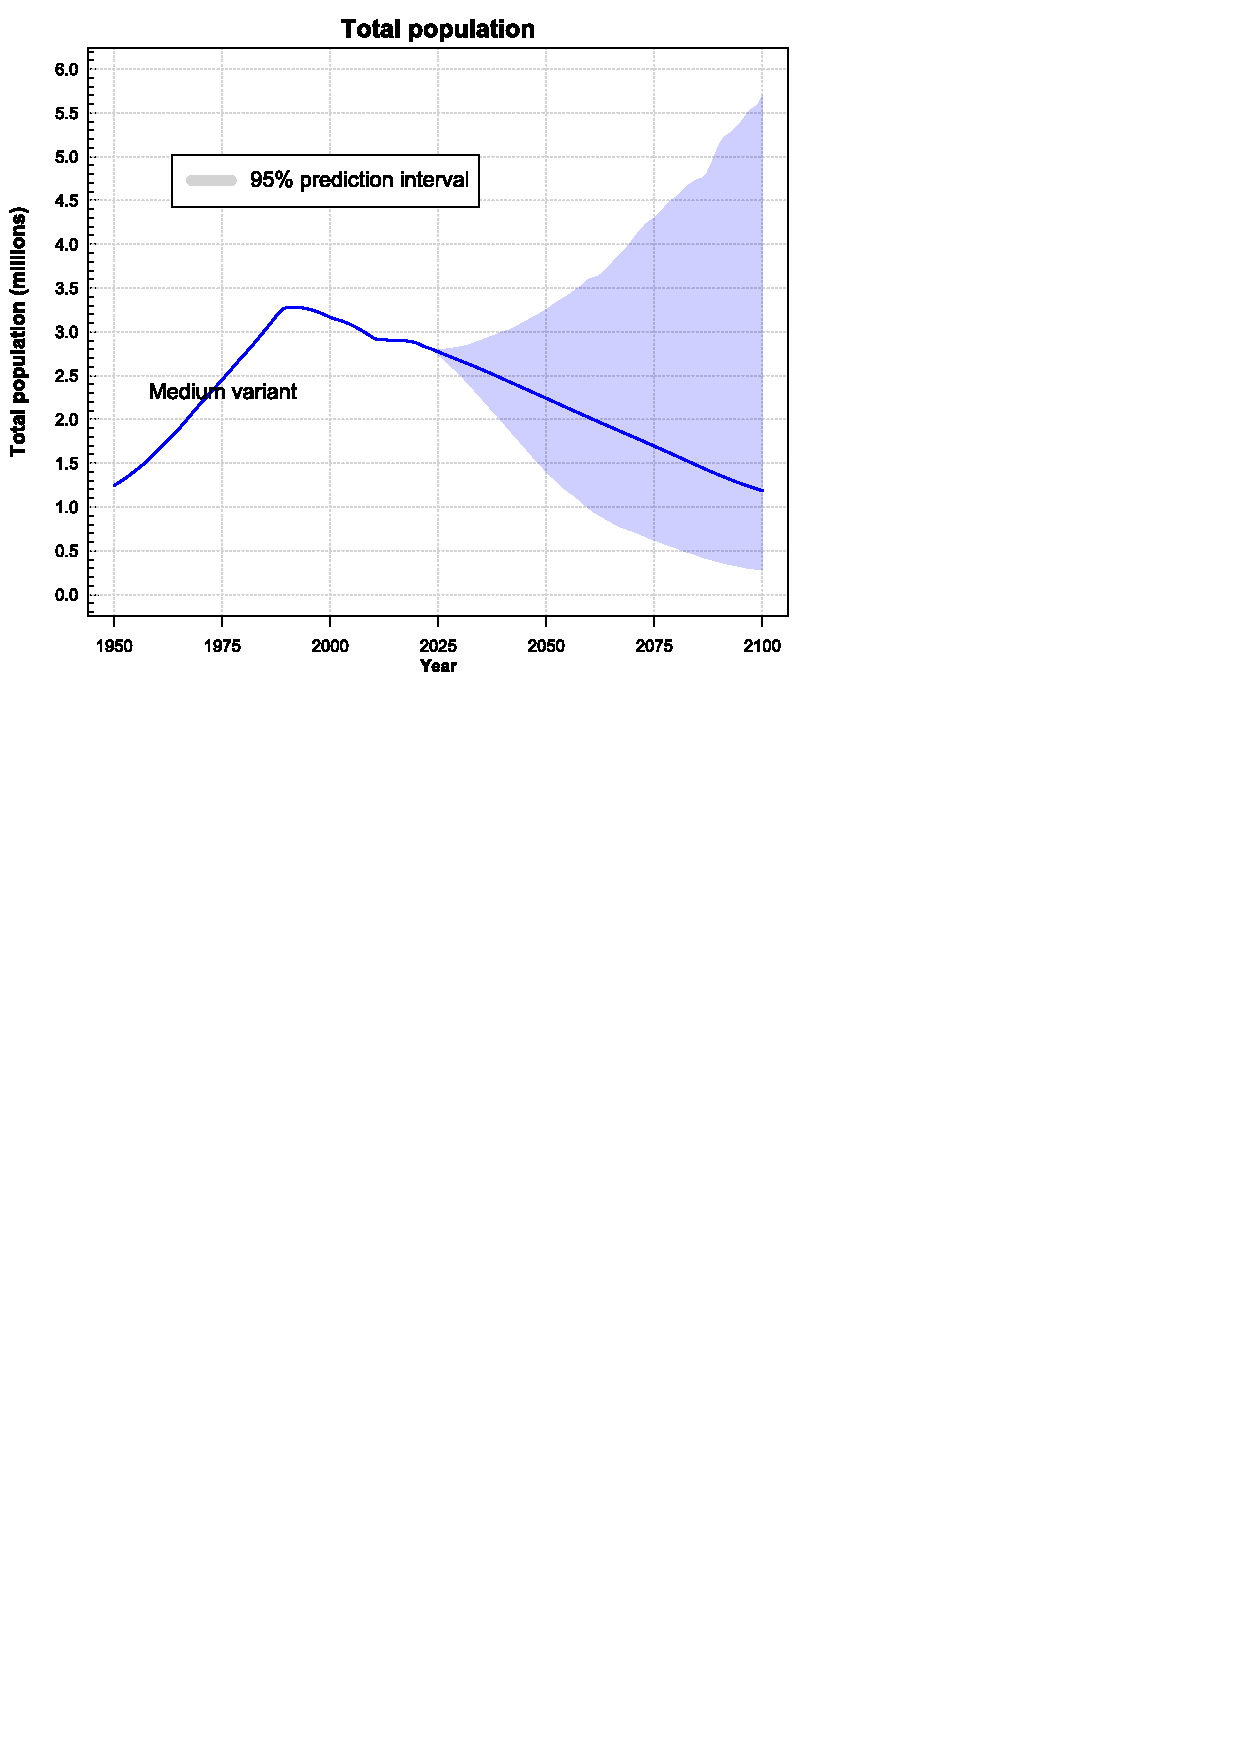
\includegraphics[width=\textwidth]{photos/1-Total population.html.pdf}
    \end{subfigure}
    \hfill
    \begin{subfigure}[b]{0.32\textwidth}
        \centering
        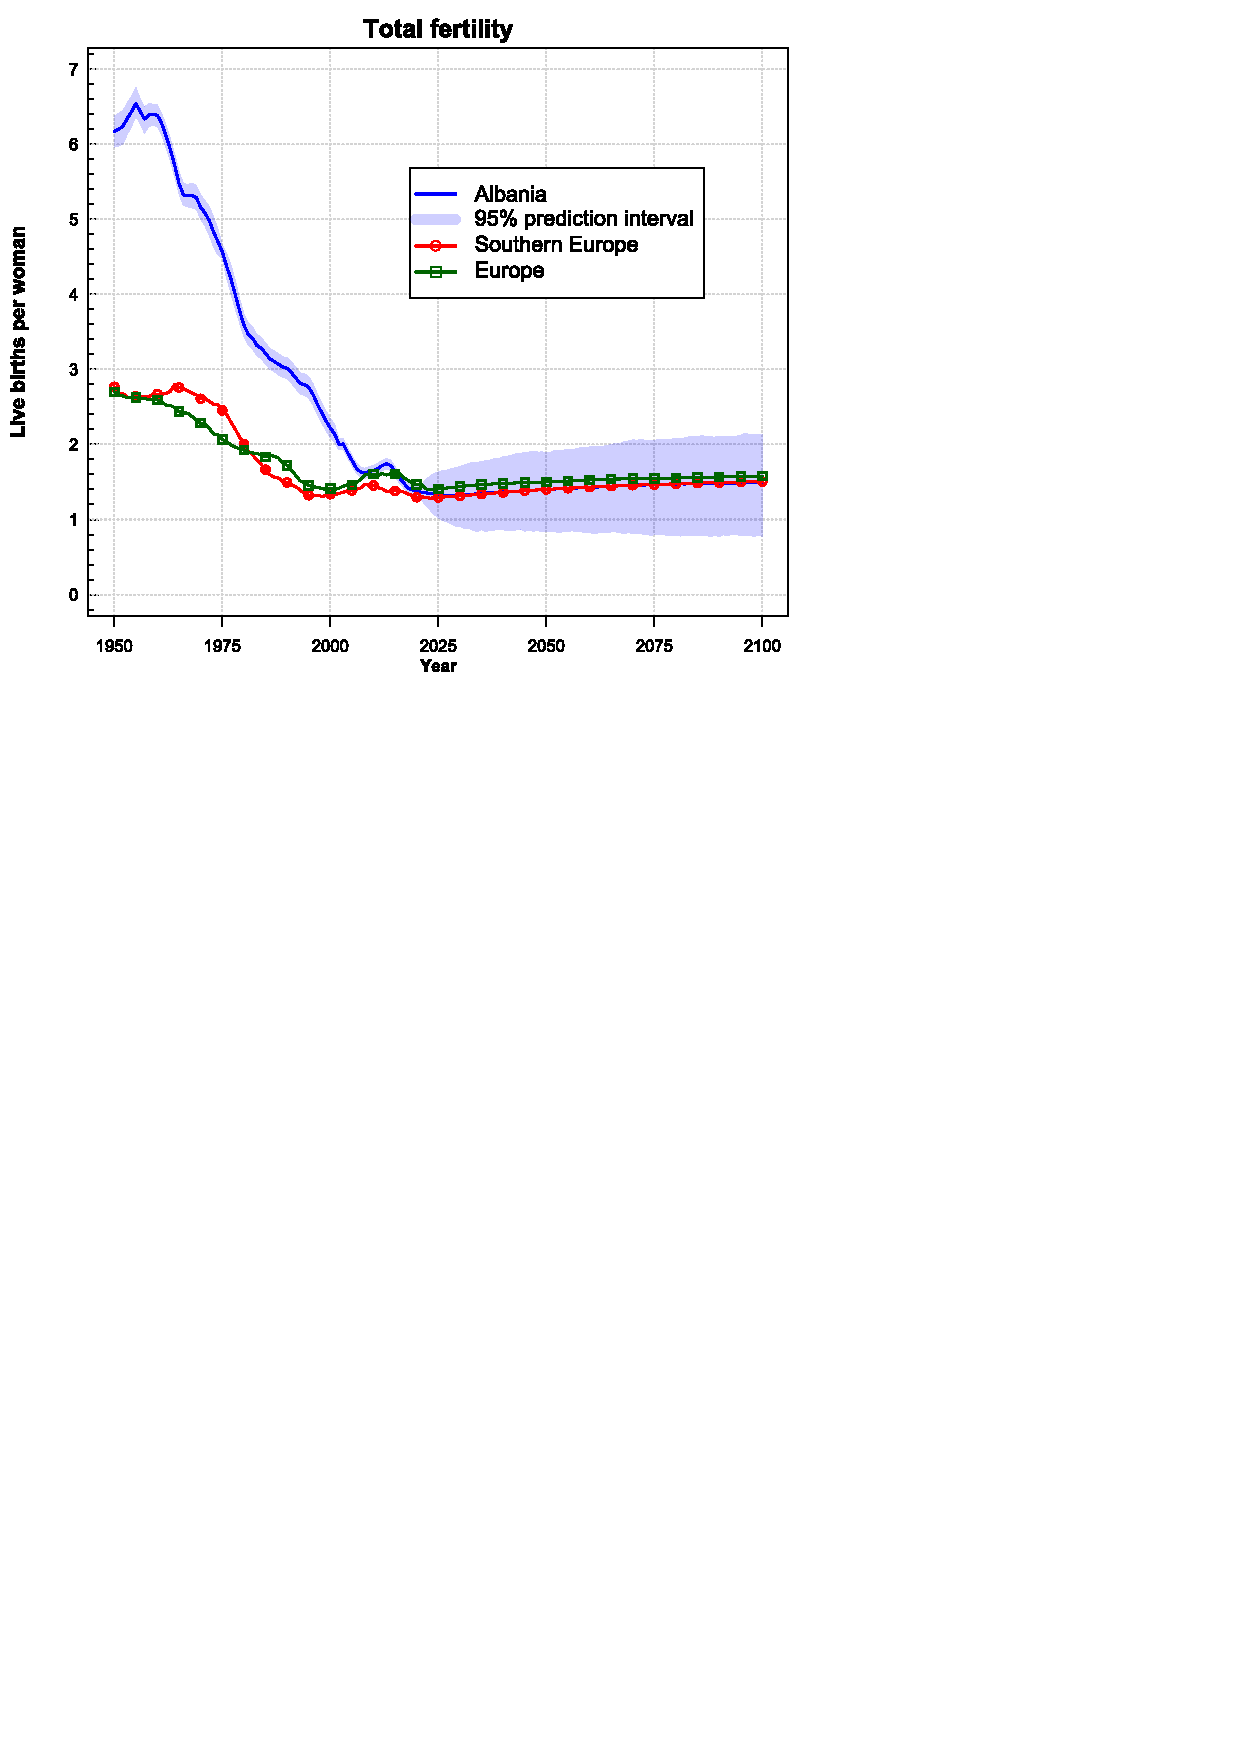
\includegraphics[width=\textwidth]{photos/6-Total fertility.html.pdf}
    \end{subfigure}
    \hfill
    \begin{subfigure}[b]{0.32\textwidth}
        \centering
        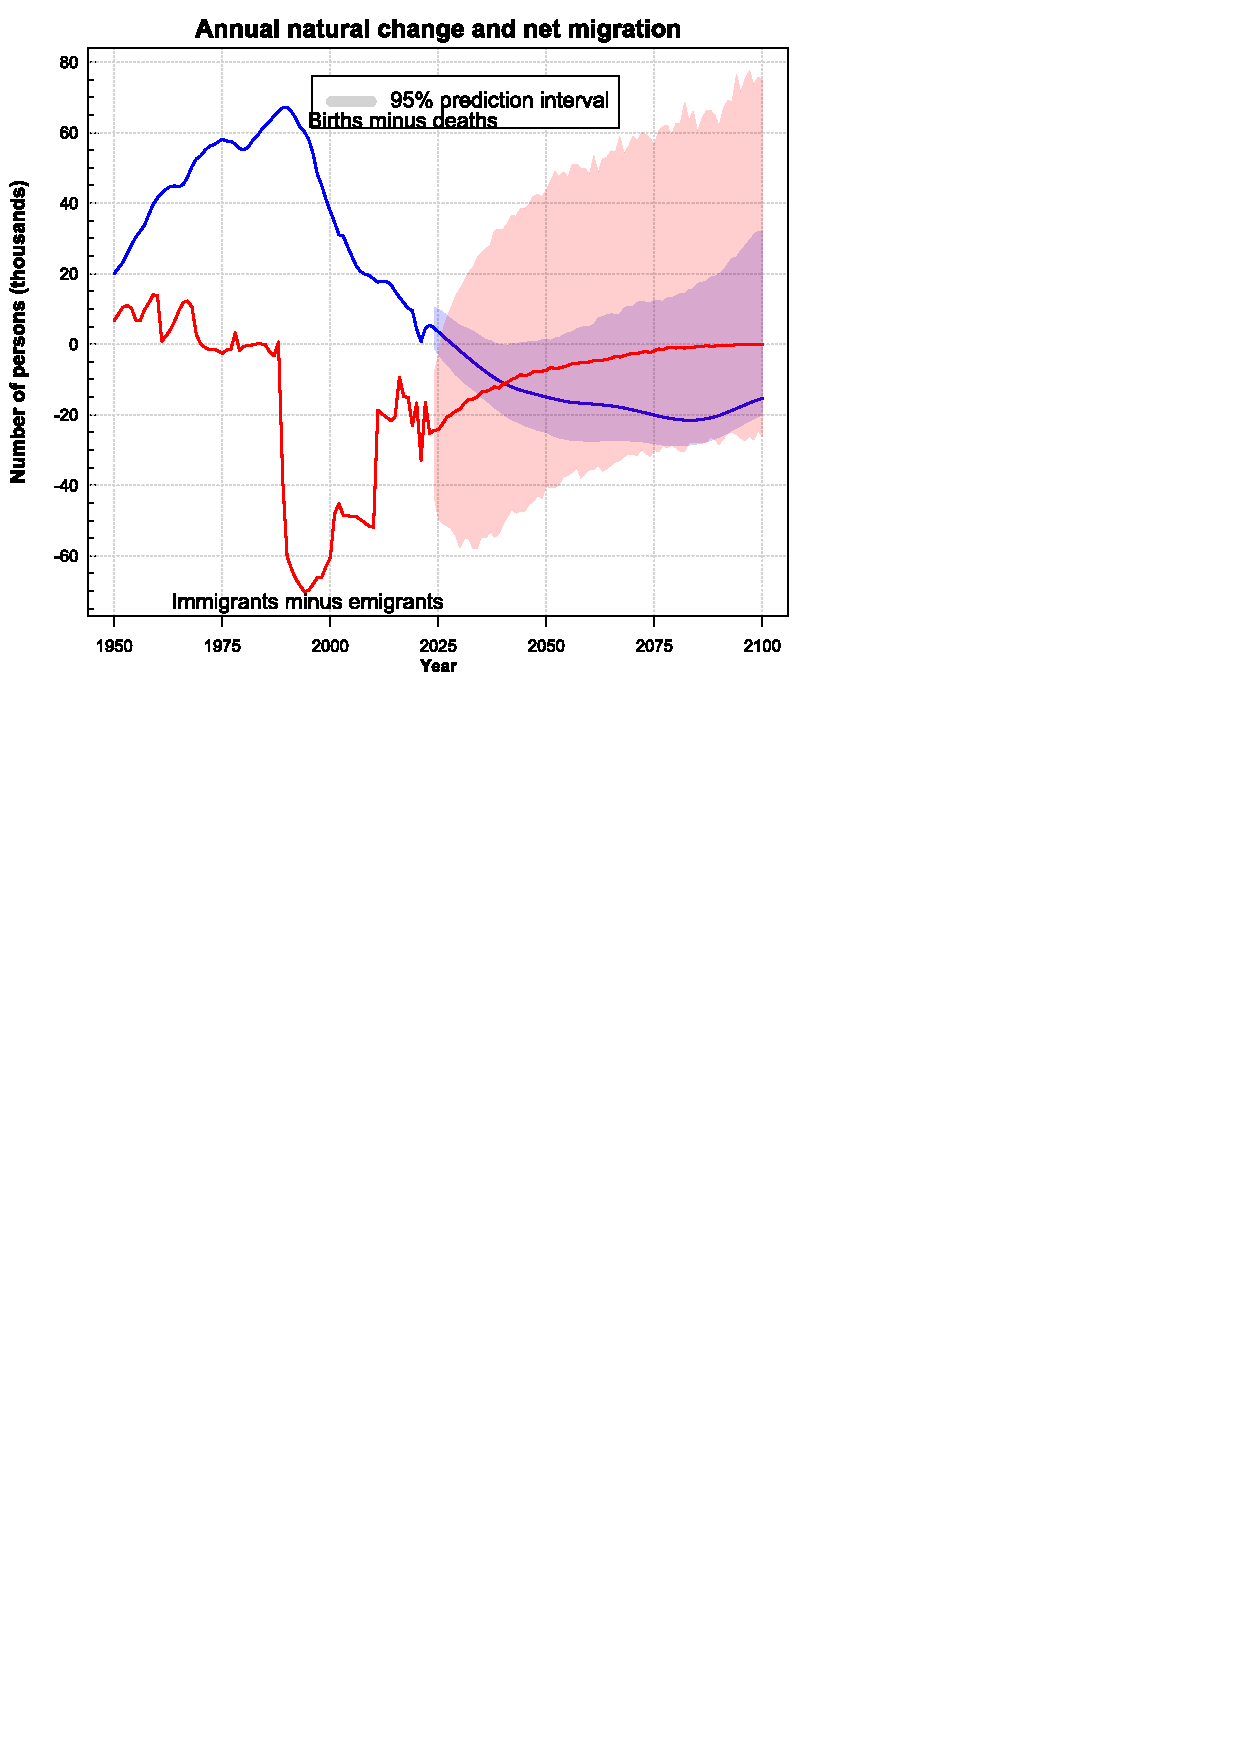
\includegraphics[width=\textwidth]{photos/10-Annual natural change and net migration.html.pdf}
    \end{subfigure}
    \caption{Graphs showing some demographic development of Albania \citep{unitednationsWorldPopulationProspects2024}}
    \label{fig:back-albaniaDemo}
\end{figure}
If it is to be granted entry into the \acrfull{eu} block, an ambition supported by its EU membership application in 2009 \citep{europeancouncilAlbaniaConsilium2025}, Albania will have to meet the demands of the EU Commission. The country will need to secure the production of renewable energy resources, such as solar power. The country also needs to increase development in rural areas, lacking institution building in these areas\citep{eucommissionAlbania2024Report2024}. Having only achieved full grid coverage for the first time in 2010 \citep{internationalrenewableenergyagencyTrackingSDG7Energy2023}, the rural population has been lagging behind the development in urban areas. Although  almost all energy production in Albania comes from hydroelectric plants, Albania tends to experience a power deficit. On average, between 2000 and 2022, they imported 20 percent of their electricity supply \citep{internationalenergyagencyAlbaniaCountriesRegions2025}. Albanian shares a power market with Kosovo, importing electricity from them through the Albanian Power Exchange\citep{albanianpowerexchangeHistoryALPEX2025}. Kosovo has 91\% of it's electricity generation from coal plants, making the imported energy from mostly fossil fuels\citep{internationalenergyagencyKosovoCountriesRegions2025}. 


\section{`Use the Sun' project background}
In 2024, Bright Products and Norsk Nødhjelp cooperated with The Door Albania to initiate the "Use the Sun" project. This project had the objectives Environmental Impact, Economic Benefits and Community Awareness - distributing \acrfull{shs} to various consumers, including private families, small companies and organizations, seeking to increase the production of clean energy and to educate communities about the benefit of solar power. More than 140 systems were delivered to participants. Most recipients were located in the northern part of Albania, near Shköder. Although different Bright models were distributed, all the systems belong to the same series from Bright Products and fall within the 30Wh to 80Wh range.

Norsk Nødhjelp has been present in Albania with humanitarian aid since 1996. Their work includes running a free daycare, delivering clothes, food and other equipment to people in need. Organizing social activities for children, youth and disabled people \citep{norsknodhjelpAlbania2025}. 

The motivation to do an evaluation of this project stems from the low amount of literature in the specific field. The research and literature on the subject of SHS are often contained to areas with no access to electricity, rather than where there is grid connection. For example This report from Rwanda \citep{asifGrameenShaktiExemplary2012} showing an exemplary case of the result of SHS in a rural off-grid area. Or this master thesis with a case study in Kenya \citep{gulbrandsenAssessingWhetherConnection2021}, making a detailed analysis about how SHS or microgrids can be implemented to increase access to electricity in a specific village.  


\section{Solar energy as a power source}
\label{ch:back:sec:solar}
\subsection{Lower costs of PV technology}
From 2010 to 2023, utility-scale \acrfull{pv} systems \acrfull{lcoe} fell from 0.460 USD per kWh, to 0.044 USD per kWh. Making PV technology's global weighted average LCOE 56\% lower than fossil fuel options 
 \citep{irena_renewable_2024}. PV system technology is expected to lower in LCOE even further. In figure \ref{fig:back-lcoe-nrl} NRL is expecting the price of residential PV to decrease substantially by 2050 \citep{nrlResidentialPV2024}. The costs decrease of PV systems help further the ambition of a green and fossil free energy mix. \citep{calvinIPCC2023Climate2023} refers to the decreased costs of solar allowing some regions to reduce their overall energy costs by replacing unsustainable energy sources with solar power. Also emphasizing that there needs to be a transition to renewable energy sources to reduce the emissions of greenhouse gasses. With the eminent future going towards an increase of \SI{1.5}{\celsius} above average within 2040, emissions needs to be reduced quickly \citep{calvinIPCC2023Climate2023}. 

\begin{figure}[H]
    \centering
    \begin{subfigure}[b]{0.48\textwidth}
        \centering
        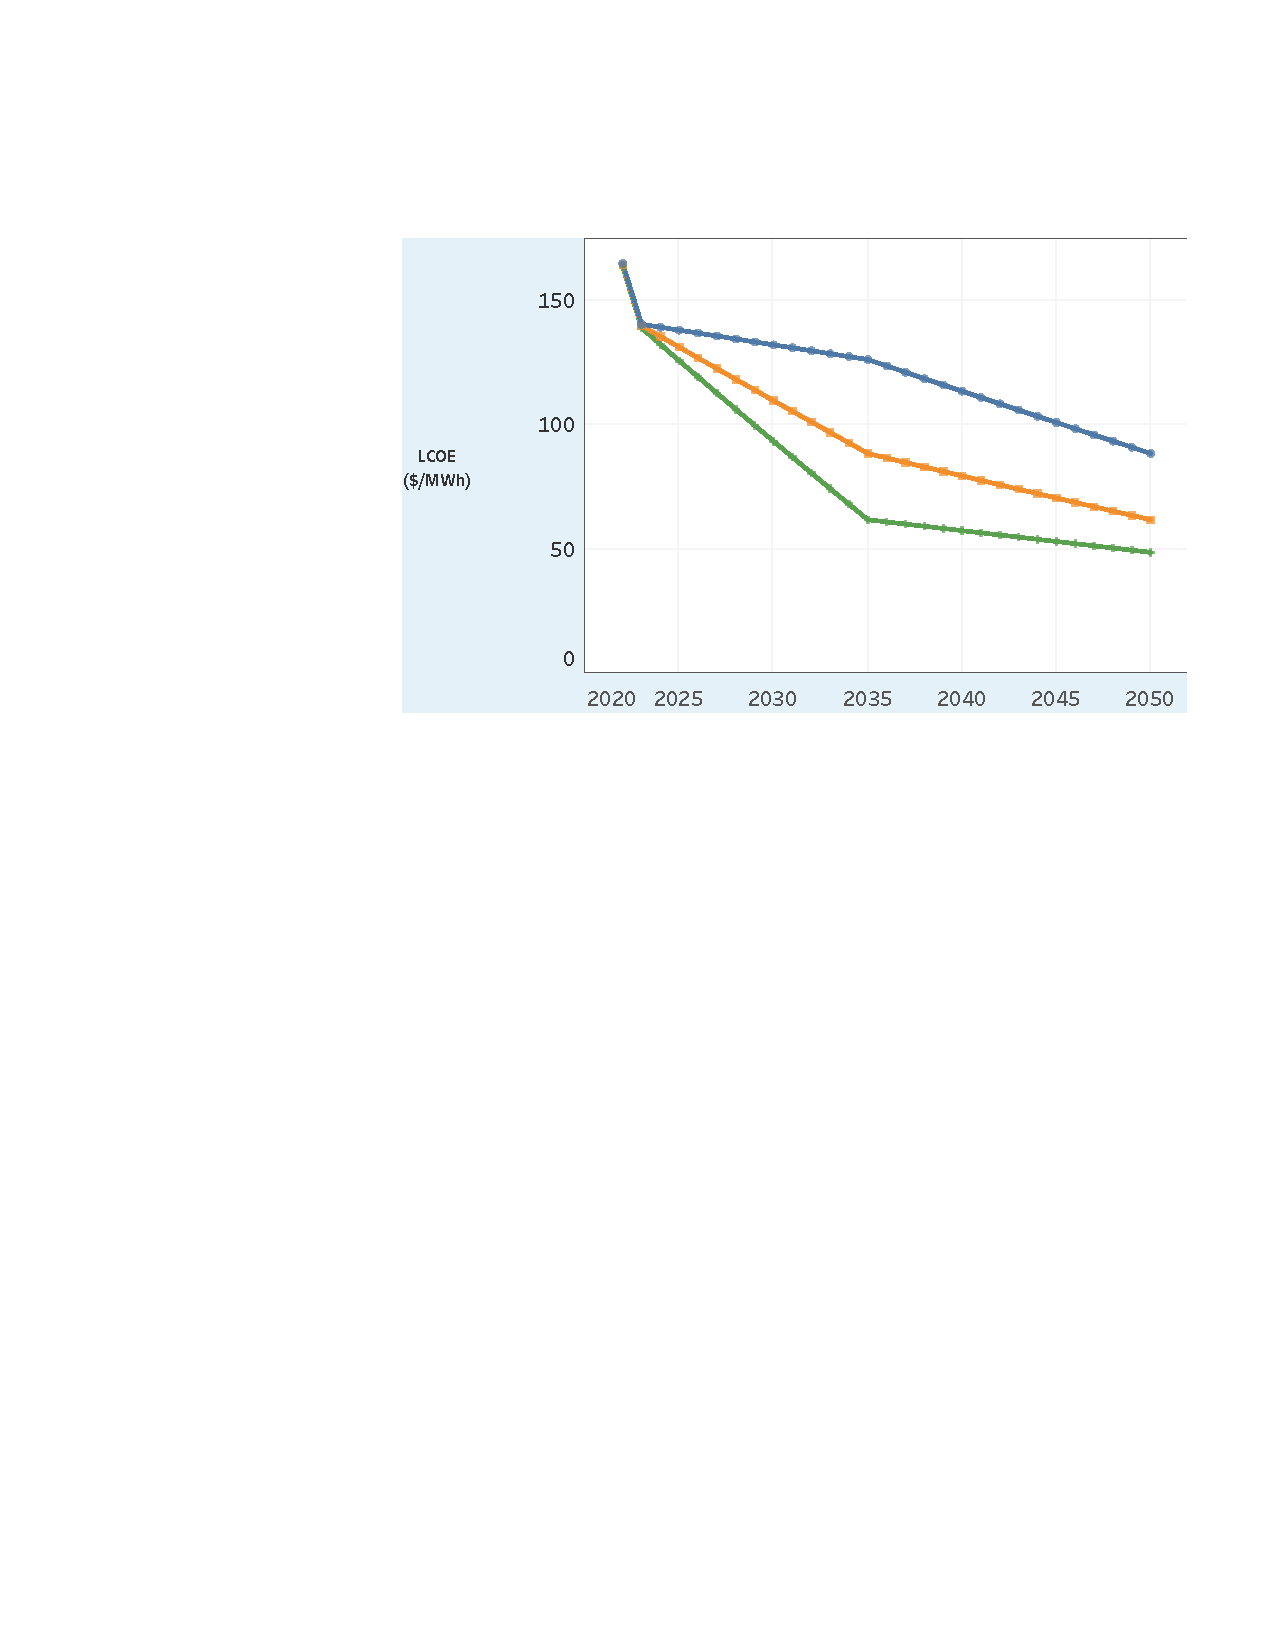
\includegraphics[width=\textwidth]{photos/LCOE_ResidentialPV_NRL.pdf}
        \caption{NRL prediction for residential PV systems. Using scenario of average 4,5 to \SI{5}{\kilo\watt\hour\per\square\meter\per\day}. The three scenarios are conservative (blue), moderate (orange) and advanced (green).}
    \end{subfigure}
    \hfill
    \begin{subfigure}[b]{0.48\textwidth}
        \centering
        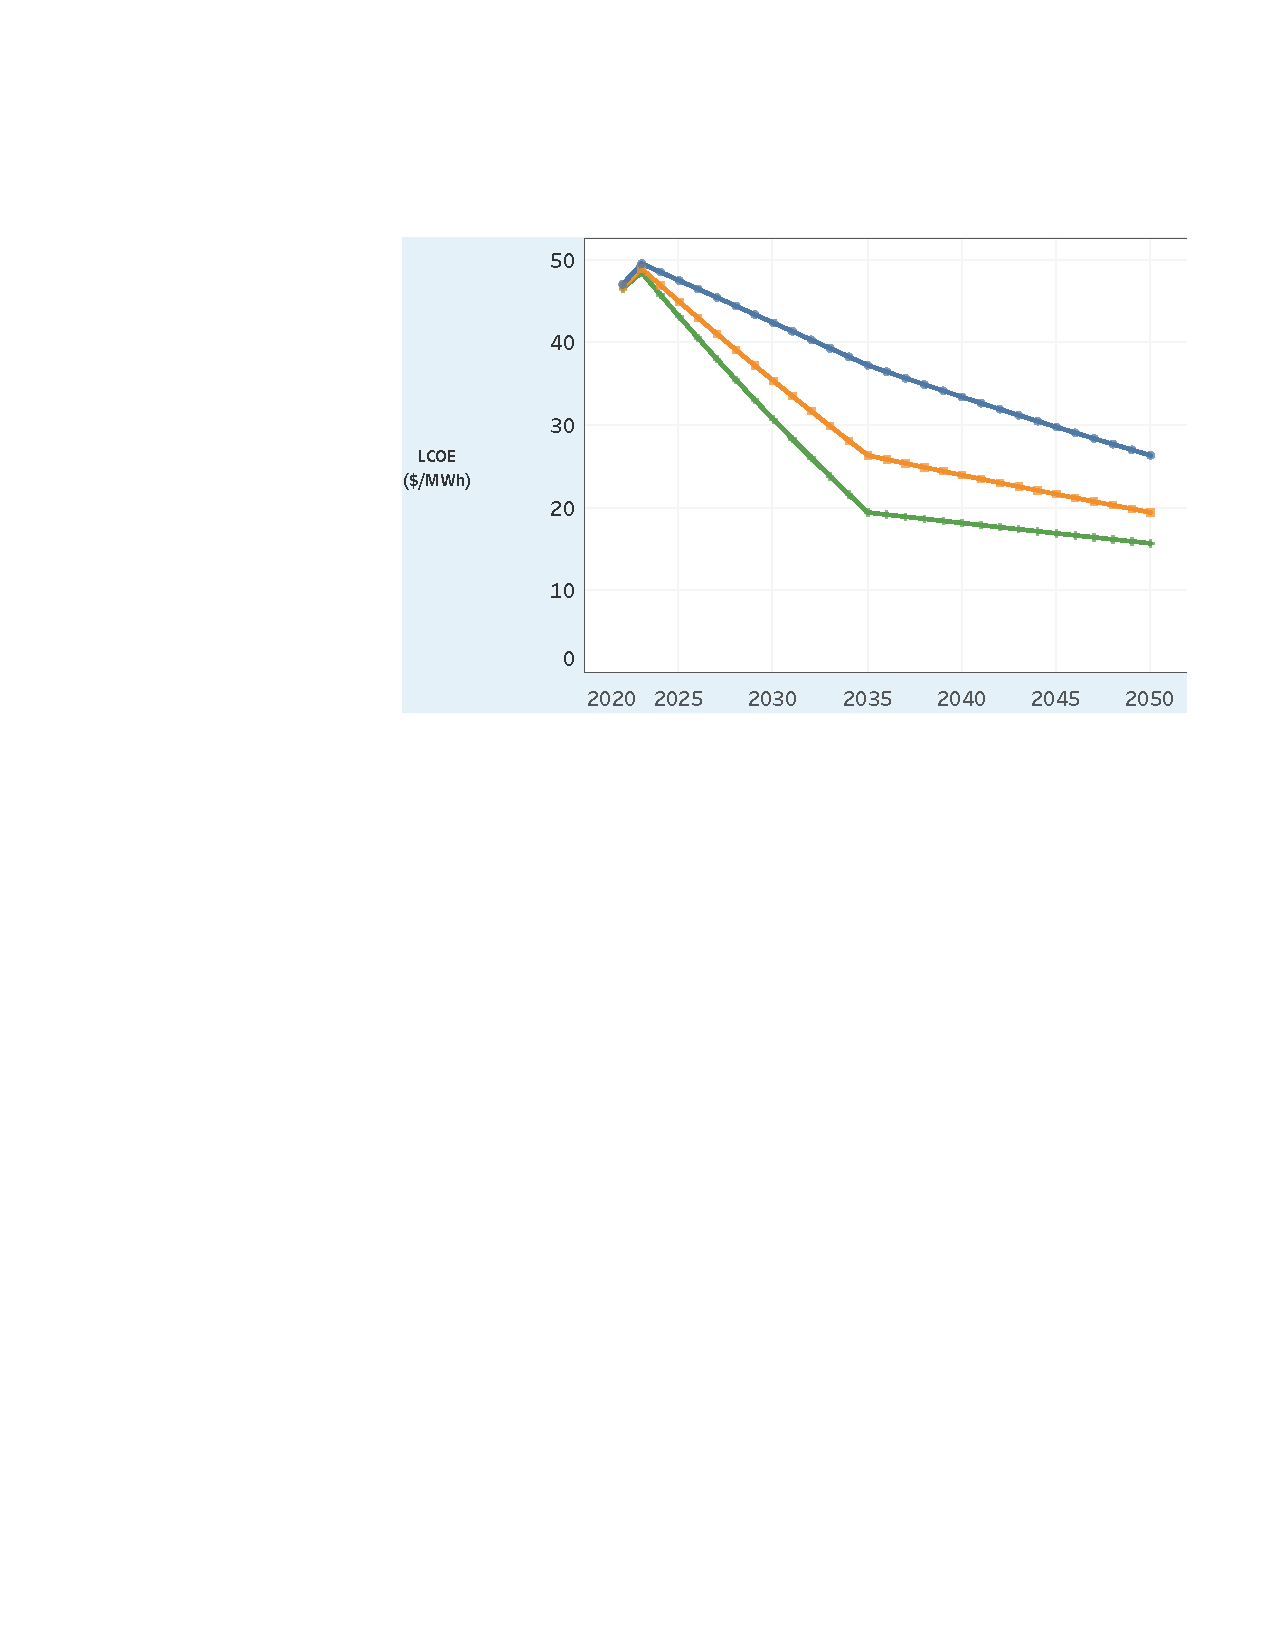
\includegraphics[width=\textwidth]{photos/LCOE_UtilityPV_NRL.pdf}
        \caption{NRL prediction for utility PV systems. Using scenario of average 4,5 to \SI{5}{\kilo\watt\hour\per\square\meter\per\day}. The three scenarios are conservative (blue), moderate (orange) and advanced (green).}
    \end{subfigure}
    \caption{}
    \label{fig:back-lcoe-nrl}
\end{figure}

\subsection{Solar energy in Albania}
Solar energy accounted for 2.3\% of electricity production in Albania in 2022\citep{internationalenergyagencyAlbaniaCountriesRegions2025}. Green Energy News Balkan posted an article claiming it is now 6\%, and that there is plans to further increase the capacity by  235MW \citep{igortodorovicSolarPowerDevelopers2025}. In January 2025, Albania, Italy and United Arab Emirates signed a three-way energy cooperation deal. It's purpose was to increase Albanian's solar and wind production, and to export power to Italy via underwater cables\citep{euronewsgreenItalyAlbaniaAgree2025}. These news show that Albania seeks to expand their capacity within solar energy. 

A 2021 report by International Renewable Energy Agency states that Albania's technical potential for the deployment of solar PV is estimated at 2378 MWh. Also purposing a plan for 2030 of an installed capacity of 1697 MWh\citep{irena_renewables_2021}. The report also talks about the importance of raising public awareness to the adoption of the technology. Figure \ref{fig:back-albaniacapacitymap} shows the areas that the report suggested for installing PV systems. The areas suggested mostly occur close to the coast, where the land is flat. Skhöder, the area most relevant for the project, is marked as a suggested spot. 

\begin{figure}[H]
    \centering
    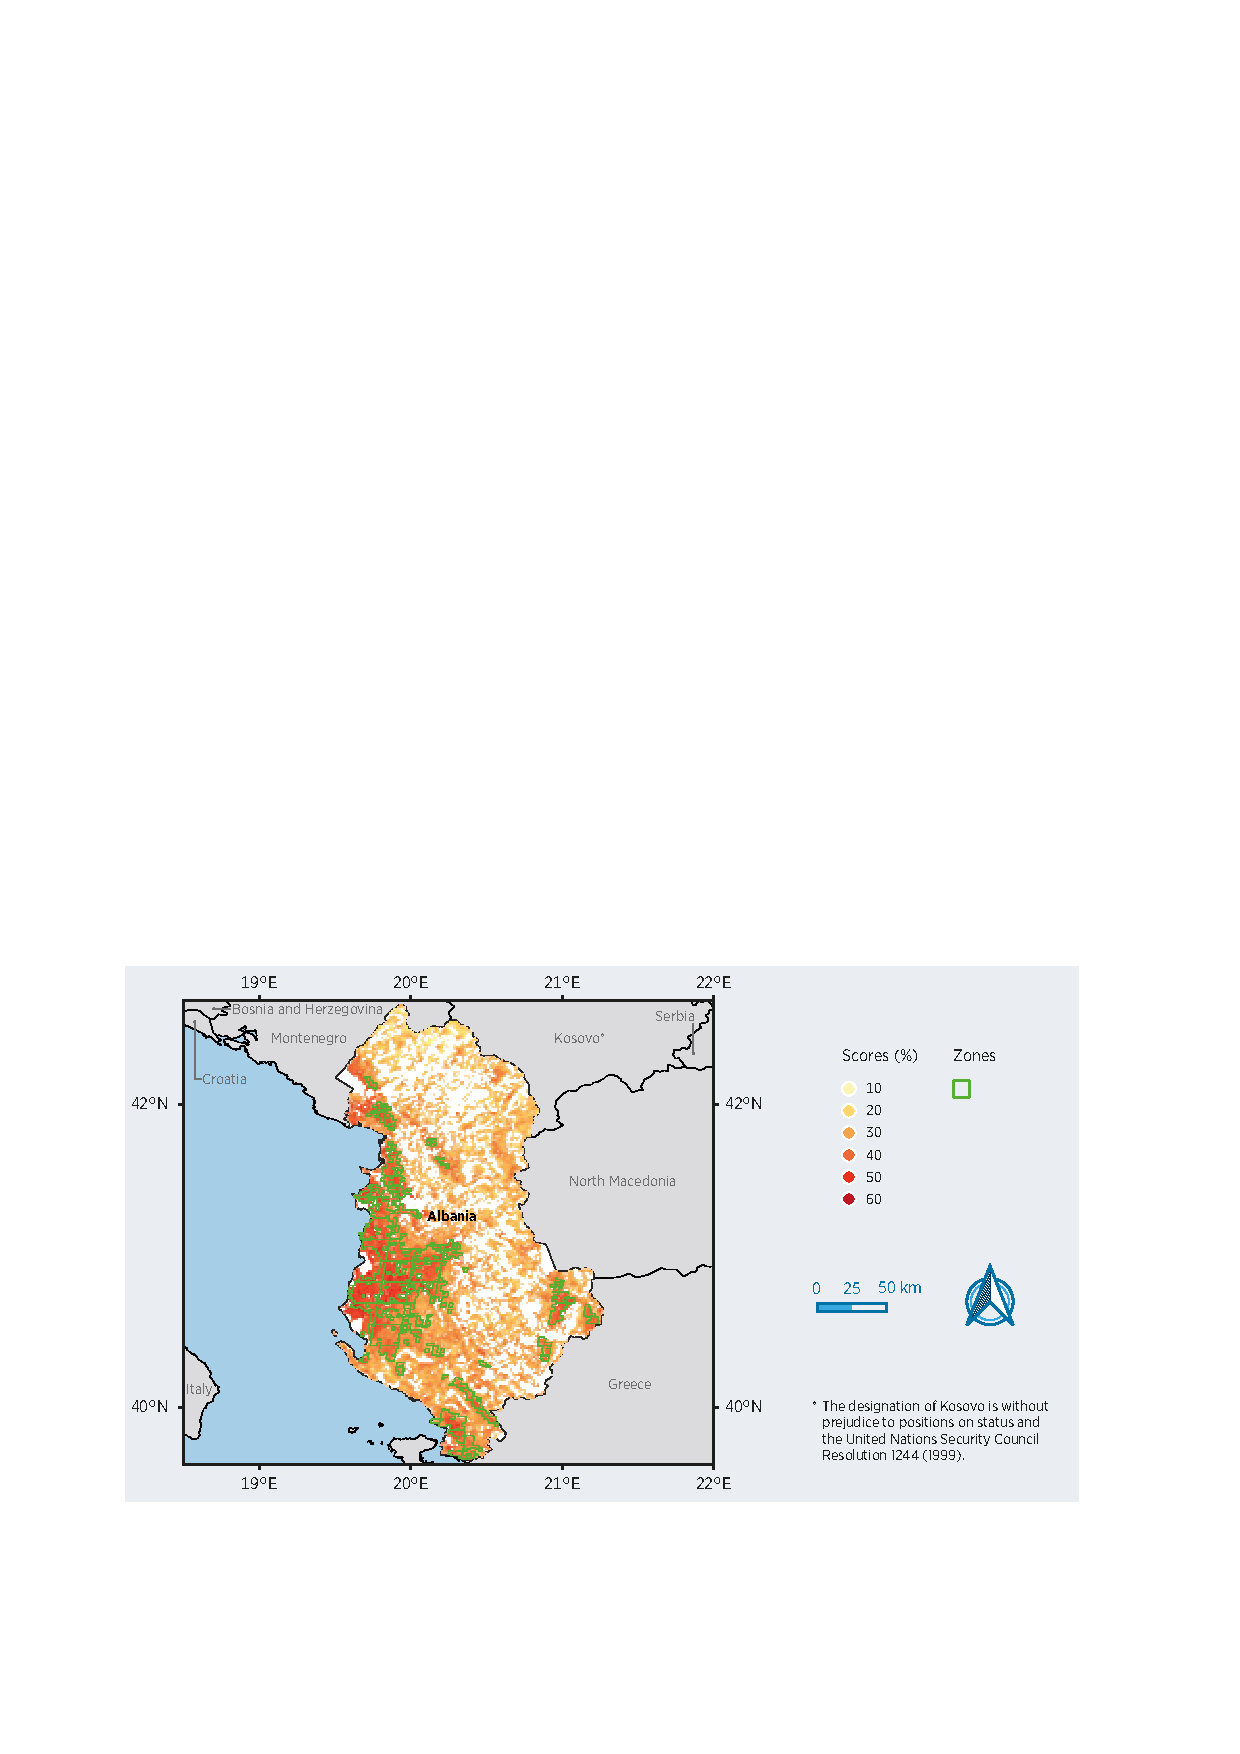
\includegraphics[width=\linewidth]{photos/Albania_solarPVCapacity_map.pdf}
    \caption{Suitable areas for solar PV development and zones with highest potential \citep{irena_renewables_2021}.}
    \label{fig:back-albaniacapacitymap}
\end{figure}

\subsection{SHS as a power source}
\acrfull{shs} have been used for decades to provide renewable solar energy to areas without access to electricity. Consisting of a simple design with a solar panel, battery and lighting - SHS is a robust and easy product to use. Making use of solar power these products are often introduced in areas with high irradiance, such as Sub-Saharan Africa. Introducing SHS to developing countries has been shown to introduce problems. Access to skilled technicians and general knowledge about the product has been highlighted as a reoccurring problem \citep{chaureyAssessmentEvaluationPV2010}. The high initial cost of purchasing a SHS is another one of the main causes hindering adoption of the technology, sometimes reaching up to half of the user's income. Product quality, maintenance and user training have also been shown to be barriers to entry\citep{girardeauHouseholdSolarAdoption2018}. 


\section{Existing Approaches/Baselines}
Since there are a lot of different cases for SHS, there are also a lot of different approaches analyzing a SHS project. Most studies look at the \acrfull{lcoe}, and in general, look at either the technical design of the systems or economical viability of the systems. These fiscal measures serve as a solid baseline for a project's success, but often do not tell the entire story. \citep{thomasPESTLEAnalysisSolar2021a} did a \acrshort{pestel} analysis for a broader evaluation of the subject. Though the format offers a wider result, they found a lack data in their legal and environmental section of the analysis. This is caused by the limited amount of available research and information to evaluate this. 

One study proposes a new way of analyzing the success of SHS projects\citep{holtorfModelEvaluateSuccess2015}. It evaluates based on self set goals for each project and the different stakeholders in the project. Each self set goal is then ranked by  importance and degree of achievement, giving it a score based on the stakeholders subjective experience. 

\citep{lervikTechnoEconomicAnalysisRural2021} use simulation and load profiles to create an estimated value for the panels and their effect. This approach offers a solid foundation for the production capabilities of the equipment. 

SHS typically does not store data about product usage such as battery charge cycles and electricity usage. Recording and storing data would increase cost, and demand some power to maintain the circuit. \citep{lopez-vargasIoTApplicationRealTime2019} have created a logging feature that communicates with 3G to send data as consumption, production, battery state and weather data. Although their solution is low cost compared to commercial alternatives, the conclusion is that this is costly on small-scale systems.

To account for a lack of data tracking from the equipment, \citep{mannesEnduserEvaluationSolar2017} used a load profile based on detailed interview questions.  
Data are gathered on when the power was used, and how much it was used within a day. Using these data \citep{mannesEnduserEvaluationSolar2017} can also compare the daily load against the theoretical charge given in various days, to see how the production and consumption match.



One way to gather data is through qualitative research. Interviews with consumers about their experiences are used in several SHS studies e.g., \citep{mannesEnduserEvaluationSolar2017},\citep{asifGrameenShaktiExemplary2012}, \citep{beyeneSocioeconomicImpactsSolar2024}. On the one hand, semi-structured interviews provide a good baseline, offering the possibility to ask additional questions outside of the structured questions. On the other hand, structured questions give the possibility to easily compare results and organize the data.

Sub-Saharan Africa is often used as study area in the literature. \citep{kizilcecSolarHomeSystems2020} shows that the most common topics for SHS in Sub-Saharan Africa are the business aspects and the design of the systems. More research around the institutional barriers, and the regulatory framework is called for \citep{kizilcecSolarHomeSystems2020}.







%!TEX root = ../thesis.tex

\chapter{Data}
\label{ch:data}
%\section{Approach}
%Since there has not been done many research projects about \acrshort{shs} in Albania, this thesis will use a similar approach to other studies. The most common from Sub-Saharan Africa being the socioeconomic aspect, we will apply this evaluation. We will look at the usage of these systems and compare that to their capability. Their energy savings will be compared towards their cost. 
\section{Qualitative research}
We use a qualitative method for the analysis of consumption and general usage of the systems. To acquire this information we had a field trip with interviews of the projects participants. The field trip consisted of two days to gather our field data. Since we anticipated fewer than 30 interviews, the of data should be mostly qualitative. This journal article about qualitative interviews \citep{malterudSampleSizeQualitative2016} explains how we can increase our "information power" when narrowing down the research area. Giving more credibility to the data when it has less possibility for errors. Meaning we should try to find as many participants in the same situation as possible. The systems where donated to various organizations and households, but we focused on poor families living in rural areas.

Narrowing down to mostly poor rural households gave us data that would be more similar than data from randomly chosen participants. Poor families often live with some of the same issues and problem. They often have a restricted household economy, and tend to be aware of every cost they have. As poor families living in rural areas were also the largest group, they were the natural choice for the study. Two interviews were done with organizations that had several systems, were one was a social house for disabled elderly people - and the other was an eco-social farm. Among these, only the consumption data of the social house was deemed relevant for the study. As both would be anomalies in household compositions and economics. The social house consumption data was deemed relevant as it had the same purpose for usage as households.


\section{Simulation and Load Profile}
The \acrshort{shs} don't record any production in the system, meaning there is no way to extract the data from the system. Knowing the size of the PV panel and the battery size, we can use simulation to estimate this. With this production data, we can see the differences in seasons and analyze if the systems will last with it's projected use every day. 
To analyze the electricity usage of the systems, we create a load profile. This gives some quantifiable data to help analyze the usage of the system. Asking the specific consumption questions in Appendix \ref{apx:ftquestions}, we can create a profile of daily usage to estimate the consumption. Combined this will give us how much the systems are utilized based on their capability and actual usage. Simulink was used for all simulations that were not gathered from \acrshort{pvgis}.
%\subsection{Metrics}
%To analyze the socioeconomic value of the systems, we use metrics that are common in economical analysis. LCOE is common in energy economics and gives us a good base to work from. These systems are generally not known for being cheap for users to buy, and therefore they need to have a sufficient energy yield. To see if any household should invest in this we will use payback time. SHS is not a common product outside of off-grid areas, and is therefore not easily compared with payback time. As this area is grid connected, the payback can directly be compared to the cost of consumption from the grid. How utilized the system is, will be needed for all of these metrics. The utilization rate is also relevant to look at as it's own metric. If the utilization rate is low, these systems may have been better aid somewhere else. 

%To analyze the social benefits, we compare answers and discuss the effects. The daily load profile together with the simulated production will be used as the baseline for most of the economical evaluation.

%\subsection{Discussion}
%For the less tangible evidence from the interviews, we will discuss this in the results. Here we will look at what factors that are important to consider besides the metrics. 


\section{Field trip}
During the start of April 2025, the field trip took place in Shköder, Albania. During the field trip, "The Door Albania" organized the interviews with the participants of the project. The interviews were translated by representatives from "The Door Albania" between Albanian and English. Some data is gathered from observations, although most of it is from recorded interviews. All participants signed a written agreement to let us use their data in this study, and all data was anonymized to preserve their data privacy right. The study was also approved by Sikt, the Norwegian Agency for Shared Services in Education and Research.

\subsection{Observations}
Which type of SHS they had was observed and noted down for each interview. The angle and azimuth was also estimated with pictures and notes from the household visits. Observations of where the lights were placed, and how many lights were mounted was also noted with pictures. General observations for use in the discussion includes the state of the household, and their attitude towards the system. 

\subsection{Interviews}
There were conducted 14 interviews encompassing 20 SHS in total. Most of the interviews where one-to-one, each of them owning one system. Some participants had multiple systems, and some interviews where done with multiple participants. Households consisted of 14 of the total systems on 11 interviews, where one interview was done with three households together. Off-gird sheds was two interviews with two total systems. One social house interview being the remaining four systems. Poor households tended to answer a lot of the same answers, resulting in neatly gathered data.

%!TEX root = ../thesis.tex

\chapter{Method}
\label{ch:method}


\section{Energy simulations}
\subsection{Production}
Since this project cannot gather data of production from the systems, a simulation is useful for creating an estimation of this. In this case, we have specifications of equipment and location to test out. The systems are delivered from Bright, and are three different sizes. The three systems are given in table \ref{table:product_specifications}. 

\begin{table}[h]
\centering
\begin{tabularx}{\textwidth}{|X|X|X|X|}
\hline
\textbf{Product name} & \textbf{Battery capacity [Wh]} & \textbf{Panel size [Wp]} & \textbf{Total lumen} \\ \hline
BH 300                &            29                    &          10                 &         360               \\ \hline
BH 600                &              58                  &          20                 &           760             \\ \hline
BH 800                &              80                  &         40                  &            1400            \\ \hline
\end{tabularx}
\caption{Product specifications of Bright SHS}
\label{table:product_specifications}
\end{table}

Using this we have three different scenarios we can simulate with. Further we need to locate the weather data to use for this. The \acrfull{pvgis} can be used as a trusted data source to simulate with specific weather data for a location\citep{huldNewSolarRadiation2012}.

Using that we have a 40Wpp PV panel, we can use the PVGIS to simulate the power generation for each month. The PVGIS assumes a 14\% power loss in the transmission. Since we don't have any more accurate data, this will be used in the simulation. Potential soiling will be added as power loss in results. On figure \ref{method:fig:wattage_generation_PV40wpp} we can see how each month differs in the power generated. Each month has been given a mean to account for good or bad days. This will give us a good indication of what a typical day will generate during a day, and when it will generate the power. When we combine this with a daily load profile, we can analyze well the system is utilized. 

\begin{figure}[H]
    \centering
    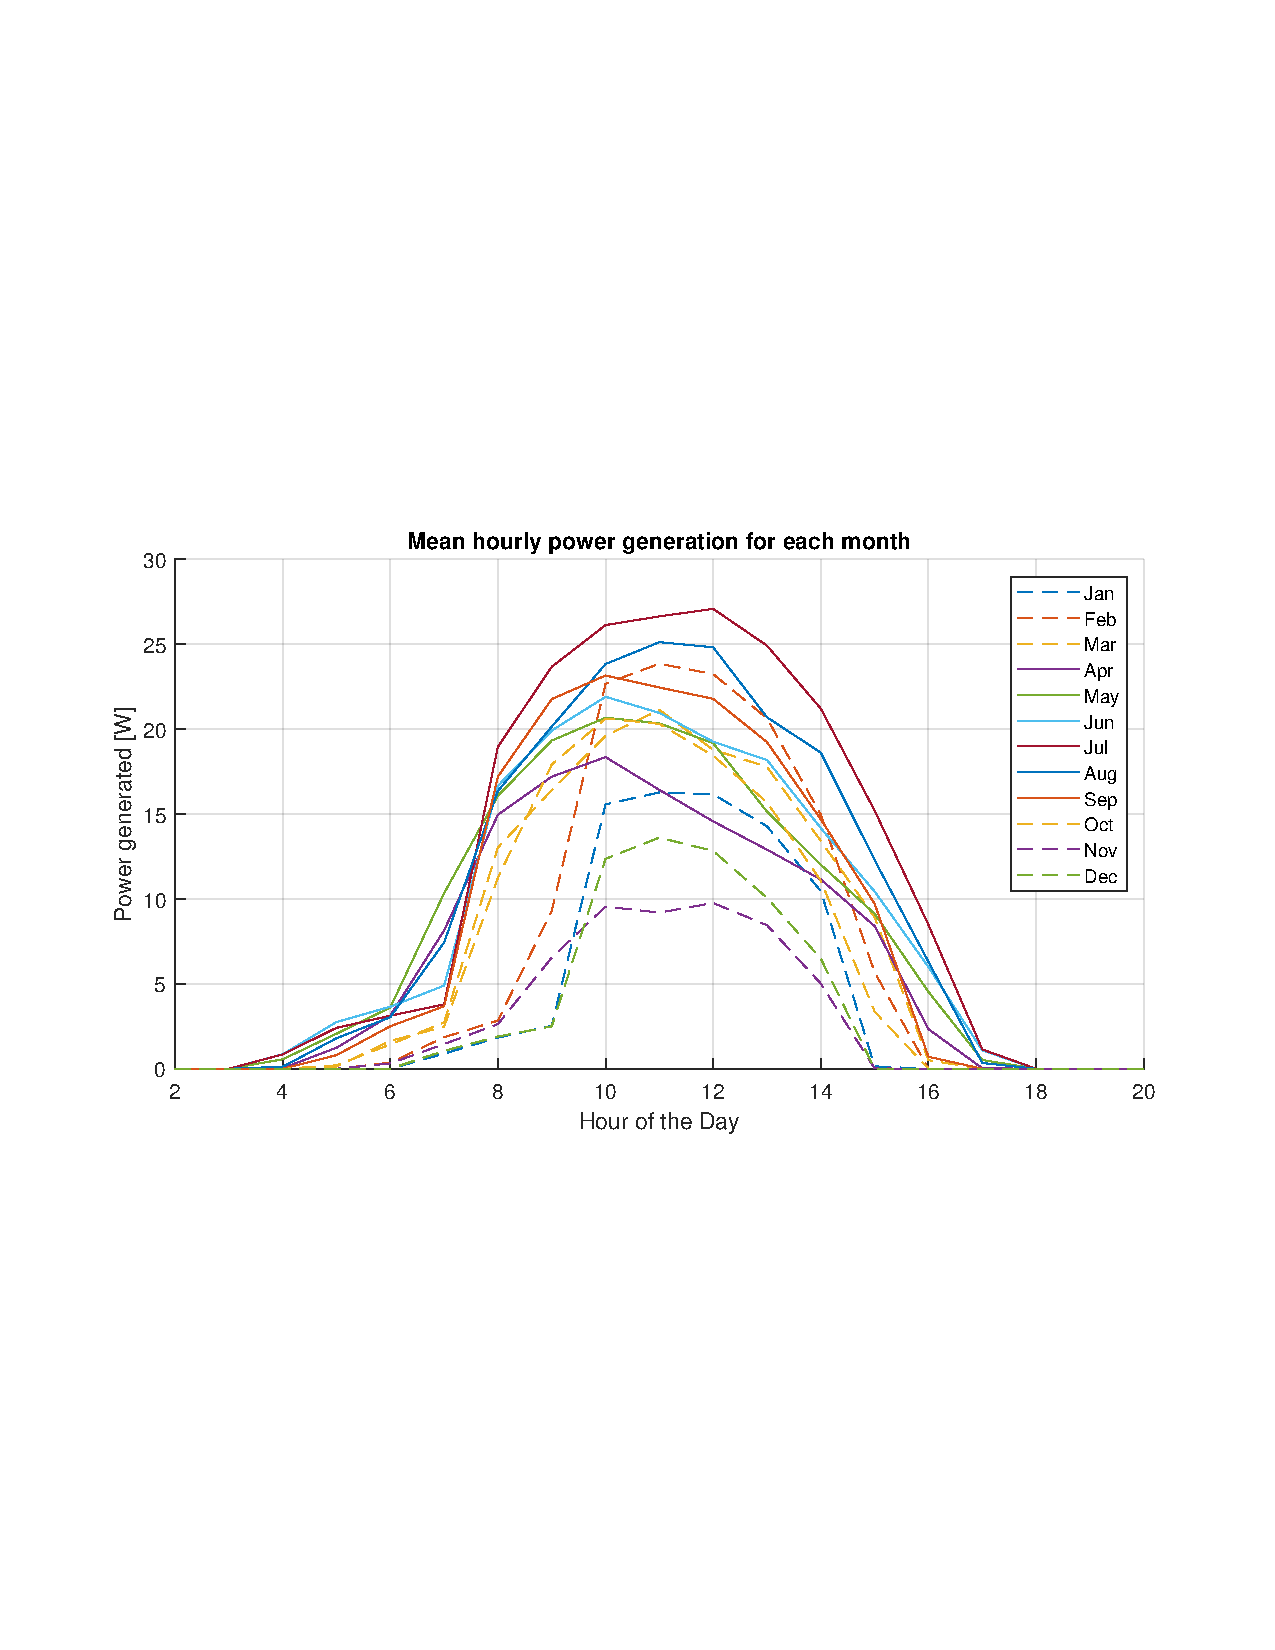
\includegraphics[width=\linewidth]{photos/Watt_generated_Shkoder.pdf}
    \caption{Power generation from a 40Wpp panel in the Shkodër region with tilt angle $\alpha=35\degree$, and azimuth $\phi=23\degree$.}
    \label{method:fig:wattage_generation_PV40wpp}
\end{figure}

The months with the least daylight has been given a dotted line, and the ones with the most have a solid line. From this we can see that the trend of most light in "winter" months is not always true. February and April will be almost equal in this simulation, showing how much factors such as rain, clouds and angle will affect the panel power generation. 

In table \ref{method:table:wattage_generation_per_month_all_panels} we can see how much each is generated for a typical day, here the values confirm what the graph is showing.
\begin{table}[H]
\centering
% For bedre talljustering i X-kolonner kan du vurdere >{\raggedleft\arraybackslash}X,
% eller for optimal talljustering, bruk siunitx-pakken og S-kolonner.
% For enkelhetens skyld beholder vi X-kolonner som i din originale tabell.
\begin{tabularx}{\textwidth}{|X|S[table-format=3.1]|S[table-format=3.1]|S[table-format=3.1]|}
% table-format=3.1 betyr opptil 3 siffer før desimaltegnet, og 1 siffer etter.
\hline
\textbf{Month} & \textbf{40Wpp [Wh]} & \textbf{20Wpp [Wh]} & \textbf{10Wpp [Wh]} \\ \hline
January        & 78.1                & 39.1                & 19.5                \\ \hline
February       & 125.4               & 62.7                & 31.4                \\ \hline
March          & 133.9               & 67.0                & 33.5                \\ \hline
April          & 128.9               & 64.4                & 32.2                \\ \hline
May            & 153.5               & 76.7                & 38.4                \\ \hline
June           & 160.7               & 80.4                & 40.2                \\ \hline
July           & 203.6               & 101.8               & 50.9                \\ \hline
August         & 180.9               & 90.5                & 45.2                \\ \hline
September      & 157.7               & 78.9                & 39.4                \\ \hline
October        & 122.9               & 61.5                & 30.7                \\ \hline
November       & 52.9                & 26.5                & 13.2                \\ \hline
December       & 60.8                & 30.4                & 15.2                \\ \hline
\end{tabularx}
\caption{Estimated daily energy production for 40Wpp, 20Wpp, and 10Wpp panel}
\label{method:table:wattage_generation_per_month_all_panels} % Endret label for unikhet om nødvendig
\end{table}
For all three systems, November, December and January is the only months that the daily production will not exceed the battery capacity. Incomplete charges can over time lead to an empty battery. It could then take several days with minimal use for the system to get fully charged again. 

These production numbers assume optimal angle and azimuth. In results chapter \ref{ch:results}, we look at both the average azimuth and the tilt angle. We will also have to account for other loss factors, such as soiling. Then we can do a more precise estimation of the daily production of the PV panel. 


\subsection{Consumption}
To gather the daily load profile, we will have to ask questions from the participants. Based on their answers we can create a daily load using the known power of having the lights on, or USB-A power delivery. The questions used for this data gathering needs to gather both how much power is used, and when it is used. There will always be some uncertainty around the numbers, and the actual usage will vary from day to day. 

Seasonal variation of the consumption is hard to measure, but can be estimated from the answers given. The difference between the shortest and longest day in Shkodër is about six hours\citep{steffenthorsenSunriseSunsetTimes2025}, meaning the systems production and consumption will vary due to seasonal differences. Longer nights leads to more usage of light from the system. Shorter days reduces the time for the panels to charge the system. Although the production is simple to find accurate data for, the seasonal differences of consumption is harder.

The duck curve is used to describe the dilemma of solar power generation being most useful when least needed\citep{krietemeyerManagingDuckCurve2021}. As PV panels are most effective at midday, and that happens to be when electricity is lowest in demand - resulting in a drop that is called the duck curve. This duck curve is also applicable to the SHS, as their main purpose is to supply lights at night from the charge during the day. 

\citep{sevdariDataDrivenAssessmentElectricity2022} gives a dataset of three years of electricity load we can analyze. In figure \ref{method:fig:gridloadalbania} we see the average hourly load from this dataset.
\begin{figure}[H]
    \centering
    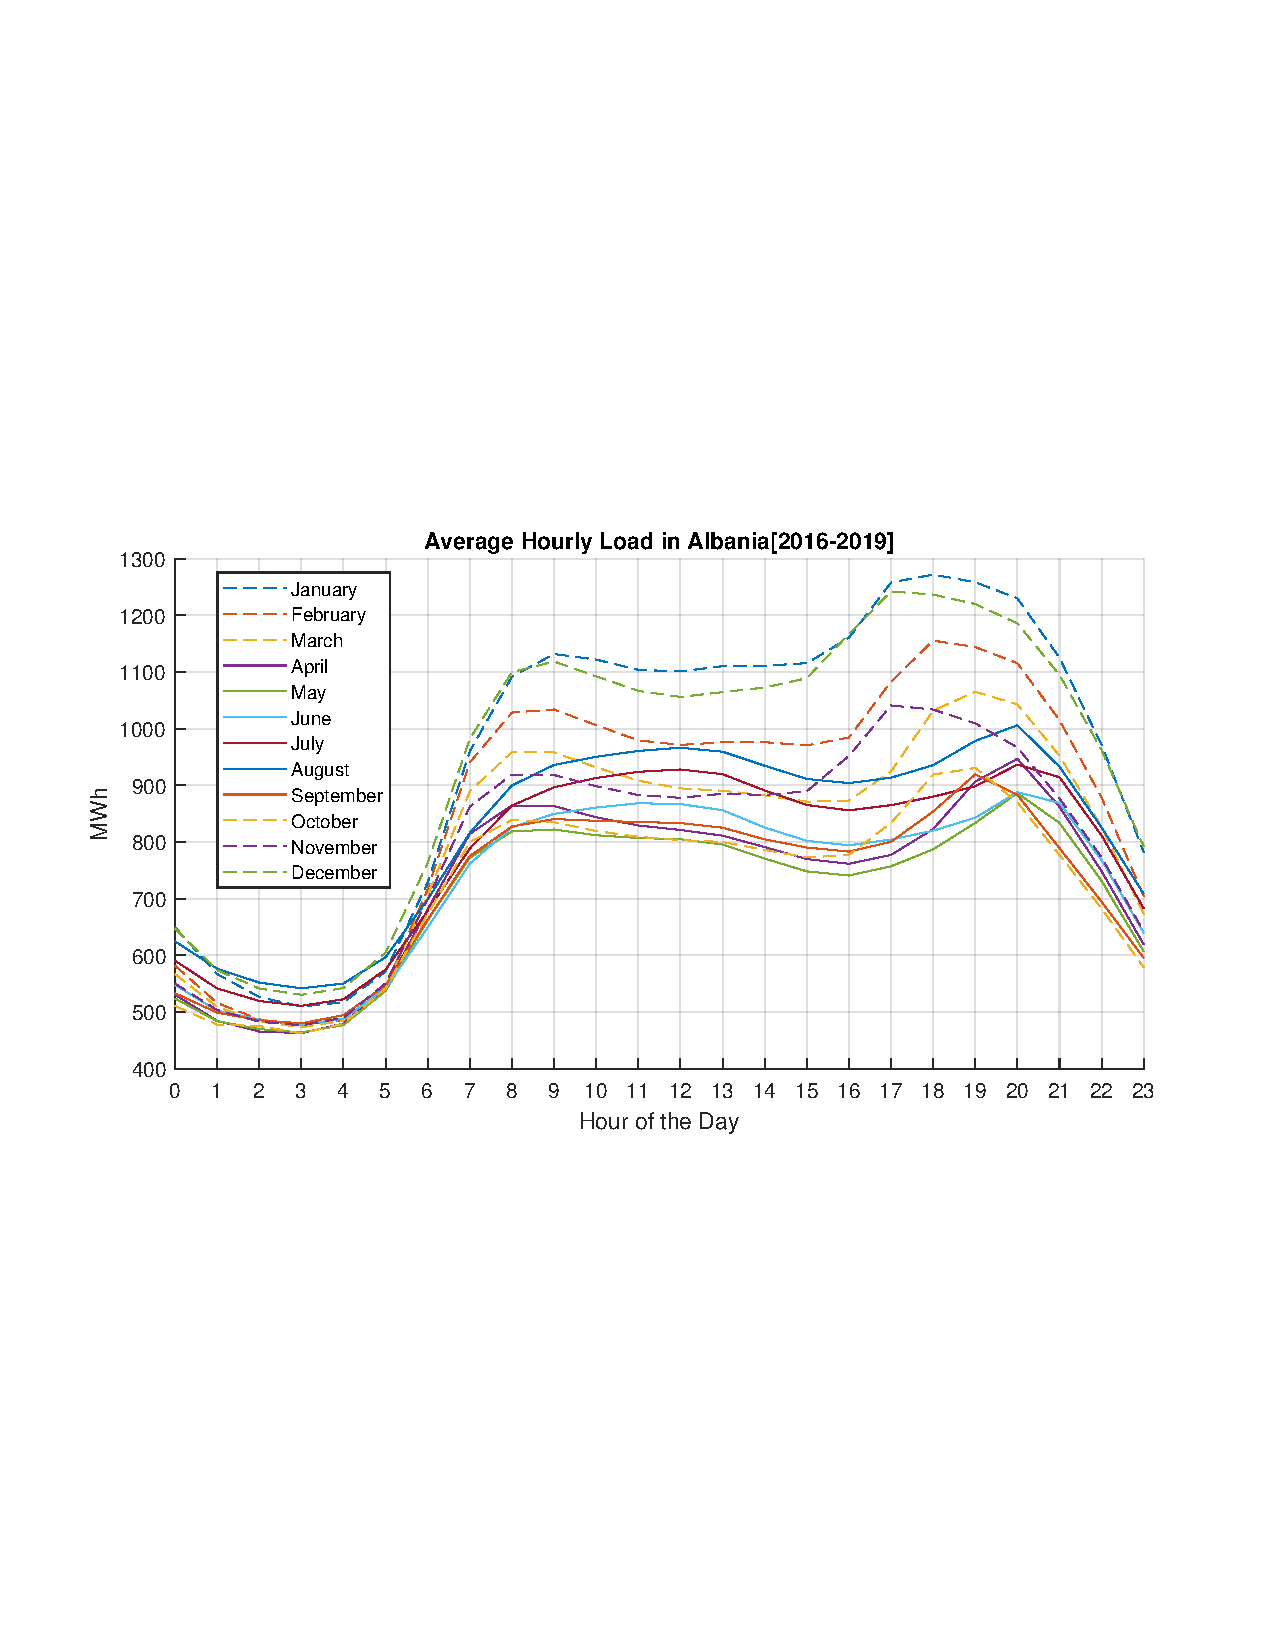
\includegraphics[width=\linewidth]{photos/GridLoadAlbania_2016-2019.pdf}
    \caption{Hourly average of national grid load in Albania from 2016 to 2019. Sorted into average for each month. The winter half-year is dotted to show consumption in these months}
    \label{method:fig:gridloadalbania}
\end{figure}
As mentioned, Albania does not produce much solar power. Meaning this curve will not drop in the midday as the duck curve, and rather flat out. This relationship will change if the household energy mix includes a SHS, as this can produce excess during the day. 

Winter months are consistently higher load than summer months. We can also see a noticeable shift in where the evening peak starts. December and January has their peak at about 17, while summer months peak at 20. The difference is not seen as much in the morning peak. 

\subsection{Daily load profile}
There are three different power settings on the system, and the various systems have different amount of lighting. As mentioned in table \ref{table:product_specifications}, the systems vary from 360 to 1400 lumen based on power setting. The larger system has more light modules that can be connected than the smaller systems. In table \ref{table:light_inventory} we see the inventory of each system. 

%% husk å legg inn hvor lenge de holder i timer for hver setting
\begin{table}[h]
\centering
\begin{tabularx}{\textwidth}{|X|S[table-format=3.1]|S[table-format=3.1]|S[table-format=3.1]|S[table-format=3.1]|S[table-format=3.1]|}
\hline
\textbf{System} & \textbf{Fixed-focus lamps} & \textbf{Tube lights}  &\textbf{USB-A}& \textbf{Min [lm]} & \textbf{Max  [lm]} \\ \hline
BH 300                &               3              &          0    & 2     & 30    & 360 \\ \hline
BH 600                &              3                  &          1   & 2    &   230 & 760 \\ \hline
BH 800                &              3                  &         2    & 2    & 520  & 1400 \\ \hline
\end{tabularx}
\caption{Light module inventory of systems. \textit{Min [lm]} is when all lights on low power setting, \textit{Max [lm]} is when all lights are on full power setting.}
\label{table:light_inventory}
\end{table}

Depending on the power setting and the amount of light, the systems deliver different lumen. Achieving higher lumen at higher power consumption. Table \ref{table:power_configurations_all_systems} shows the consumption for different scenarios in the systems. Power setting, amount of lights and charging via USB all change the power consumption. 

\begin{table}[h!]
\centering
\small % Applied to the whole table float
% Main caption for the entire set of subtables
\caption{Power consumption for BH systems under various operational configurations. Each sub-table details scenarios for a specific system. Systems $S_3, S_6, S_8$ correspond to BH 300, BH 600, and BH 800 and their inventory from Table \ref{table:light_inventory}. Columns \textit{Fixed}, \textit{Tube} and \textit{USB} indicate the number of active components. \textit{Power Setting} shows which power settings the lights are on, $P_L$ (low), $P_M$ (medium), $P_H$ (high). $P_F$, $P_t$ and $P_U$ correspond to the power consumption from \textit{Fixed}, \textit{Tube} and \textit{USB}. $P_{total}$ is the combined power consumption.}
\label{table:power_configurations_all_systems}
\begin{subtable}{\textwidth}
    \centering
    \begin{tabularx}{\linewidth}{|C|S[table-format=1.0]|S[table-format=1.0]|S[table-format=1.0]|C|S[table-format=4.0]|S[table-format=4.0]|S[table-format=5.0]|c|}
    \hline
    \textbf{System} & \textbf{Fixed} & \textbf{Tube} & \textbf{USB} & \textbf{Power Setting} & \textbf{$P_F$ [mW]} & \textbf{$P_T$ [mW]} & \textbf{$P_U$ [mW]} & \textbf{$P_{total}$ [mW]} \\ \hline
    % Data for System S3 (BH 300)
    $S_3$  & 1   & 0   & 0   & $P_L$         & 348        & 0          & 0          & \cellcolor{LightGray}348             \\ \hline
    $S_3$  & 3   & 0   & 0   & $P_H$         & 5760       & 0          & 0          & \cellcolor{LightGray}5760            \\ \hline
    $S_3$  & 2   & 0   & 0   & $P_L$         & 696        & 0          & 0          & \cellcolor{LightGray}696             \\ \hline
    $S_3$  & 3   & 0   & 0   & $P_L$         & 1044       & 0          & 0          & \cellcolor{LightGray}1044            \\ \hline
    $S_3$  & 3   & 0   & 0   & $P_M$         & 2808       & 0          & 0          & \cellcolor{LightGray}2808            \\ \hline
    $S_3$  & 3   & 0   & 1   & $P_L$         & 1044       & 0          & 5000       & \cellcolor{LightGray}6044            \\ \hline
    $S_3$  & 3   & 0   & 2   & $P_H$         & 5760       & 0          & 10000      & \cellcolor{LightGray}15760           \\ \hline
    \end{tabularx}
    \caption{System $S_3$ configurations}
    \label{subtable:power_s3}
\end{subtable}
\vspace{1em} % Adds a little vertical space between subtables
\begin{subtable}{\textwidth}
    \centering
    \begin{tabularx}{\linewidth}{|C|S[table-format=1.0]|S[table-format=1.0]|S[table-format=1.0]|C|S[table-format=4.0]|S[table-format=4.0]|S[table-format=5.0]|c|}
    \hline
    \textbf{System} & \textbf{Fixed} & \textbf{Tube} & \textbf{USB} & \textbf{Power Setting} & \textbf{$P_F$ [mW]} & \textbf{$P_T$ [mW]} & \textbf{$P_U$ [mW]} & \textbf{$P_{total}$ [mW]} \\ \hline
    % Data for System S6 (BH 600)
    $S_6$  & 1   & 0   & 0   & $P_L$         & 348        & 0          & 0          & \cellcolor{LightGray}348             \\ \hline
    $S_6$  & 3   & 1   & 0   & $P_H$         & 5760       & 4080       & 0          & \cellcolor{LightGray}9840            \\ \hline
    $S_6$  & 0   & 1   & 0   & $P_M$         & 0          & 1920       & 0          & \cellcolor{LightGray}1920            \\ \hline
    $S_6$  & 3   & 1   & 0   & $P_L$         & 1044       & 0          & 0          & \cellcolor{LightGray}1044            \\ \hline
    $S_6$  & 3   & 1   & 0   & $P_M$         & 2808       & 1920       & 0          & \cellcolor{LightGray}4728            \\ \hline
    $S_6$  & 3   & 1   & 1   & $P_H$         & 5760       & 4080       & 5000   & \cellcolor{LightGray}14840           \\ \hline
    \end{tabularx}
    \caption{System $S_6$ configurations}
    \label{subtable:power_s6}
\end{subtable}
\vspace{1em} % Adds a little vertical space
\begin{subtable}{\textwidth}
    \centering
    \begin{tabularx}{\linewidth}{|C|S[table-format=1.0]|S[table-format=1.0]|S[table-format=1.0]|C|S[table-format=4.0]|S[table-format=4.0]|S[table-format=5.0]|c|}
    \hline
    \textbf{System} & \textbf{Fixed} & \textbf{Tube} & \textbf{USB} & \textbf{Power Setting} & \textbf{$P_F$ [mW]} & \textbf{$P_T$ [mW]} & \textbf{$P_U$ [mW]} & \textbf{$P_{total}$ [mW]} \\ \hline
    % Data for System S8 (BH 800)
    $S_8$  & 1   & 0   & 0   & $P_L$         & 348        & 0          & 0          & \cellcolor{LightGray}348             \\ \hline
    $S_8$  & 3   & 2   & 0   & $P_H$         & 5760       & 8160       & 0          & \cellcolor{LightGray}13920           \\ \hline
    $S_8$  & 0   & 1   & 0   & $P_M$         & 0          & 1920       & 0          & \cellcolor{LightGray}1920            \\ \hline
    $S_8$  & 3   & 2   & 0   & $P_L$         & 1044       & 0          & 0          & \cellcolor{LightGray}1044            \\ \hline
    $S_8$  & 3   & 2   & 0   & $P_M$         & 2808       & 3840       & 0          & \cellcolor{LightGray}6648            \\ \hline
    $S_8$  & 3   & 2   & 2   & $P_H$         & 5760       & 8160       & 10000      & \cellcolor{LightGray}23920           \\ \hline
    \end{tabularx}
    \caption{System $S_8$ configurations}
    \label{subtable:power_s8}
\end{subtable}
\end{table}

Based on which system the users have, they will have different consumptions for full power or low power. We ask users what power setting they are using, but the information is still not complete. As we choose not to ask about which power setting they are using at which lamp at which time, we miss the complete information of consumption. The missing information will need to be assumed or estimated. 

On the table \ref{table:power_configurations_all_systems} we can see how much energy is used given the power setting and scenario. Knowing the power consumption per scenario and the battery capacity gives us the maximum duration the system can stay in the scenario. We can then compare this to how long they are being in this scenario, to see if the battery will empty. Since we expect seasonal changes to affect the consumption and production, the differences between winter and summer season are large enough to be different cases. We then apply pattern matching in the different outcomes from the cases, like explained in \citep{yinCaseStudyResearch2018}.
\smallskip

Using Matlab, we can create a simple design we have a battery, load and charge to model this system. Matlab also has the possibility of adding a PV module for the system, but we used the data from PVGIS instead. The system is shown in appendix \ref{apx:matlab}, and a test generation is shown in figure \ref{method:fig:method_simulation}. From the figure, we can see how the simulated production and consumption affects the combined charge, which either charges or discharges the battery. 

\begin{figure}[H]
    \centering
    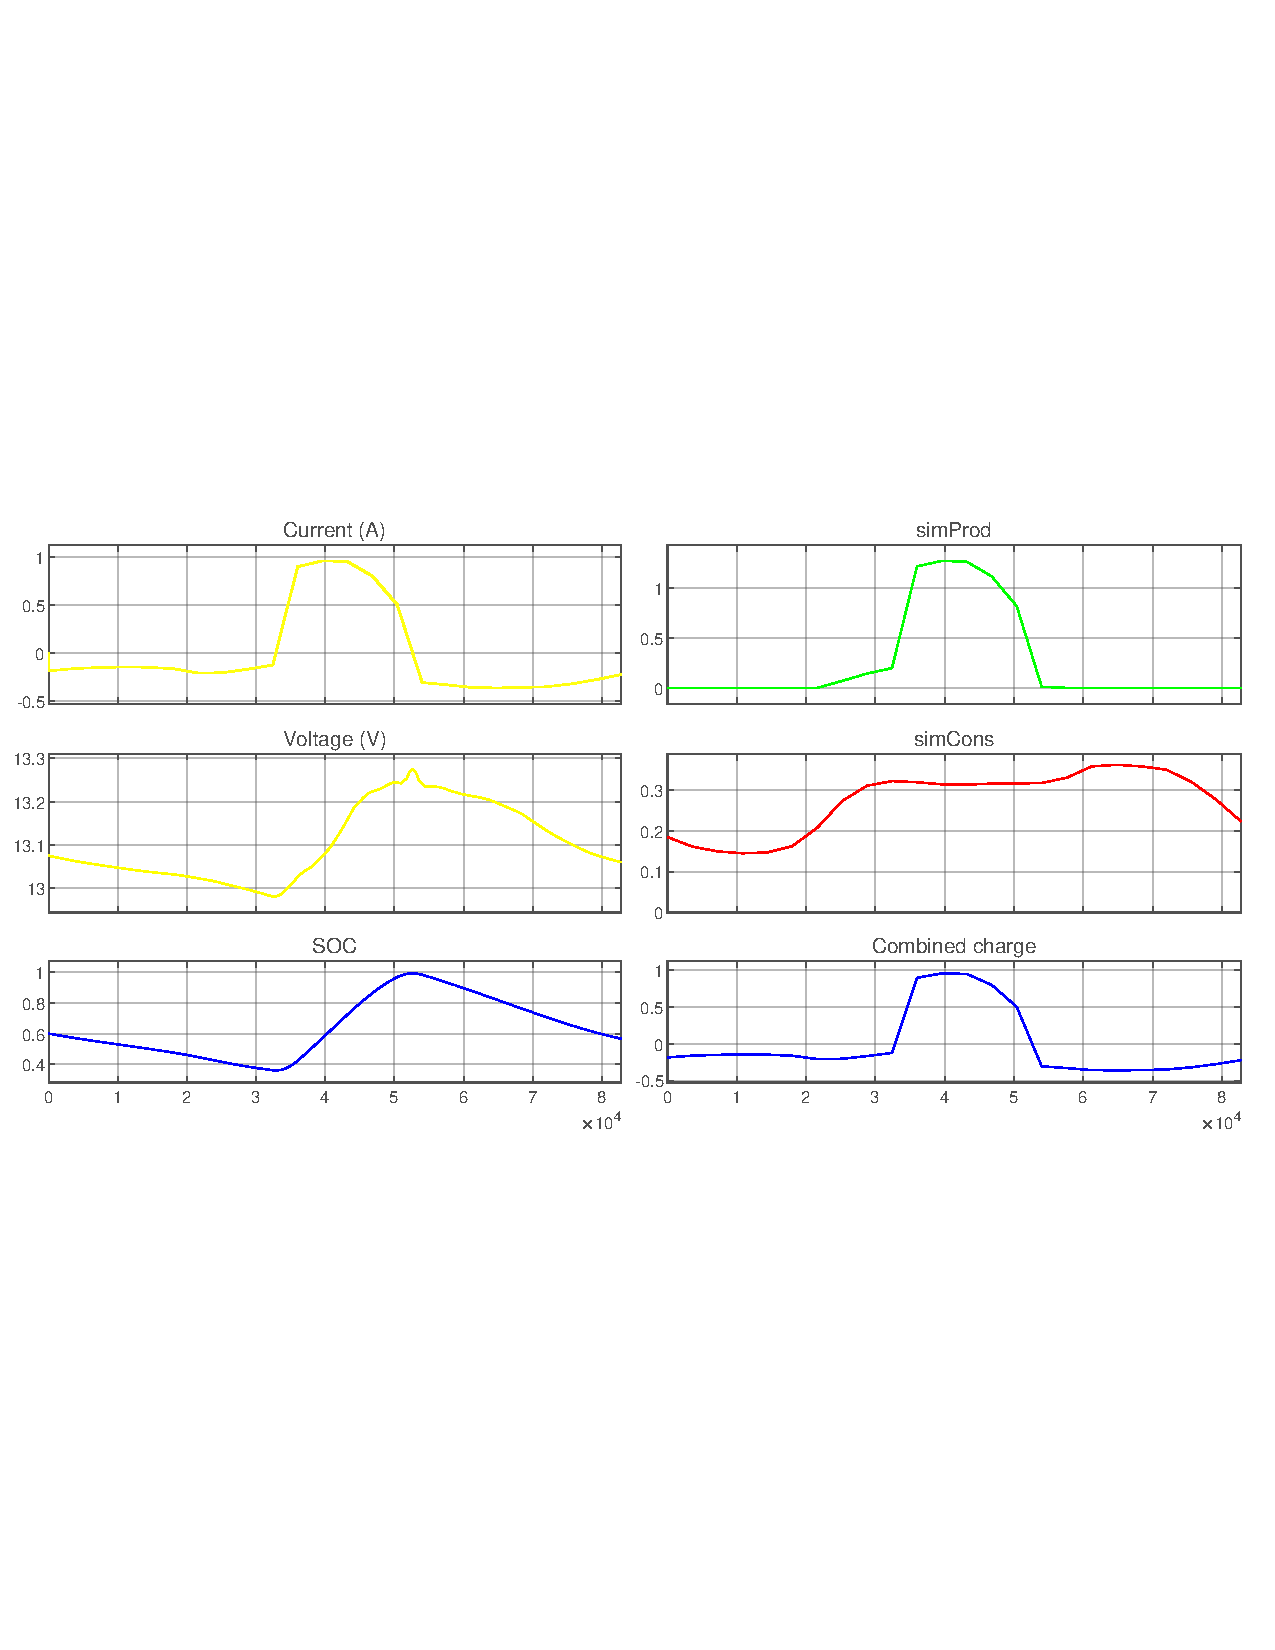
\includegraphics[width=\linewidth]{photos/Method_simulation.pdf}
    \caption{Simulation of how the daily consumption and production would be using an arbitrary value formatted from the national grid load in  figure \ref{method:fig:gridloadalbania}.}
    \label{method:fig:method_simulation}
\end{figure}
In this simulation, the SOC starts and ends at around the same value. Looking at the data from the results, this is an important factor of how well the system will do over time. If the SOC is higher after one 24-hour cycle, than the system is in surplus. If it is lower, than the system will eventually drain into empty. Production for this simulation is taken from January with a BH 800 system. As the graph shows an increase from 0.4 to 1 in SOC, that will not be enough to fully charge the system from empty. This is the factors we will look at in chapter \ref{ch:results}.

To analyze the daily load profile, we asked the questions of how long they are on, what power setting, and when they are on. We asked the same questions for charging from the USB-A port, besides power setting. No data was gathered on how many lamps are on, and if it is Fixed-Focus or Tube light. As we saw from the scenario consumption table \ref{table:power_configurations_all_systems}, this varies a lot for each configuration. Data for this needs to be estimated to create a daily load profile, based on observations and conversation in interviews. 

\subsection{Confidence intervals}
With a small set of data points, the \acrfull{ci} explains the uncertainty we are dealing with. \citep{lovasStatistikkUniversiteterOg2018} refers to student-t distribution when the sample size is below 30. We can apply confidence intervals for the consumption data gathered from the interviews. For consumption data we compare the hourly data points for each of the systems. Creating a point estimator for the standard deviation($s$) and the mean($\bar{x}$). These data will give us the indication of the uncertainty of the data. The reason to not do this with production data, is that the data points are an estimation. As the data is simulated from one setup, there is no variation in the output. Although we could create a CI based on the weather irregularities, this would be inaccurate as the irradiance mean will change throughout the month. 
\section{Economic metrics}

\subsection{Electricity price}
%Explain where the price was found had how we can forecast the price further
The Albanian Power Exchange has dataset of the spot price during 2024 we can use in our calculations\citep{albanianpowerexchangeDAMAlbania20242025}. In addition, we will ask questions of how much a person pays in electricity bills each month to get a rough estimate if that spot price applies for them. From the 2024 report of the Albanian Power Exchange, we get that the mean spot price was 0.112€/KWh. This was an 11,84\% increase from 2023. The report also showed how Albania is importing large amounts of power from Kosovo, being in production deficit themselves. As this power exchange started in 2023, we have no more historical data of the electricity price from this source. 

In figure \ref{method:fig:EU27_elecprice}, we can see how the Albanian electricity price compares to the average for EU-27. The data of the price is in \acrfull{euro}, although Albanians pay in \acrfull{lek}. 

\begin{figure}[H]
    \centering
    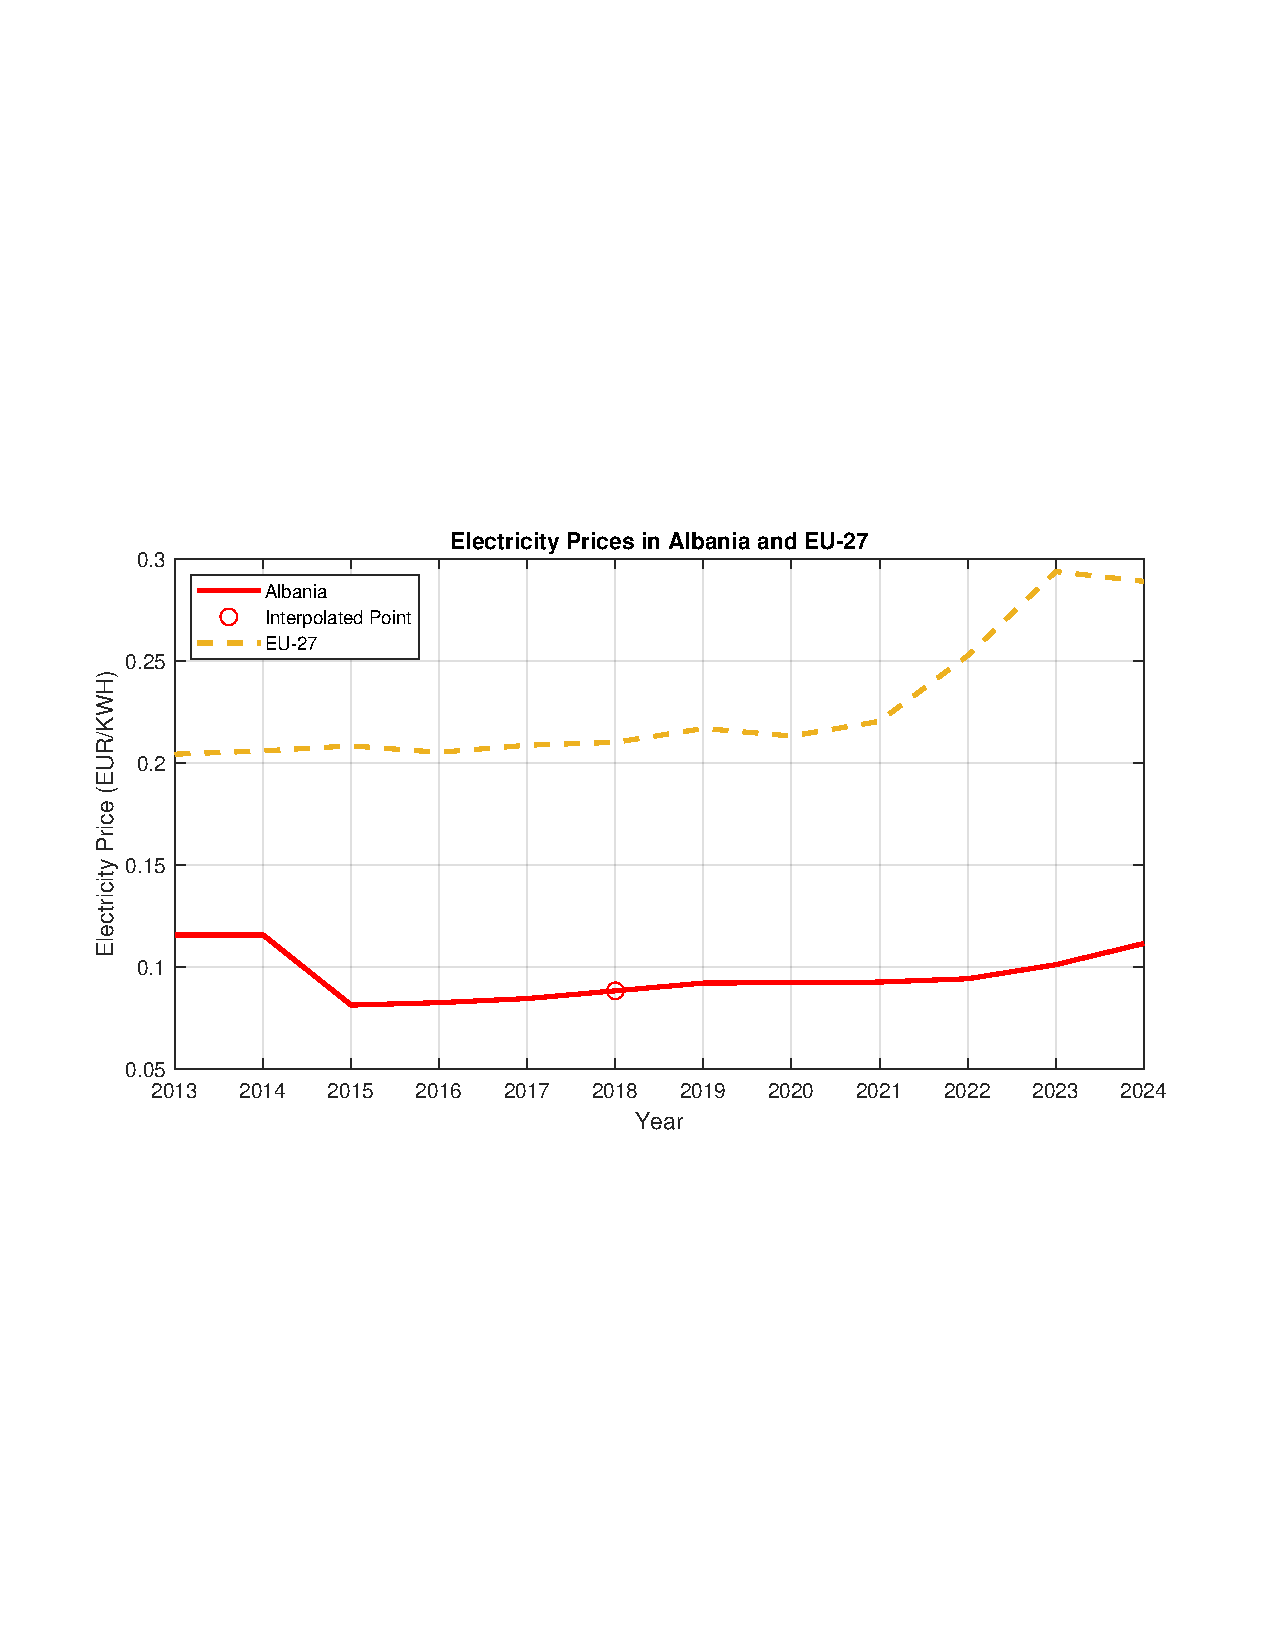
\includegraphics[width=\linewidth]{photos/EU27Electricity_Prices.pdf}
    \caption{One interpolated point due to lack of data in 2018. Data is for a medium size household\citep{eurostatElectricityPricesType2022}}
    \label{method:fig:EU27_elecprice}
\end{figure}

The electricity price for Albanians have been lower than EU-27, but has had a significant rise in the latest years.


Albania charges a fixed price for their electricity per kWh to households, not the spot price they pay for imports. This price will be decreased for household using below \SI{700}{\kilo\watt\hour} per month from 9,5 \acrshort{lek} to 8,5 \acrshort{lek}\citep{euronewsalbaniaImplementationNewElectricity2025}. The price increase in figure \ref{method:fig:EU27_elecprice} is due to the currencies changing in value. Due to the price being relatively stable, and the life cycle being only 7 years, we will not create an electricity forecast for the price. 

\subsection{SHS cost}
Participants of the project was given their system for free. This means that there are two different points of view to take for analysis of the cost of the systems. Either lifetime costs without the investment cost, or lifetime costs with investment cost. Although the product is not sold by Bright Products on the commercial market, third-party retailers sell the product. 

\begin{table}[h]
\centering
\begin{tabularx}{\textwidth}{|X|X|X|}
\hline
\textbf{System} & \textbf{Third-party retail price[EUR]} & \textbf{Bright quantity price[USD]} \\ \hline
BH 300        &  275 & 124 \\ \hline
BH 600        &  367 & 160 \\ \hline
BH 800        &  468 & 222 \\ \hline
\end{tabularx}
\caption{Light module inventory of systems. \textit{Min [lm]} is when all lights on low power setting, \textit{Max [lm]} is when all lights are on full power setting.}
\label{table:SHS_cost}
\end{table}

The lifetime of this system is given in 6-7 years or 2000 charge cycles\footnote{A charge cycle of the battery is defined as it discharging from full to empty, and back up to full.}. There is no more maintenance required to fulfill the given lifetime. Apart from possible malfunction and replacement of the malfunctioning parts, there are no planned costs of owning the SHS.

We also included the question of \textit{What would be a fair price for this system?} in our field trip questions \ref{apx:ftquestions}. The intention of this question was to reveal what the product would have to be priced at for the participants to buy this. Answering if the participants would be able to afford this system at all, or at least how much each participant would be able to share the cost of the system.

\subsection{Levelized Cost of Energy}
\label{chap:method:sec:LCOE}
To evaluate the \acrshort{lcoe}, we will take the cost of buying the product from either Third-party or in quantity from Bright. Lifetime is assumed to be either 2000 charge cycles or 6 to 7 years. As $\frac{2000}{365.25} \approx 5.5$, the lifetime will be based on cycles if the system does one charge cycle each day continuously throughout it's lifetime. Solar panels are expected to last 25-30 years, although \citep{sodhiEconomicLifetimesSolar2022} claims that their realistic lifetime will be shorter based on reduced efficiency. Battery is the bottleneck that Bright refers to for the lifetime of the system. \citep{pregerDegradationCommercialLithiumIon2020} found that \acrfull{lfp} can last up to 9000 cycles before going to 80\% of initial capacity. FLP is the battery type in all of the systems from Bright.


Table \ref{table:cost_per_system} shows the cost of a system per year for the entire lifetime. The lifetime used is based on the minimum expected lifetime, given lifetime from specifications, and the maximum amount of lifetime for the battery. This is all given that the battery will complete a charge cycle each day throughout it's lifetime. 

\begin{table}[H]
\centering
\small
\begin{tabularx}{0.3\textwidth}{|>{\RaggedRight\hsize=0.4\hsize}X|>{\Centering\hsize=0.3\hsize}X|>{\Centering\hsize=0.3\hsize}X|}
\hline
\multicolumn{3}{|c|}{BH 300 System} \\
\hline
\textbf{$C/L$} & \textbf{$C_R$} & \textbf{$C_Q$} \\
\hline
\textbf{$L_{min}$} & 50.2 & 22.6 \\ \hline
\textbf{$L_{6}$} & 45.8 & 20.7 \\ \hline
\textbf{$L_{7}$} & 39.3 & 17.7 \\ \hline
\textbf{$L_{max}$} & 11.2 & 5.0 \\ \hline
\end{tabularx}%
\hspace{0.5em}% Litt horisontal avstand mellom tabellene
\begin{tabularx}{0.3\textwidth}{|>{\RaggedRight\hsize=0.4\hsize}X|>{\Centering\hsize=0.3\hsize}X|>{\Centering\hsize=0.3\hsize}X|}
\hline
\multicolumn{3}{|c|}{BH 600 System} \\
\hline
\textbf{$C/L$} & \textbf{$C_R$} & \textbf{$C_Q$} \\
\hline
\textbf{$L_{min}$} & 67.0 & 29.2 \\ \hline
\textbf{$L_{6}$} & 61.2 & 26.7 \\ \hline
\textbf{$L_{7}$} & 52.4 & 22.9 \\ \hline
\textbf{$L_{max}$} & 14.9 & 6.5 \\ \hline
\end{tabularx}%
\hspace{0.5em}% Litt horisontal avstand mellom tabellene
\begin{tabularx}{0.3\textwidth}{|>{\RaggedRight\hsize=0.4\hsize}X|>{\Centering\hsize=0.3\hsize}X|>{\Centering\hsize=0.3\hsize}X|}
\hline
\multicolumn{3}{|c|}{BH 800 System} \\
\hline
\textbf{$C/L$} & \textbf{$C_R$} & \textbf{$C_Q$} \\
\hline
\textbf{$L_{min}$} & 85.5 & 40.5 \\ \hline
\textbf{$L_{6}$} & 78.0 & 37.0 \\ \hline
\textbf{$L_{7}$} & 66.9 & 31.7 \\ \hline
\textbf{$L_{max}$} & 19.0 & 9.0 \\ \hline
\end{tabularx}
\caption{Cost per year for each system in EUR. Where $L_{min}$ is 2000 charge cycles, $L_{6}$, $L_{7}$ is 6 and 7 years, and $L_{max}$ is 9000 charge cycles. $C_R$ is the retail price, and $C_Q$ is the discounted quantity price.}
\label{table:cost_per_system}
\end{table}

Maintenance costs for the system is not included, but would be expected on a system that has 9000 cycles. Table \ref{table:cost_per_system} also shows how much the system needs to yield each year to be profitable. Comparing this to the amount of electricity produced and consumed from the system, we can see if this system would be a worthwhile investment. If the usage is low on all systems, smaller systems can be more profitable. A BH 300 system only needs to cover €5 of reduced electricity costs a year to be profitable if doing 9000 cycles. 

\subsection{Discount rate}
Using equation \eqref{eq:ramseyformula}, we can find the SDR in equation \eqref{eq:socialdiscountrate}. \citep{internationalmonetaryfundALBANIA2024ARTICLE2025} estimate the long-term real \acrfull{gdp} growth of Albania to about 3.5\%. The pure time preference is set to 0, as we don't have any data on this. $\eta$ is set to 1.5 as the SHS targets low-income households, where increasing consumption is prioritized. 

\begin{align}
    r & =  0 + 1.5\cdot3.5 = \textbf{5.25\%}
    \label{eq:socialdiscountrate}
\end{align}

\citep{inproceedings} used the discount rate of 7\% for a wind farm project in Albania. Being a renewable energy project, it is similar to "Use the Sun". It differs as SHS is a targeted measure towards low-income households, and is primarily humanitarian aid.
\subsection{Payback time}
Using data from table \ref{table:SHS_cost} and the income, we can find the payback time for a system. With data from the question \textit{What do you think a fair price for this product would be if you were to buy it now?} we can compare the actual payback time with what the participants would accept as a payback time. \citep{inproceedings} reported a 7.6 and 8 year payback time for a utility wind farm in Albania. \citep{mannesEnduserEvaluationSolar2017} reported a 44 year payback time for a SHS in South Africa. Theses numbers show that the normal payback time for a SHS is higher than can be expected from a normal investment. \citep{hoqueEvaluationEnergyPayback2014} uses energy yield as a payback indicator based on the CO2 emissions caused by production. They found that in Bangladesh it takes around 7 years for a SHS to produce enough to recover the emissions lost from production. They also assume a 20 year lifespan in the SHS. 

\section{Social}
To analyze the social effects of this project, we needed questions regarding the overall changes this system made to their life. This includes the way they interact with and use the system, how they maintain it, and how their view on solar power systems. Participant's financial situation were generally below average for the area, giving rise to another set of social metrics. How large the cost of electricity is compared to their budget will give a pointer of what impact this system has for them. Households will be of different amount of people, and the use of such a system will benefit more people if the home is more populated. 

\subsection{Power outages}
\label{ch:metod:powerout}
Although Albania has full grid coverage, as mentioned in chapter \ref{ch:intro} - power outages still occur. \citep{nduhuuraImpactsElectricityOutages2021} shows that areas that have full grid coverage still may not have reliable power transmission. The study looks at how power outages in Ghana had diverse outcomes for households, reducing security and increasing food spoilage. Although food spoiling will not be relevant for this small of a system, the increased security will. Asking questions about power outages and their effects will help us do an evaluation of the social benefits participants get. Candles are common as alternative lighting when there is power outages, being a cheap emergency solution. \citep{martyahrensHomeCandleFires2020} shows that in the US, 2\% of home fires and 6\% of home fire injuries are due to candles. Candles are mostly used from decoration in the US, meaning that the use and dangers may be higher in developing countries. 

\subsection{Technology adoption}
Solar power is an old technology, but has not been widely used until recent years. Introducing solar power requires some understanding of the use and functionality of the system. As mentioned in chapter \ref{ch:theory}, angle, azimuth and soling can have a large impact on the efficiency of the panel. As mentioned in chapter \ref{ch:background}, some studies claimed training as a barrier to entry. Although there is a manual with some easy setup steps for the system, getting an optimal use out of the system requires specific knowledge. As the caption from figure \ref{method:fig:wattage_generation_PV40wpp} reveals, the optimal values for this area are not the ones given as a general rule of thumb. An azimuth $\phi=35\degree$ is not the typical $0\degree$ given as standard for the northern hemisphere. As there are many functional tilt angles and azimuths for the panel, we will measure how well each of the different setups work. Comparing it towards the optimal, we can then see if there is a need for better installation training of the systems or if the manual was sufficient. 

\subsection{Solar energy awareness}
One of the project goals was to educate communities about the benefits of solar energy. Showing participants how using solar power can supply them directly with electricity and not supplied from the grid would hopefully encourage to more use of this power source. As mentioned in chapter \ref{ch:background}, Albania has solar ongoing solar energy projects that seek to increase the capacity. We asked the question of \textit{What are your thoughts on solar power as an energy resource?}, intending to get an answer of how receiving the solar panel has affected their thoughts. 


%\input{chapters/eval}
%!TEX root = ../thesis.tex

\chapter{Results}
\label{ch:results}

\section{Production profile}


\subsection{Tilt angle and azimuth}
The loss factors that show to be greatest is the mounting of the panel. Some panels where re-mounted during the interviews, as they were tilted the wrong way for optimal production. Although a lot of them were helped in the placing of the system, the tilt and azimuth varied for each system. Figure \ref{result:fig:slope_efficiency} shows that there is no correlation between the slope efficiency\footnote{The slope efficiency is calculated using a yearly total sum of energy produced with different slopes from \citep{huldNewSolarRadiation2012}} of the panels, and if they were helped or not. The average efficiency loss from the system was 21\%. 

\begin{minipage}[t]{0.5\textwidth} % Adjust width as needed
    \begin{figure}[H]
        \centering
        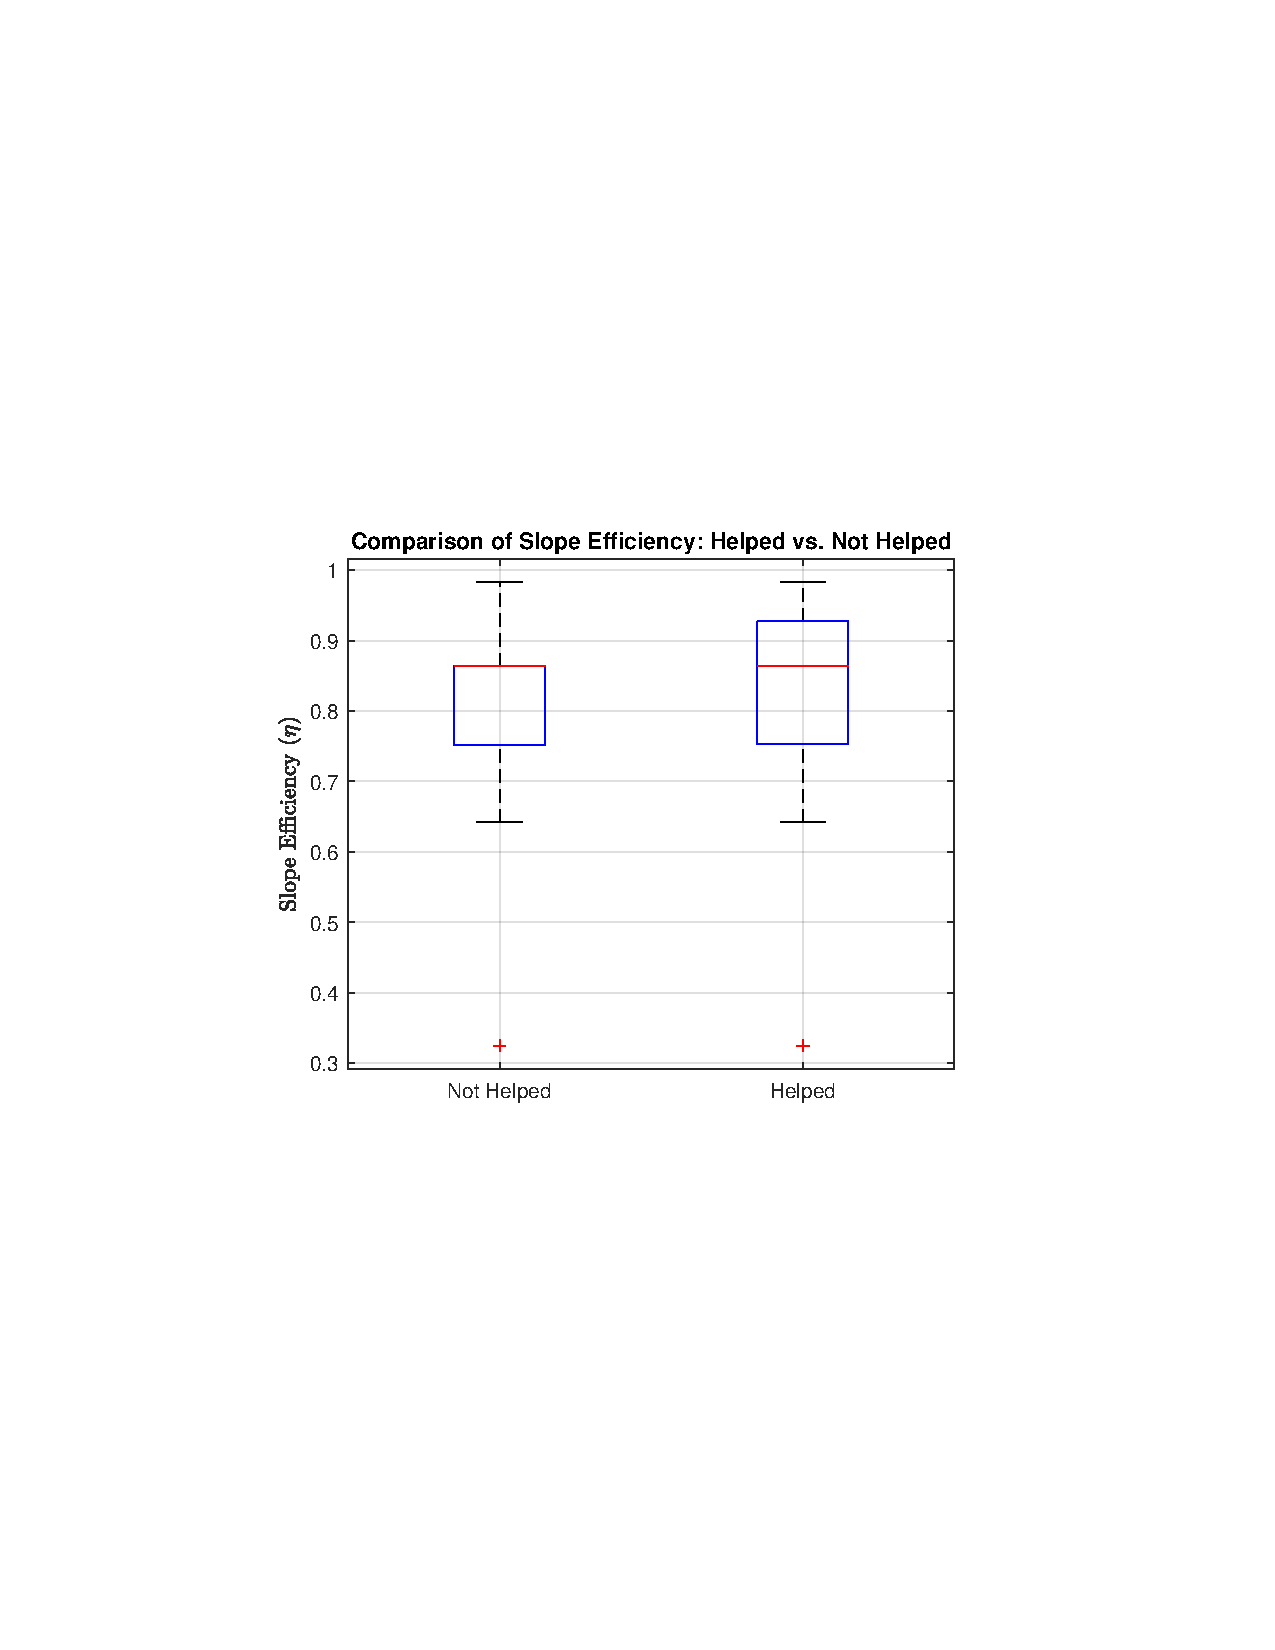
\includegraphics[width=\linewidth]{photos/SlopeEfficiency.pdf} %% Gjer denna om til kryss og sirkel
        \caption{Slope efficiency in a box plot. Red line is the median, the blue box contains the middle 50\% of data points and the red crosses are outliers.}
        \label{result:fig:slope_efficiency}
    \end{figure}
\end{minipage}% <--- IMPORTANT: The '%' symbol prevents unwanted horizontal space
%\hspace{0.01\textwidth}% Adjust this to control the horizontal space between figure and table
\begin{minipage}[t]{0.5\textwidth} % Adjust width so (width1 + hspace + width2) is about 1.0\textwidth
\vspace{0.05\textwidth}
    \begin{table}[H]
        \centering
        \small % To match the font size of your example table
        % Define the new table based on the updated image data
        % The \linewidth here refers to the width of this minipage (0.46\textwidth)
        \begin{tabularx}{\linewidth}{|>{\RaggedRight\arraybackslash\hsize=0.40\hsize}X|>{\Centering\arraybackslash\hsize=0.20\hsize}X|>{\Centering\arraybackslash\hsize=0.20\hsize}X|>{\Centering\arraybackslash\hsize=0.20\hsize}X|}
        \hline
        % Title row for the table (not bold, matching your example's multicolumn style)
        \multicolumn{4}{|c|}{Placement Effectiveness Data} \\
        \hline
        % Column Headers with math mode as requested
        Placement & \textbf{$\phi$} & \textbf{$\alpha$} & \textbf{$\eta$} \\
        \hline
        % Data rows from the new image, in the specified order
        % Assuming "Angled $$S" is "Angled $S$" and "Vertial" is "Vertical"
        % Interpreting "Angled" and "$S_E$" on subsequent lines as "Angled $S_E$"
        Angled $S$ & 0 & 35 & 0.98 \\ \hline
        Angled $S$ & 0 & 45 & 0.97 \\ \hline
        Angled $S_E$ & -45 & 20 & 0.89 \\ \hline
        Horizontal & 0 & 0 & 0.86 \\ \hline
        Angled $S_E$ & -45 & 35 & 0.86 \\ \hline
        Vertical $S$ & 0 & 90 & 0.64 \\ \hline
        Vertical $E$ & -90 & 90 & 0.33 \\ \hline
        \end{tabularx}
        \caption{Effectiveness of different azimuth ($\phi$) and slope ($\alpha$) combinations. ($\eta$) is efficiency where $\eta=1$ is the optima}
        \label{table:placement_effectiveness_data_new} % Choose a new unique label
    \end{table}
\end{minipage}

This could be due to the lack of experience of angle and azimuth from the installers, and perhaps a fear from the participants of changing the setup of the donated system.  

\subsection{Cleaning}
When asked if they had cleaned the panel, only one system was cleaned out of 19 in the study. Most explained that they did not want to touch the panels, as they were afraid to break them. Most panels did not look visibly soiled, and were often placed on roofs away from the dust. The region is not an arid region, and as mentioned in chapter \ref{ch:theory}, it will not be subject to heavy soiling. Although not in a heavy soiling environment, they will still be soiled and need washing to have full effect. As found in chapter \ref{ch:theory}, the soiling in mild regions will cause about a 10\% reduction in efficiency. 

\subsection{Simulation results}
In figure \ref{result:fig:Production_Simulation_results_summer&winter} we see the average production with all loss factors included. The graph shows the difference between the panels for the systems, with their effectiveness range from installation as well. Both duration and peak is significantly lower in the winter season than the summer season, justifying the need for two scenarios. The wide shaded region shows how much the installation process matters for the production of the panel. In general the effectiveness is still high, even though the average has not accounted for low $\eta$ outliers. 
\begin{figure}[H]
    \centering
    \begin{minipage}[t]{0.48\textwidth} % Adjust width as needed
        \centering
        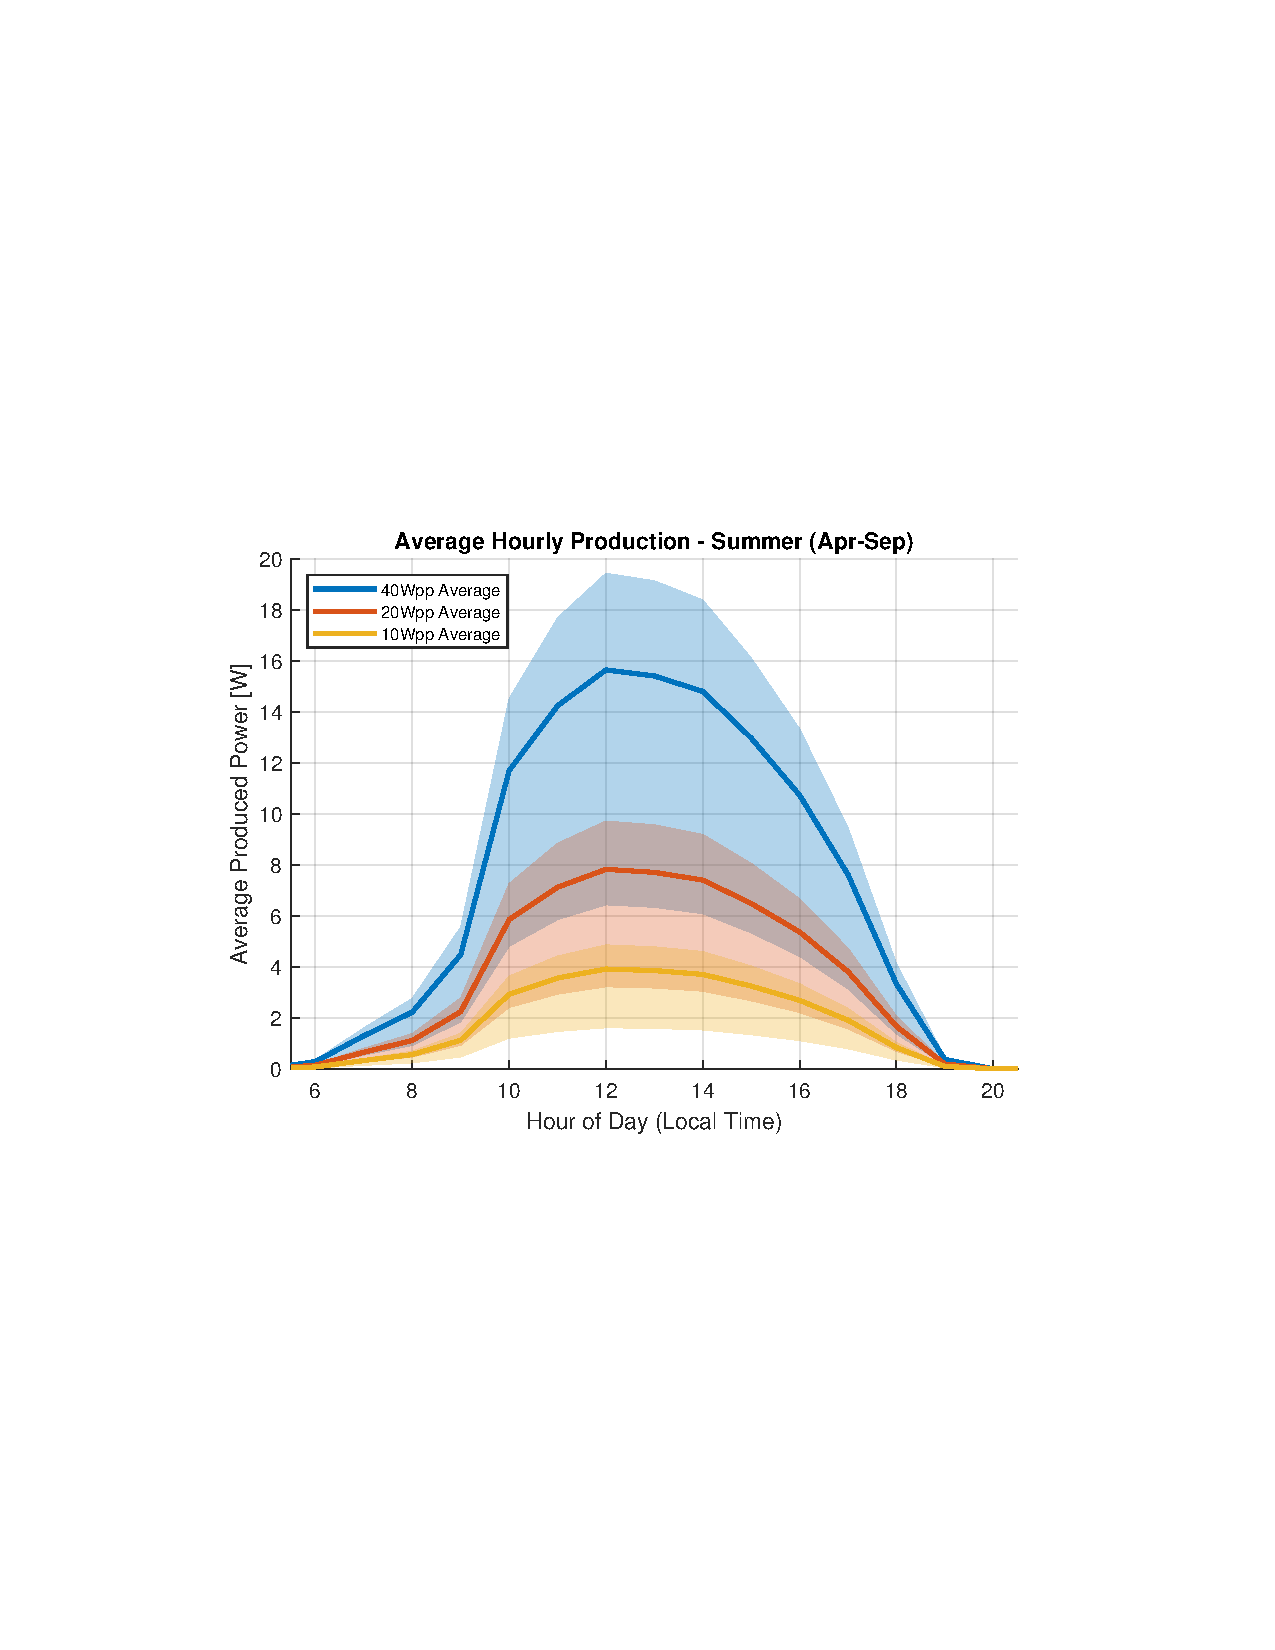
\includegraphics[width=\linewidth]{photos/Average_production_with_eta&soiling&loss_shaded_allPanels_Summer.pdf} %% Gjer denna om til kryss og sirkel
    \end{minipage}%
    \hspace{0.02\textwidth}% Adjust this to control the horizontal space between figure and table
    \begin{minipage}[t]{0.48\textwidth} % Adjust width so (width1 + hspace + width2) is about 1.0\textwidth
        \centering
        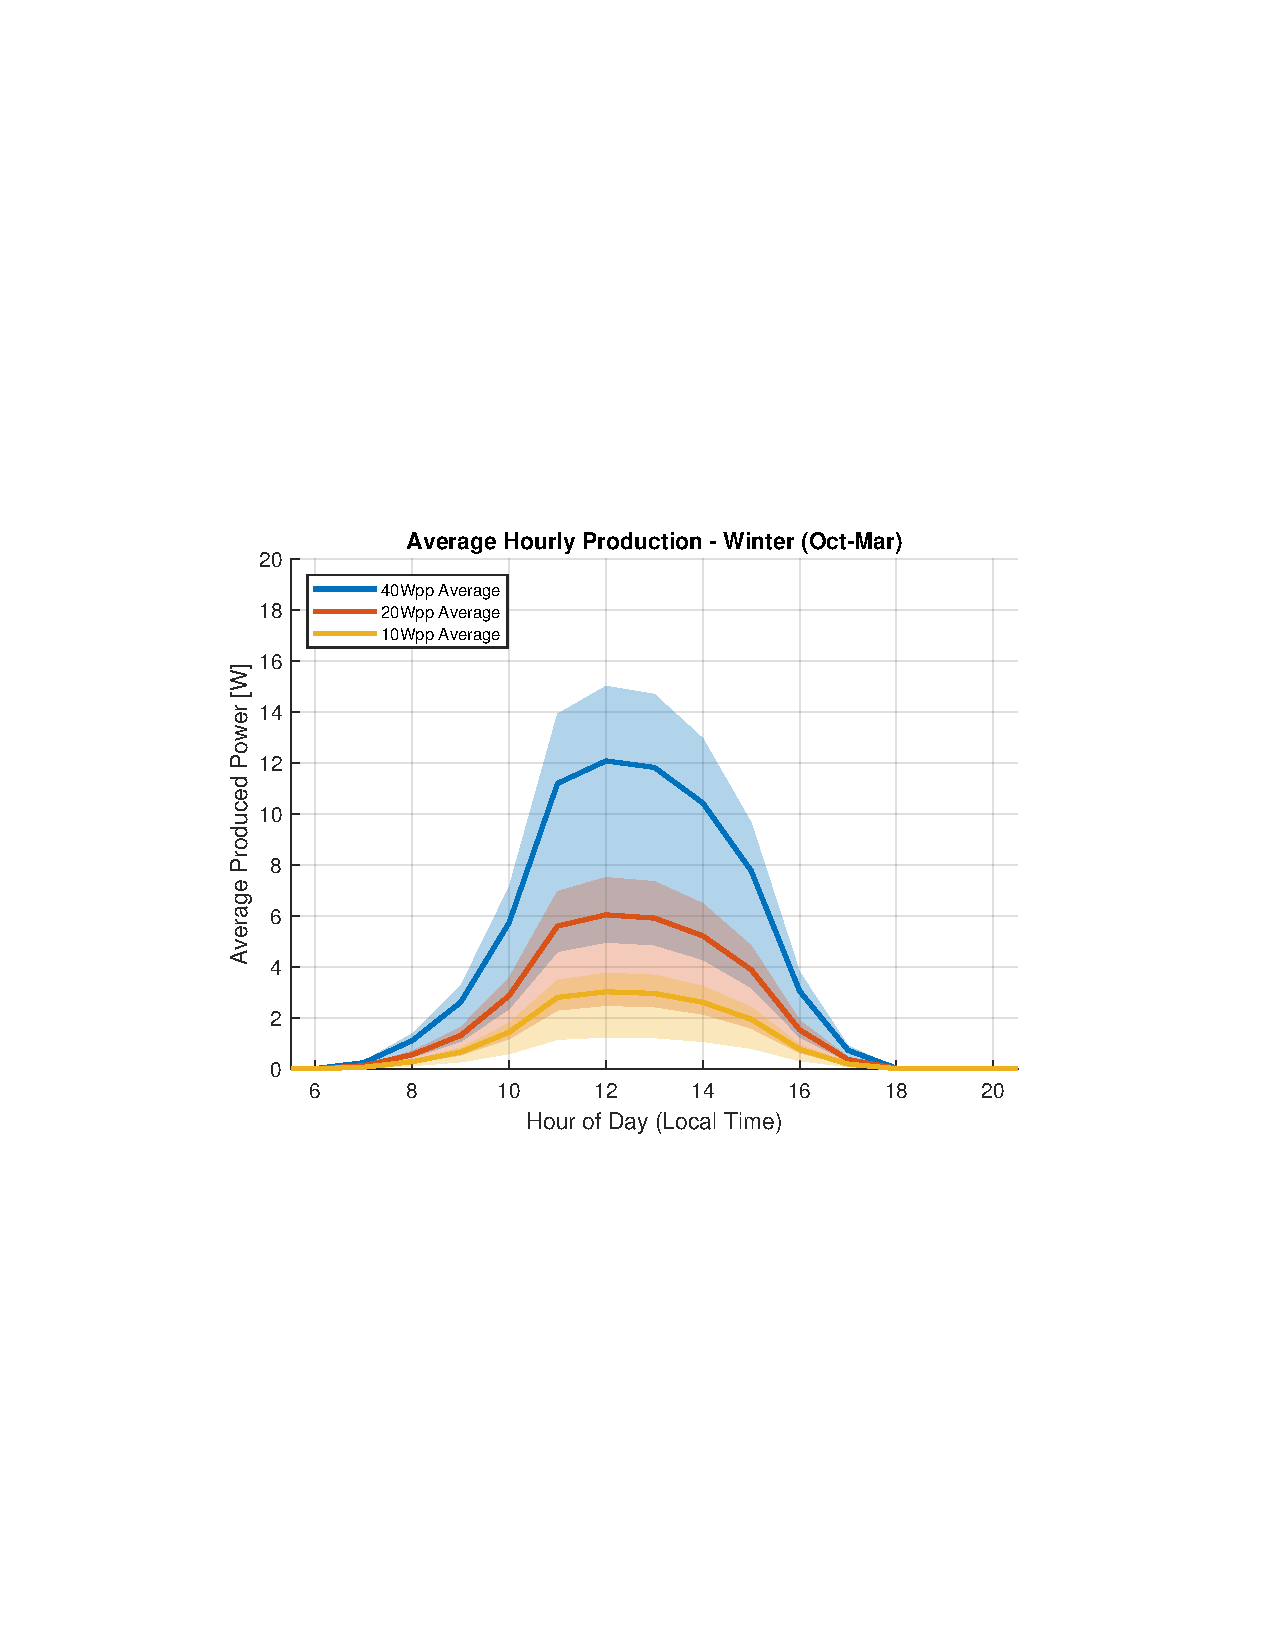
\includegraphics[width=\linewidth]{photos/Average_production_with_eta&soiling&loss_shaded_allPanels_Winter.pdf} %% Gjer denna om til kryss og sirkel
    \end{minipage}
    \caption{Summer and winter average production with loss factors. Soiling 10\%, general transmission loss 14\%. Shaded area represents the area between the most and least effective $\eta$ based on installation, data from table \ref{table:placement_effectiveness_data_new}. The line is the average of the data vectors in the area.}
    \label{result:fig:Production_Simulation_results_summer&winter}
\end{figure}


\section{Daily load profile}
The consumption data for the daily load profile is not as precise as it could be, if there was data logging on the systems. Some of the data needed to be estimated from the interview data and some weather data for sunrise and sunset. We end up with having two different dataset, one for winter and one for summer. These two sets show what we also see from the graph of national consumption on figure \ref{method:fig:gridloadalbania}, that winter months have higher load than summer months. 
\subsection{Consumption profile}
Figure \ref{result:fig:mean_power_allsystems_with95CI} shows the average power drain during 24-hours, derived from the consumption data of all systems. The consumption seems to follow the duck curve referenced in \ref{ch:method}. Having a lower consumption during the midday, when the power generation is highest. Different from the duck curve and the national grid load, the SHS has more load during the night. As the SHS supplies mainly light, this corresponds to the intended usage. 

\begin{figure}[H] % Using [H] as per your code; consider [!htbp] for production
    \centering % Center the entire figure block on the page

    % Left Column: Main Figure
    \begin{subfigure}[t]{0.52\linewidth} 
        \vspace*{0pt} % Ensures the reference point for [t] alignment is the very top
        \centering
        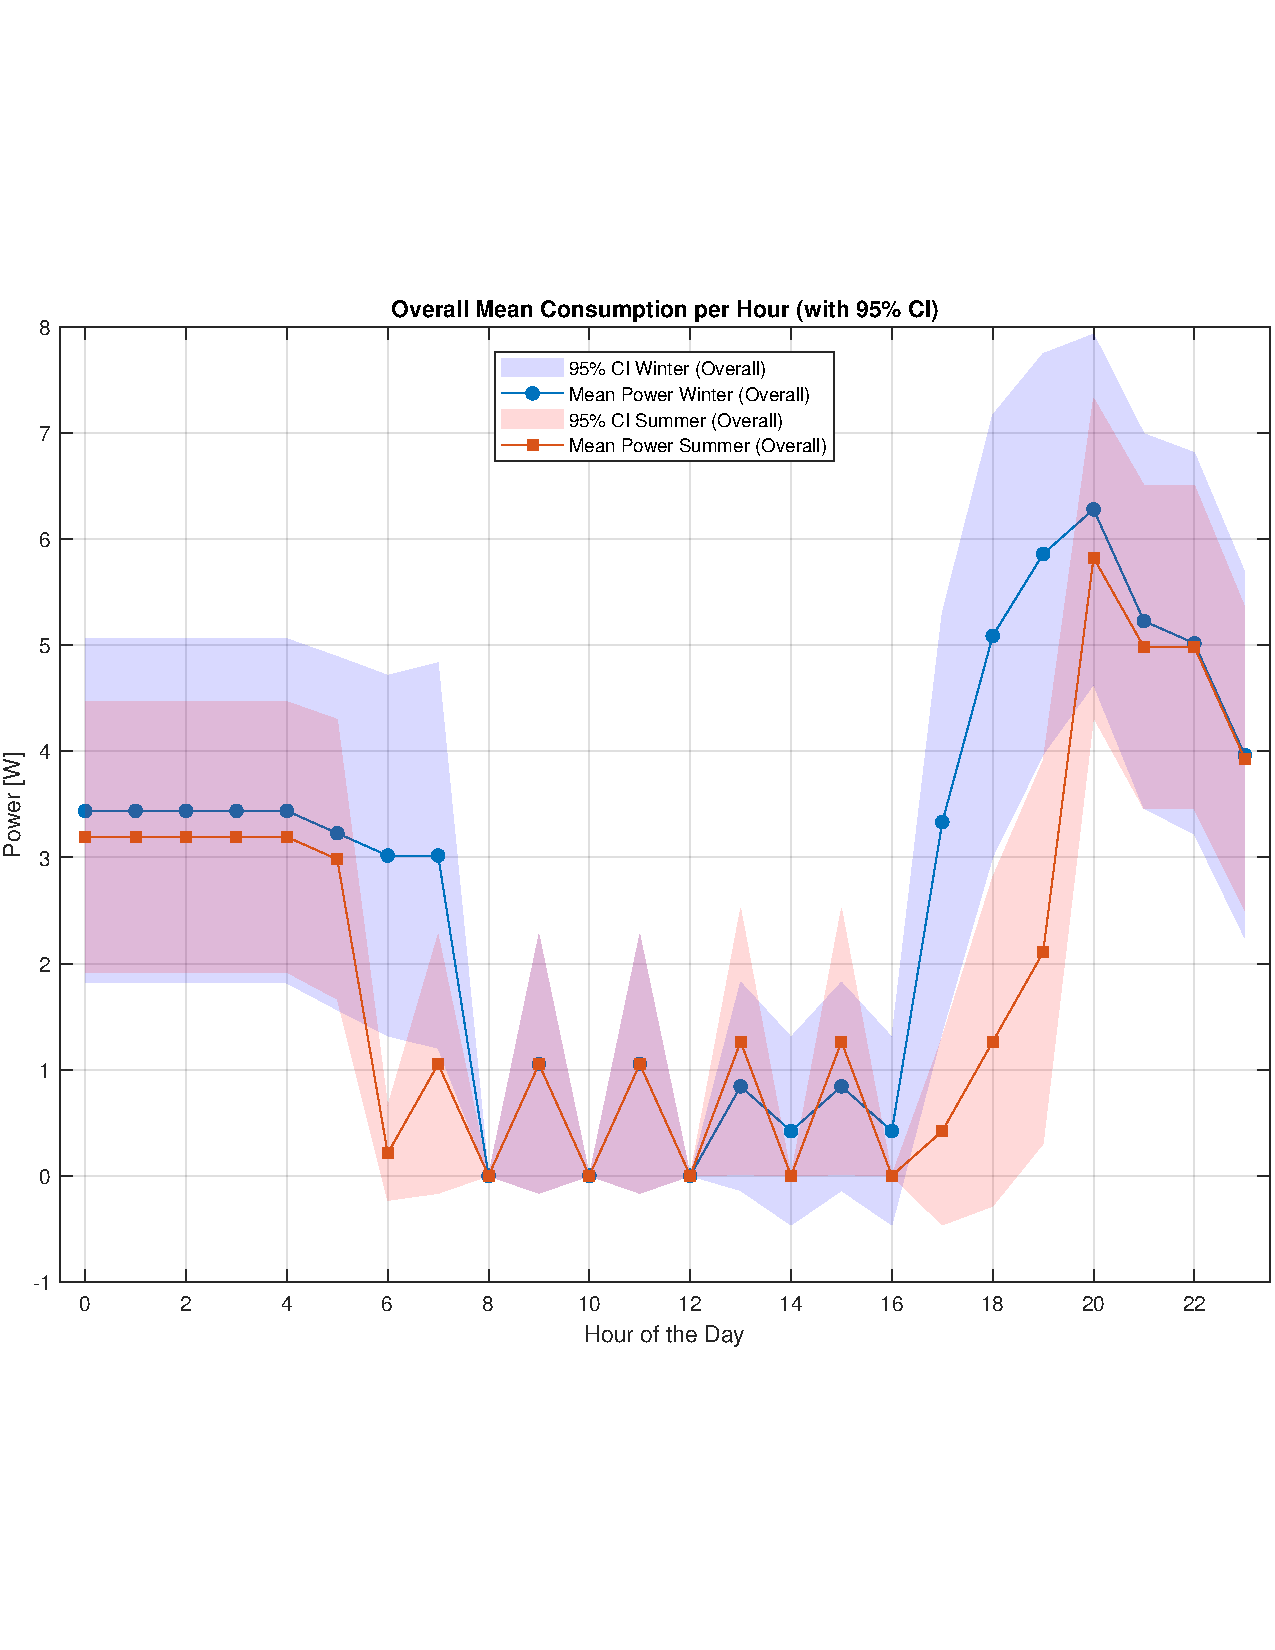
\includegraphics[width=\linewidth, height=\LeftImageHeight, keepaspectratio]{photos/Mean_consumption_winter&summer_all_systems_with_95CI.pdf}
        %\captionsetup{font=footnotesize}
        %\caption{Mean consumption from all systems during summer and winter. 95\% confidence interval applied.}
        %\label{result:fig:mean_power_allsystems_with95CI}
    \end{subfigure}\hfill % \hfill creates a flexible horizontal space
    % Right Column: Stack of Three Figures
    \begin{minipage}[t]{0.45\linewidth} 
        \vspace*{0pt} % Ensures the reference point for [t] alignment is the very top
        \centering 
        \begin{subfigure}{\linewidth} 
            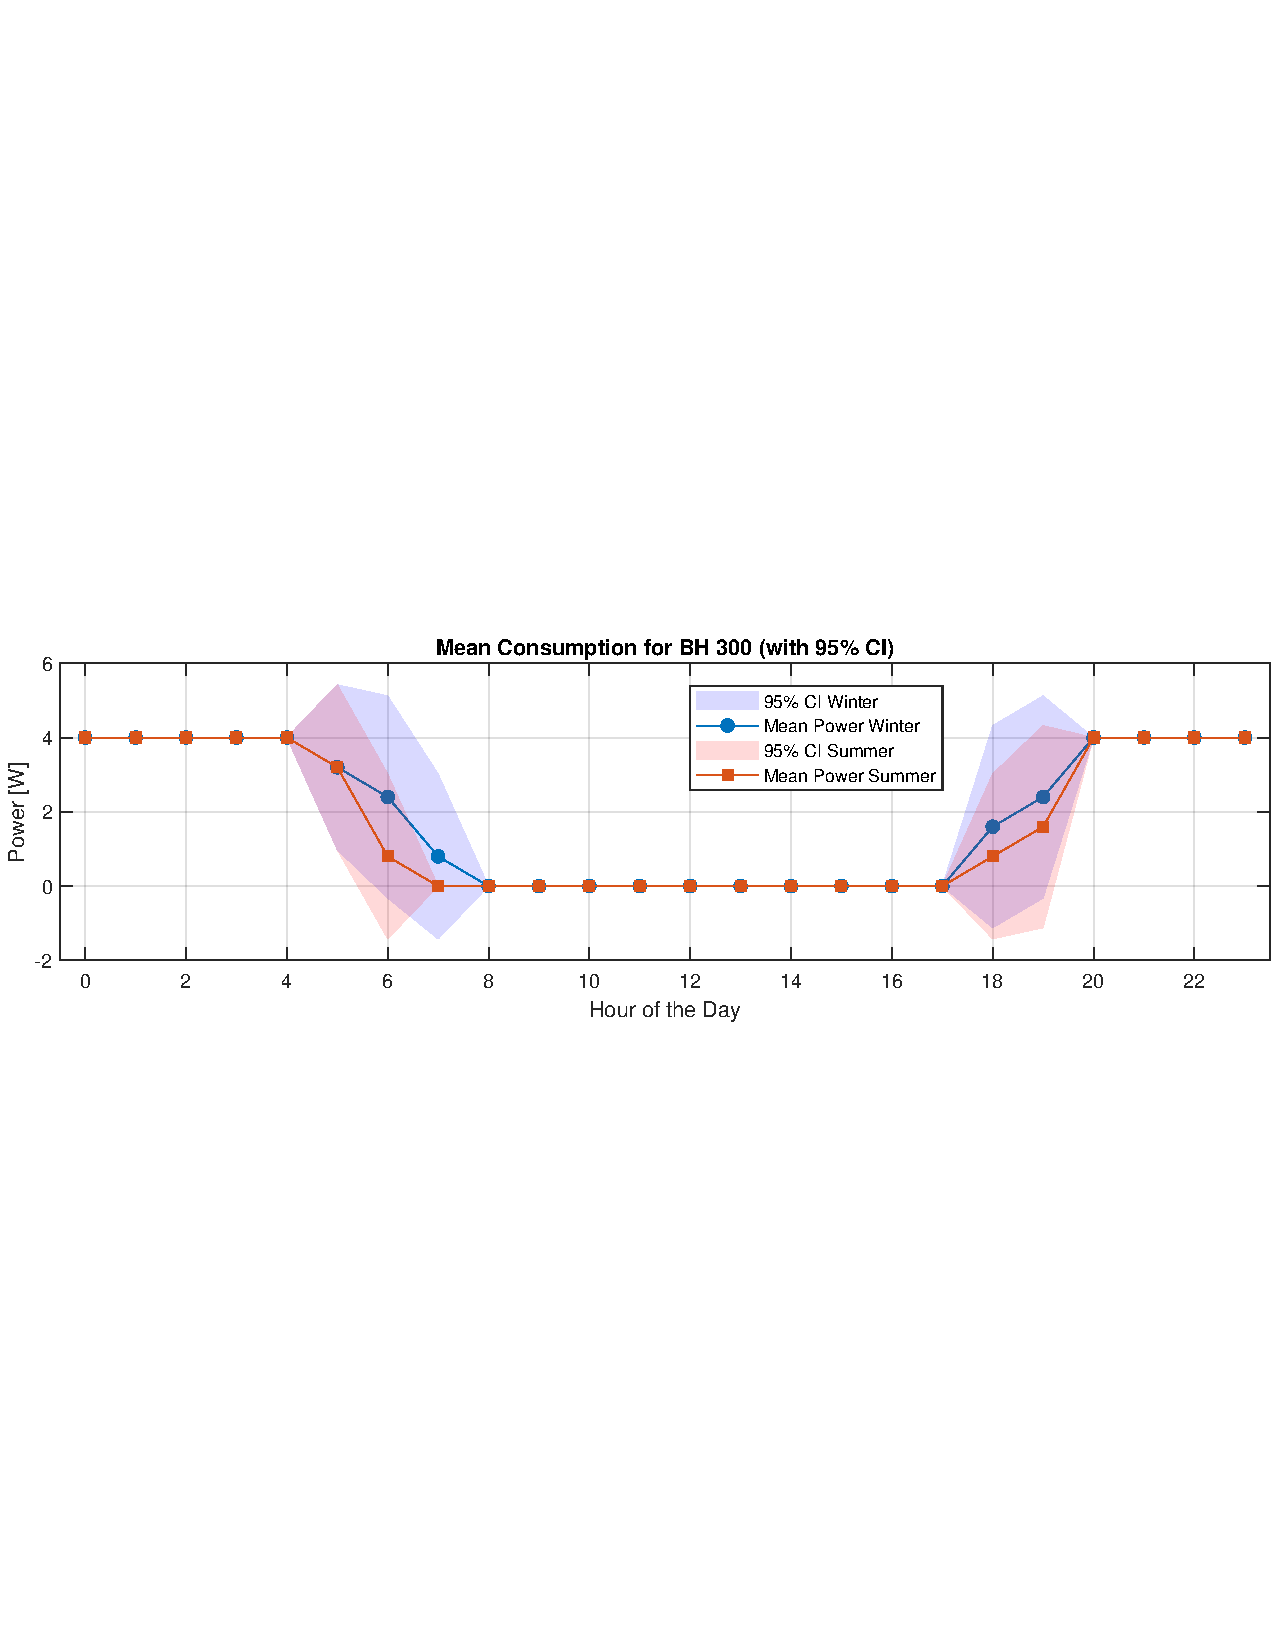
\includegraphics[width=\linewidth, height=\RightImageEachHeight, keepaspectratio]{photos/Mean_consumption_winter&summer_system1_with_95CI.pdf}
            %\captionsetup{font=tiny}
            %\caption{Consumption for System 1 with CI (Example)}
            %\label{fig:system1_CI}
        \end{subfigure}
        \par\vspace{\RightImageVSpace} % \par ensures \vspace is inter-paragraph space if needed
        \begin{subfigure}{\linewidth}
            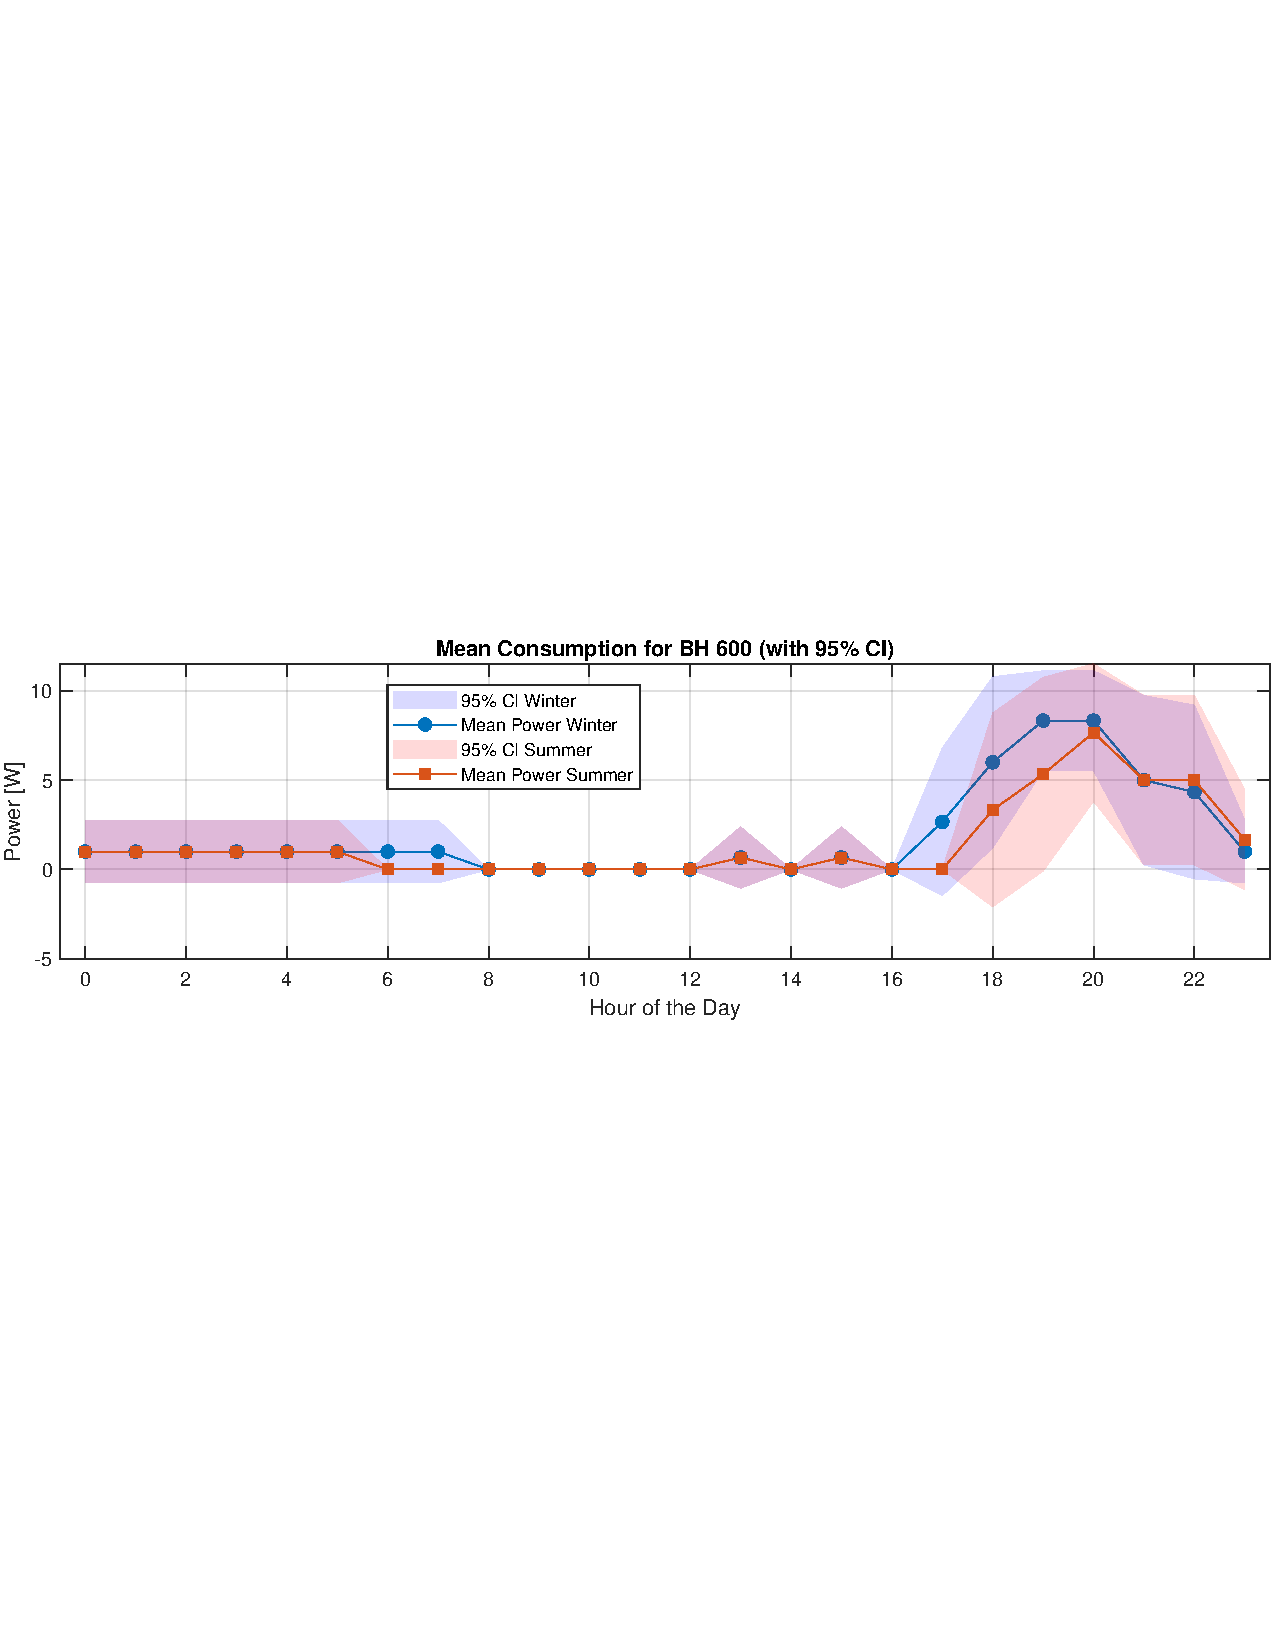
\includegraphics[width=\linewidth, height=\RightImageEachHeight, keepaspectratio]{photos/Mean_consumption_winter&summer_system2_with_95CI.pdf}%\captionsetup{font=tiny}
            %\caption{Consumption for System 2 with CI (Example)}
            %\label{fig:system2_CI}
        \end{subfigure}
        \par\vspace{\RightImageVSpace}
        \begin{subfigure}{\linewidth}
            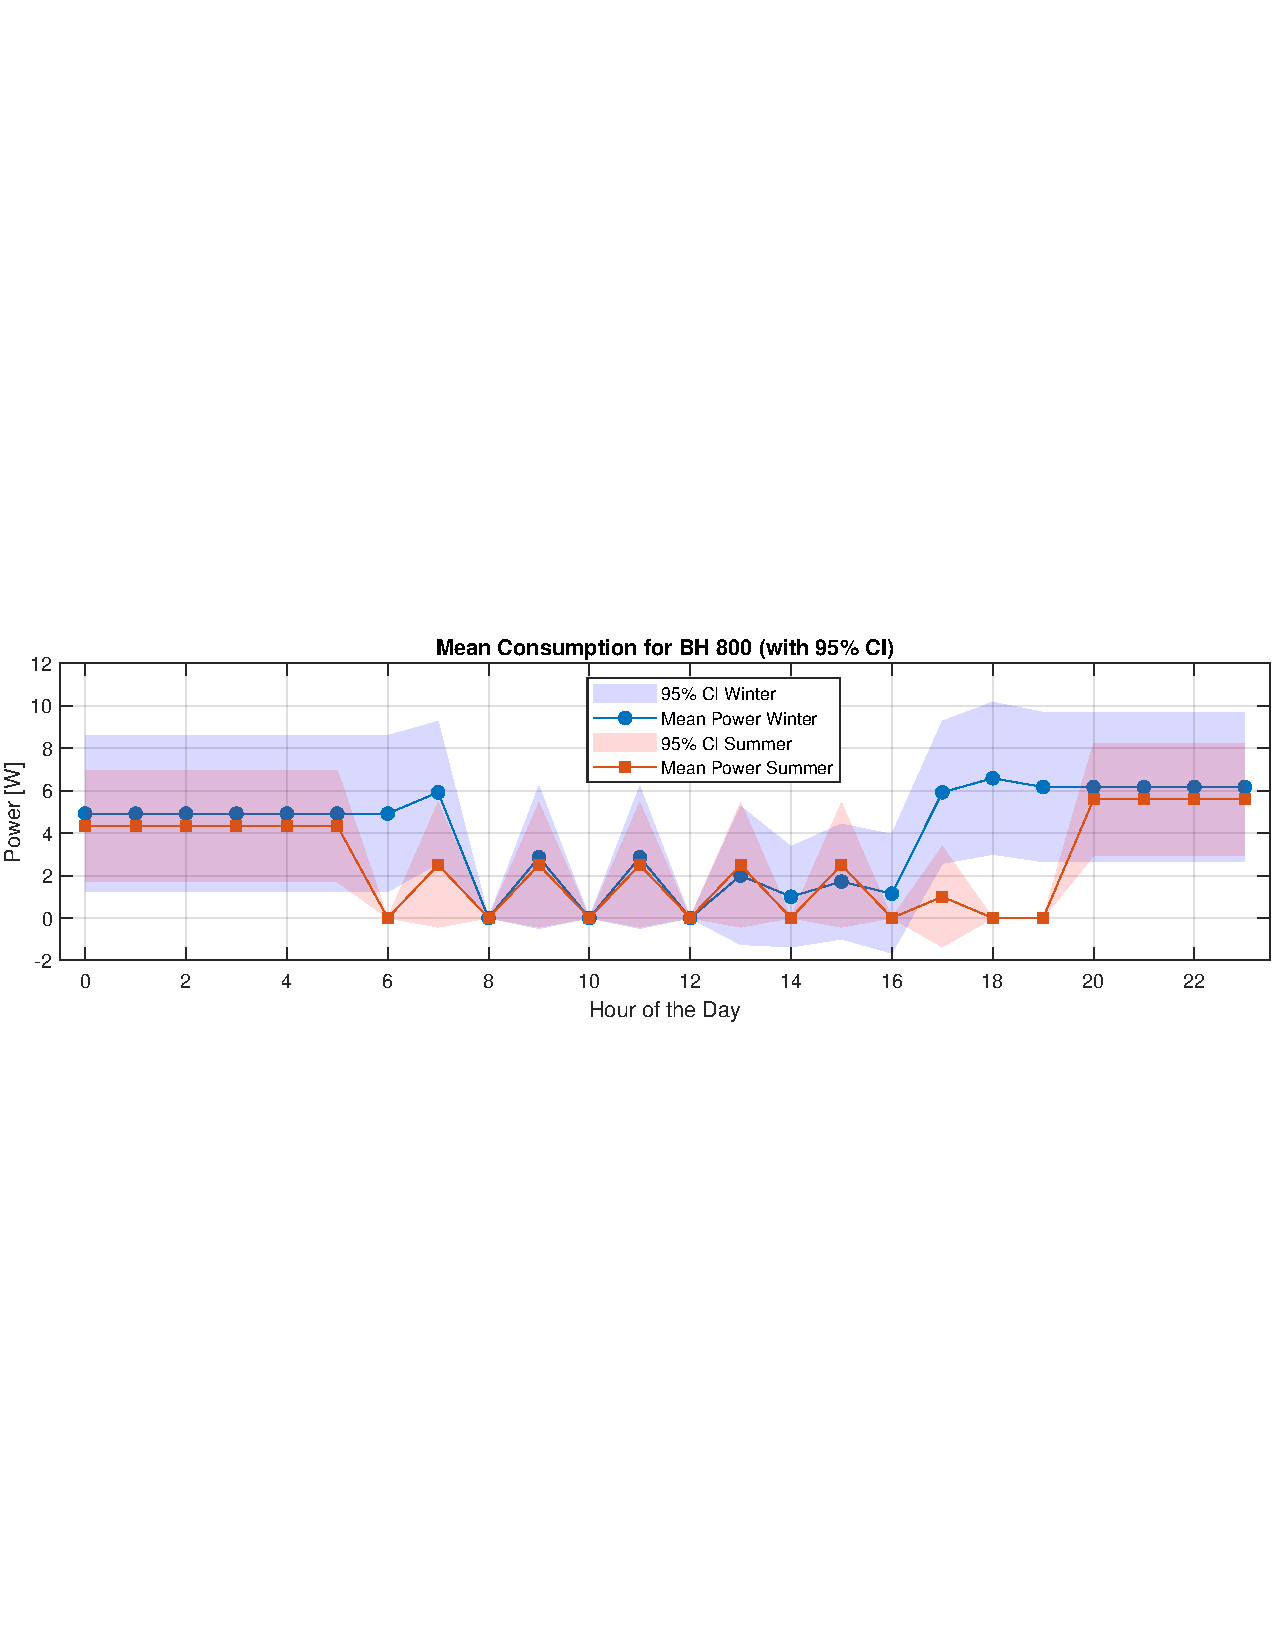
\includegraphics[width=\linewidth, height=\RightImageEachHeight, keepaspectratio]{photos/Mean_consumption_winter&summer_system3_with_95CI.pdf}%\captionsetup{font=tiny}
            %\caption{Consumption for System 3 with CI (Example)}
            %\label{fig:system3_CI}
        \end{subfigure}
    \end{minipage}
    \caption{Mean consumption from all systems during summer and winter. 95\% confidence interval applied. The left figure is for all systems combined with sample size $n=19$, and the right figures are for each system individually. BH 300, BH 600 and BH 800 has respectively $n=5$, $n=6$ and $n=8$ samples.} 
    \label{result:fig:mean_power_allsystems_with95CI}
\end{figure}
Summer and winter mostly differs in regards to when the power peak starts in the evening, and when it stops in the morning. The actual power peak and following consumption pattern matches for both winter and summer data. Using a low sample can give inaccurate data. From figure \ref{result:fig:mean_power_allsystems_with95CI} in the top right for BH 300, we have a small CI for the data. Having a low sample size with no variation, it seems to be more accurate than it is. Using a consumption profile for all of the systems combined may be more accurate, as we can't confirm that the consumption is defined by the size of the system. 

\subsection{General simulations for daily load profile}
In figure \ref{result:fig:Winter_40wpp_all_losses}, we see a simulation of winter data for an 800 system. The data for one day is looped to show how the system will perform over time. From this simulation, we can see that the system is stable with this consumption and production. All loss factors are added in the simulation, to represent a standard system. The \acrfull{soc} drops down to about 0.3 before charging all the way up to 1 in one 24-hour cycle. As long as the SoC hits 1 in a 24-hour cycle, the system will be stable, given there are no sudden changes in production or consumption. Since this is the average of the winter data we can assume that there would be times with worse weather and lower production. Reducing the production would destabilize the cycle over time and empty the battery. 
\begin{figure}[H]
    \centering
    \begin{minipage}[t]{0.655\textwidth} % Adjust width as needed
        \centering
        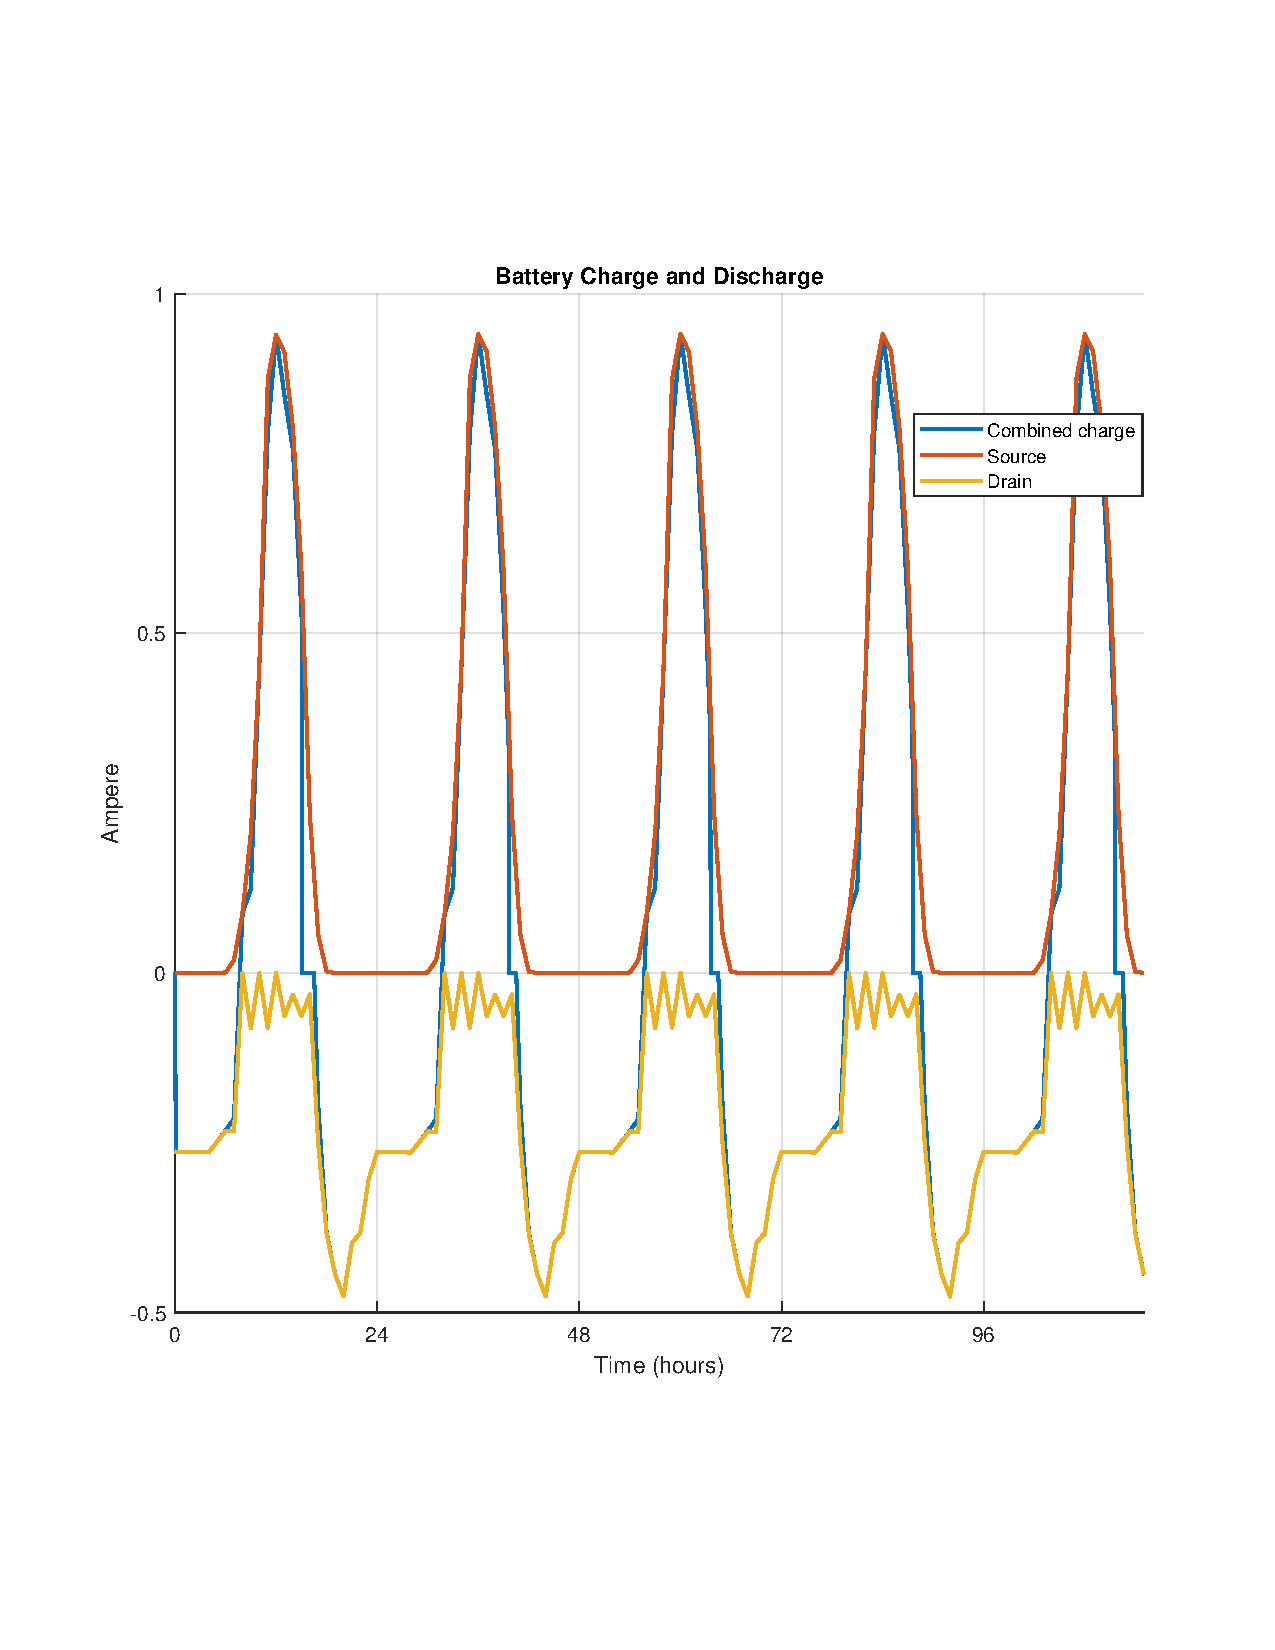
\includegraphics[width=\linewidth]{photos/Winter_charge_with_all_loss_5Days.pdf} %% Gjer denna om til kryss og sirkel
    \end{minipage}%
    \hspace{0.01\textwidth}% Adjust this to control the horizontal space between figure and table
    \begin{minipage}[t]{0.33\textwidth} % Adjust width so (width1 + hspace + width2) is about 1.0\textwidth
        \centering
        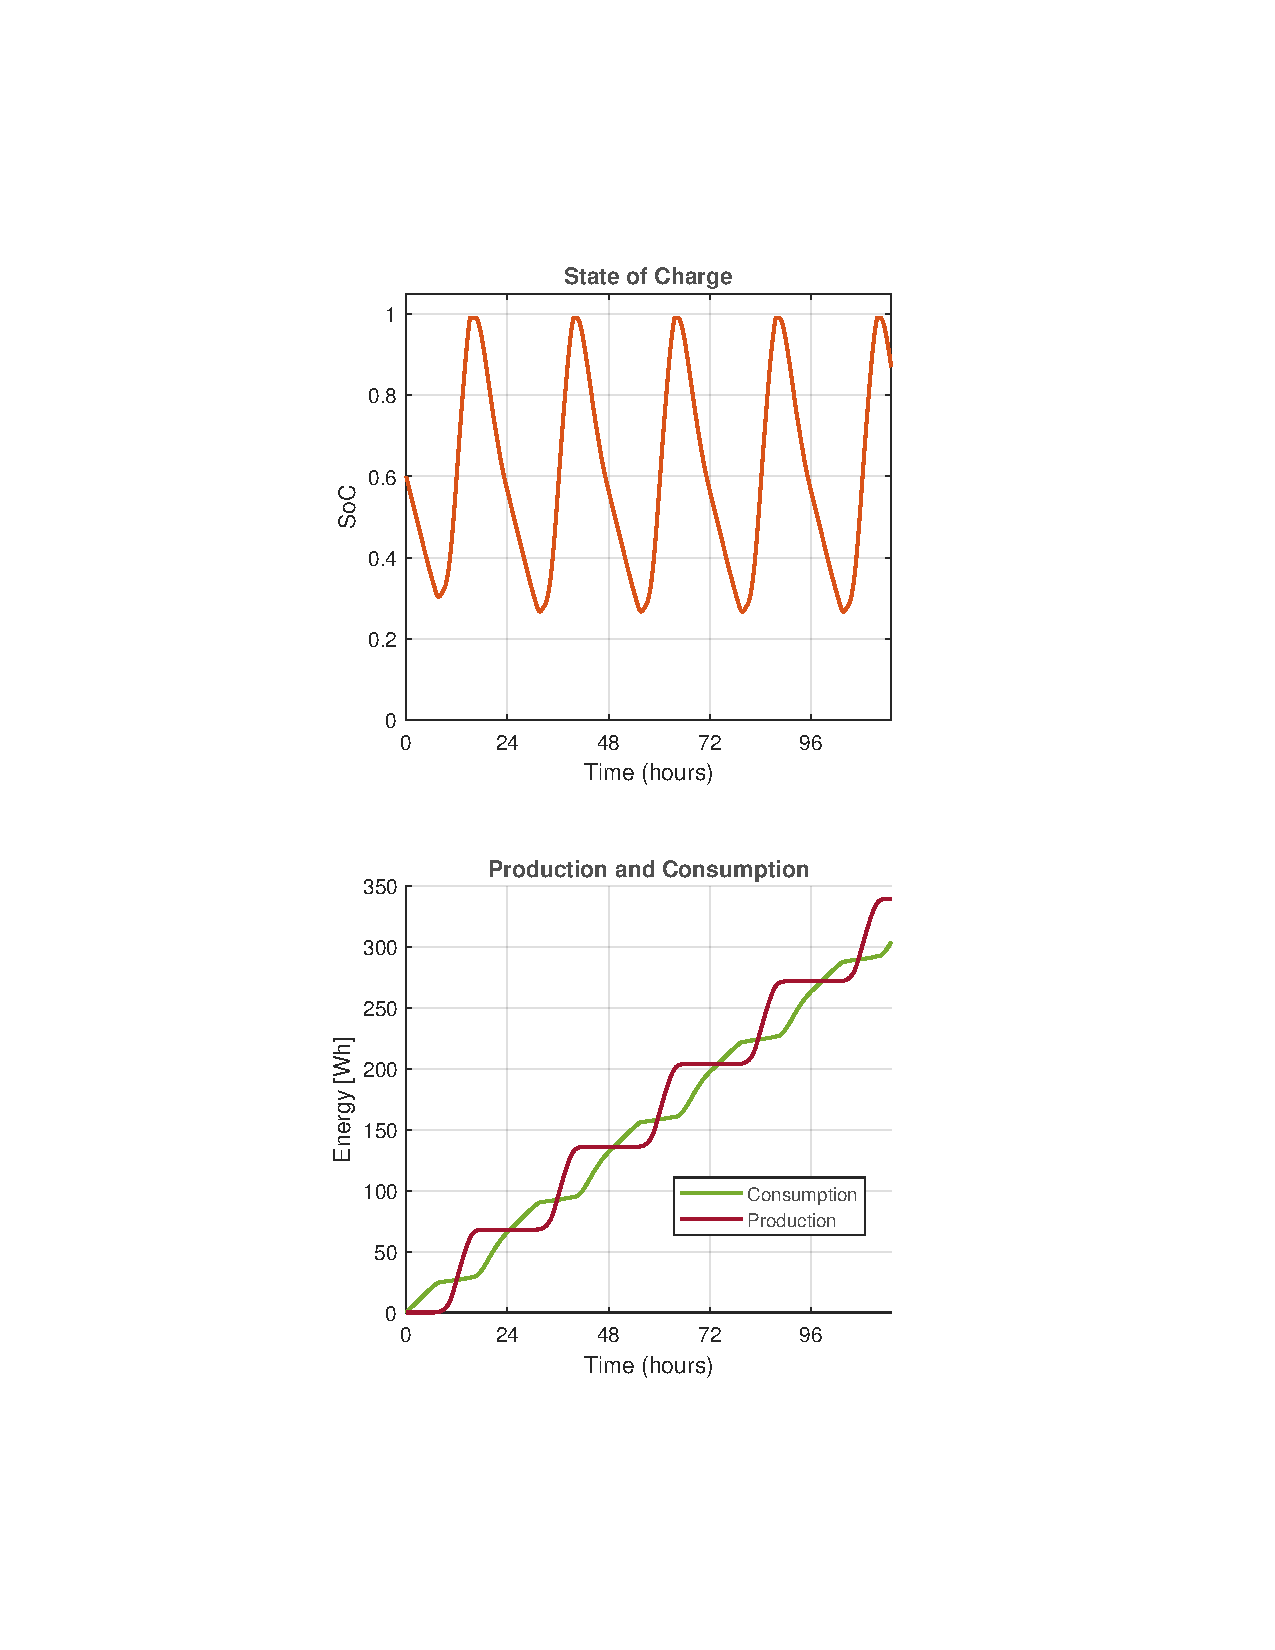
\includegraphics[width=\linewidth]{photos/Winter_SOC&Consumption_with_all_loss_5Days.pdf} %% Gjer denna om til kryss og sirkel
    \end{minipage}
    \captionsetup{font=footnotesize}
    \caption{Winter average production and consumption with all loss factors. Soiling 10\%, general transmission loss 14\% and effectiveness $\eta$ 79\%. The combined charge is the sum of production and consumption. State of charge is the battery charge. Power consumption is integrated from actual usage, and not production. Sample size of consumption profile is $n=19$.}
    \label{result:fig:Winter_40wpp_all_losses}
\end{figure}
The power consumption over five days is about \SI{300}{\watt\hour} of energy. As this cycle is barely stable, the consumption is almost equal to the production. We can see this from the consumption and production lines following each other closely. This gives a good utilization rate in terms of energy usage, using almost all the energy that it produces. 

Figure \ref{result:fig:Summer_40wpp_all_losses} shows a simulation with the summer data. With the increased irradiance in the summer months, this system charges to full each day. With lower consumption than winter, we also have a higher SoC throughout the 24-hour cycle. As seen from the combined charge, the battery stops charging at about peak hours.

\begin{figure}[H]
    \centering
    \begin{minipage}[t]{0.655\textwidth} % Adjust width as needed
        \centering
        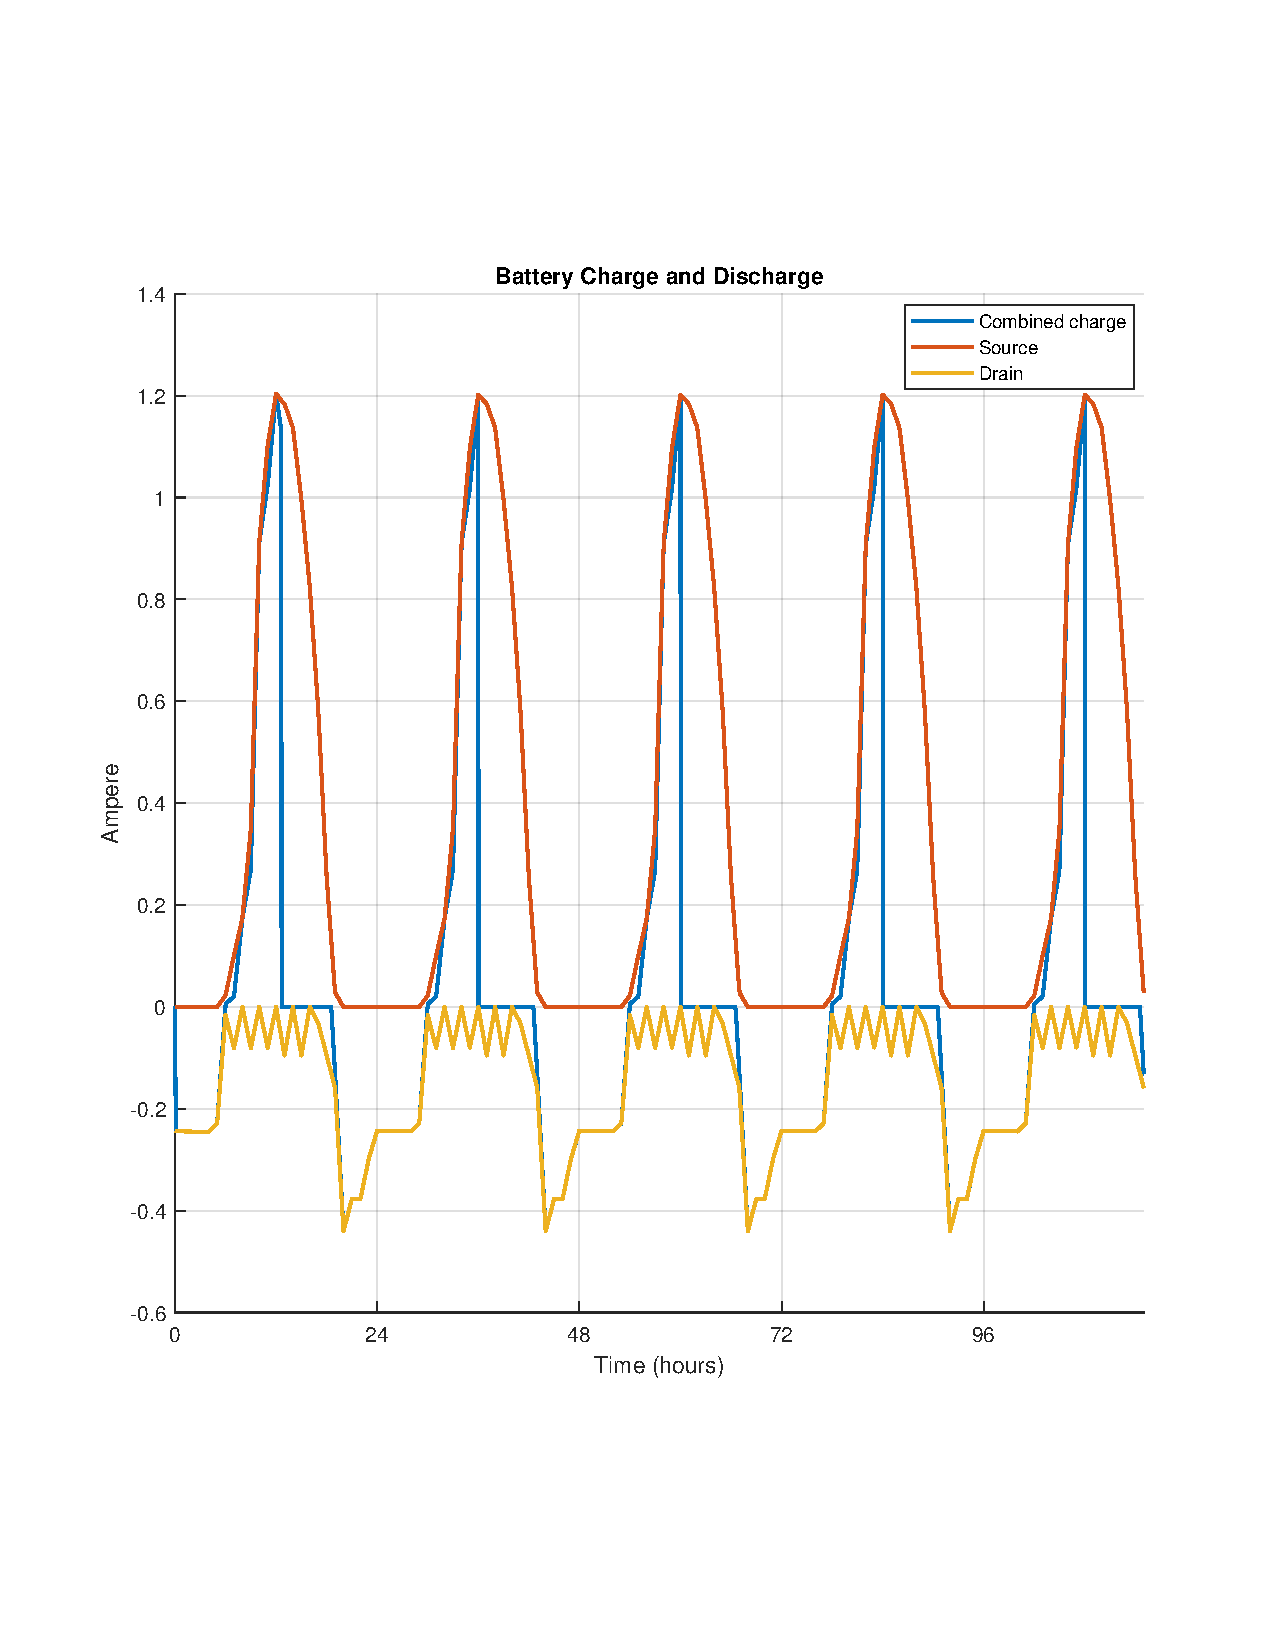
\includegraphics[width=\linewidth]{photos/Summer_charge_with_all_loss_5Days.pdf} %% Gjer denna om til kryss og sirkel
    \end{minipage}%
    \hspace{0.01\textwidth}% Adjust this to control the horizontal space between figure and table
    \begin{minipage}[t]{0.33\textwidth} % Adjust width so (width1 + hspace + width2) is about 1.0\textwidth
        \centering
        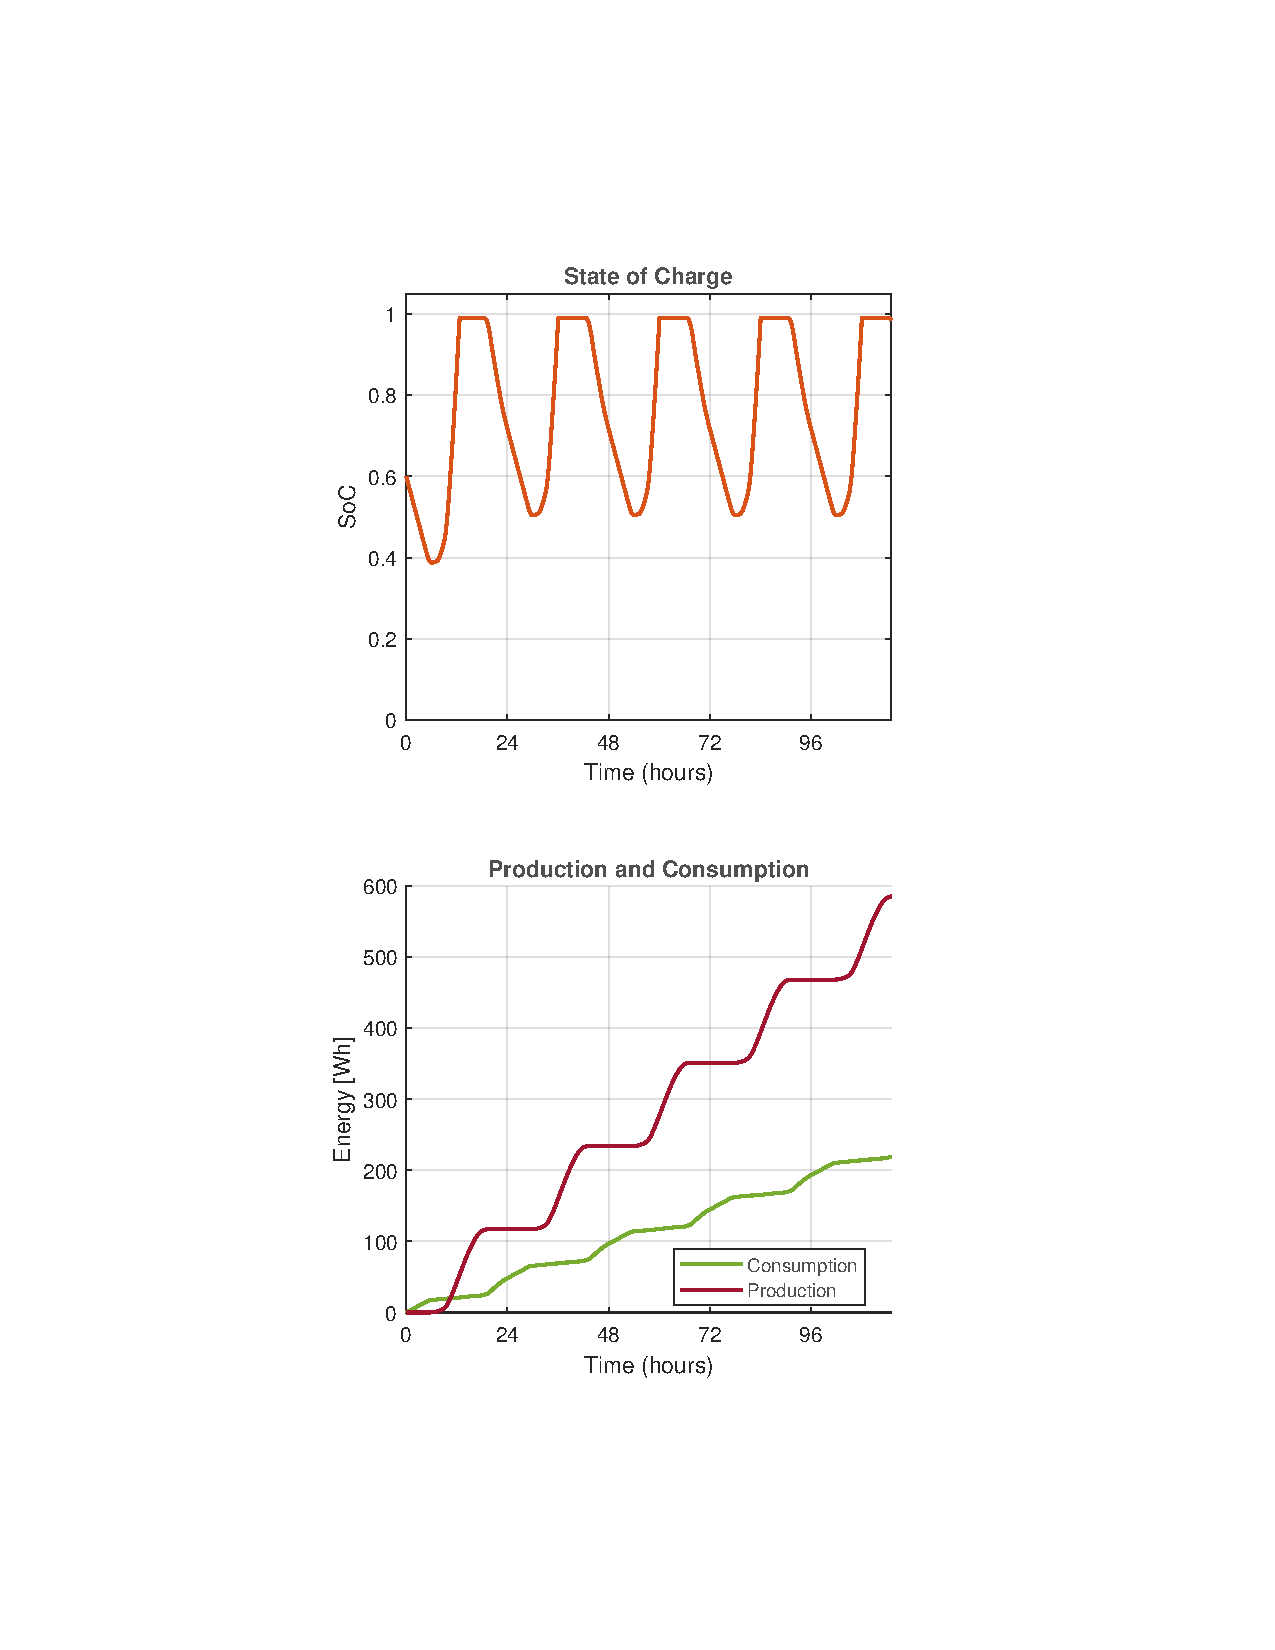
\includegraphics[width=\linewidth]{photos/Summer_SOC&Consumption_with_all_loss_5Days.pdf} %% Gjer denna om til kryss og sirkel
    \end{minipage}
    \captionsetup{font=footnotesize}
    \caption{Summer average production and consumption with all loss factors. Soiling 10\%, general transmission loss 14\% and effectiveness $\eta$ 79\%. The combined charge is the sum of production and consumption. State of charge is the battery charge. Power consumption is integrated from actual usage, and not production. Sample size of consumption profile is $n=19$.}
    \label{result:fig:Summer_40wpp_all_losses}
\end{figure}
Summer production outgrows the consumption, and although we produce almost \SI{600}{\watt\hour} - only about \SI{200}{\watt\hour} is consumed. This gives summer a lower utilization rate than winter. 
\newpage
\subsection{System specific simulations with daily load profile}
\label{sec:systemspesificdata}
\subsubsection{Summer data}
Figures \ref{result:fig:300_summer_soc}, \ref{result:fig:600_summer_soc} and \ref{result:fig:800_summer_soc} show the systems when compared towards the system specific consumption data. All loss factors are included. When using this setup, we risk having a small sample size for the consumption profile. 
\begin{minipage}[t]{0.32\textwidth} % Adjust width as needed
    \begin{figure}[H]
        \centering
        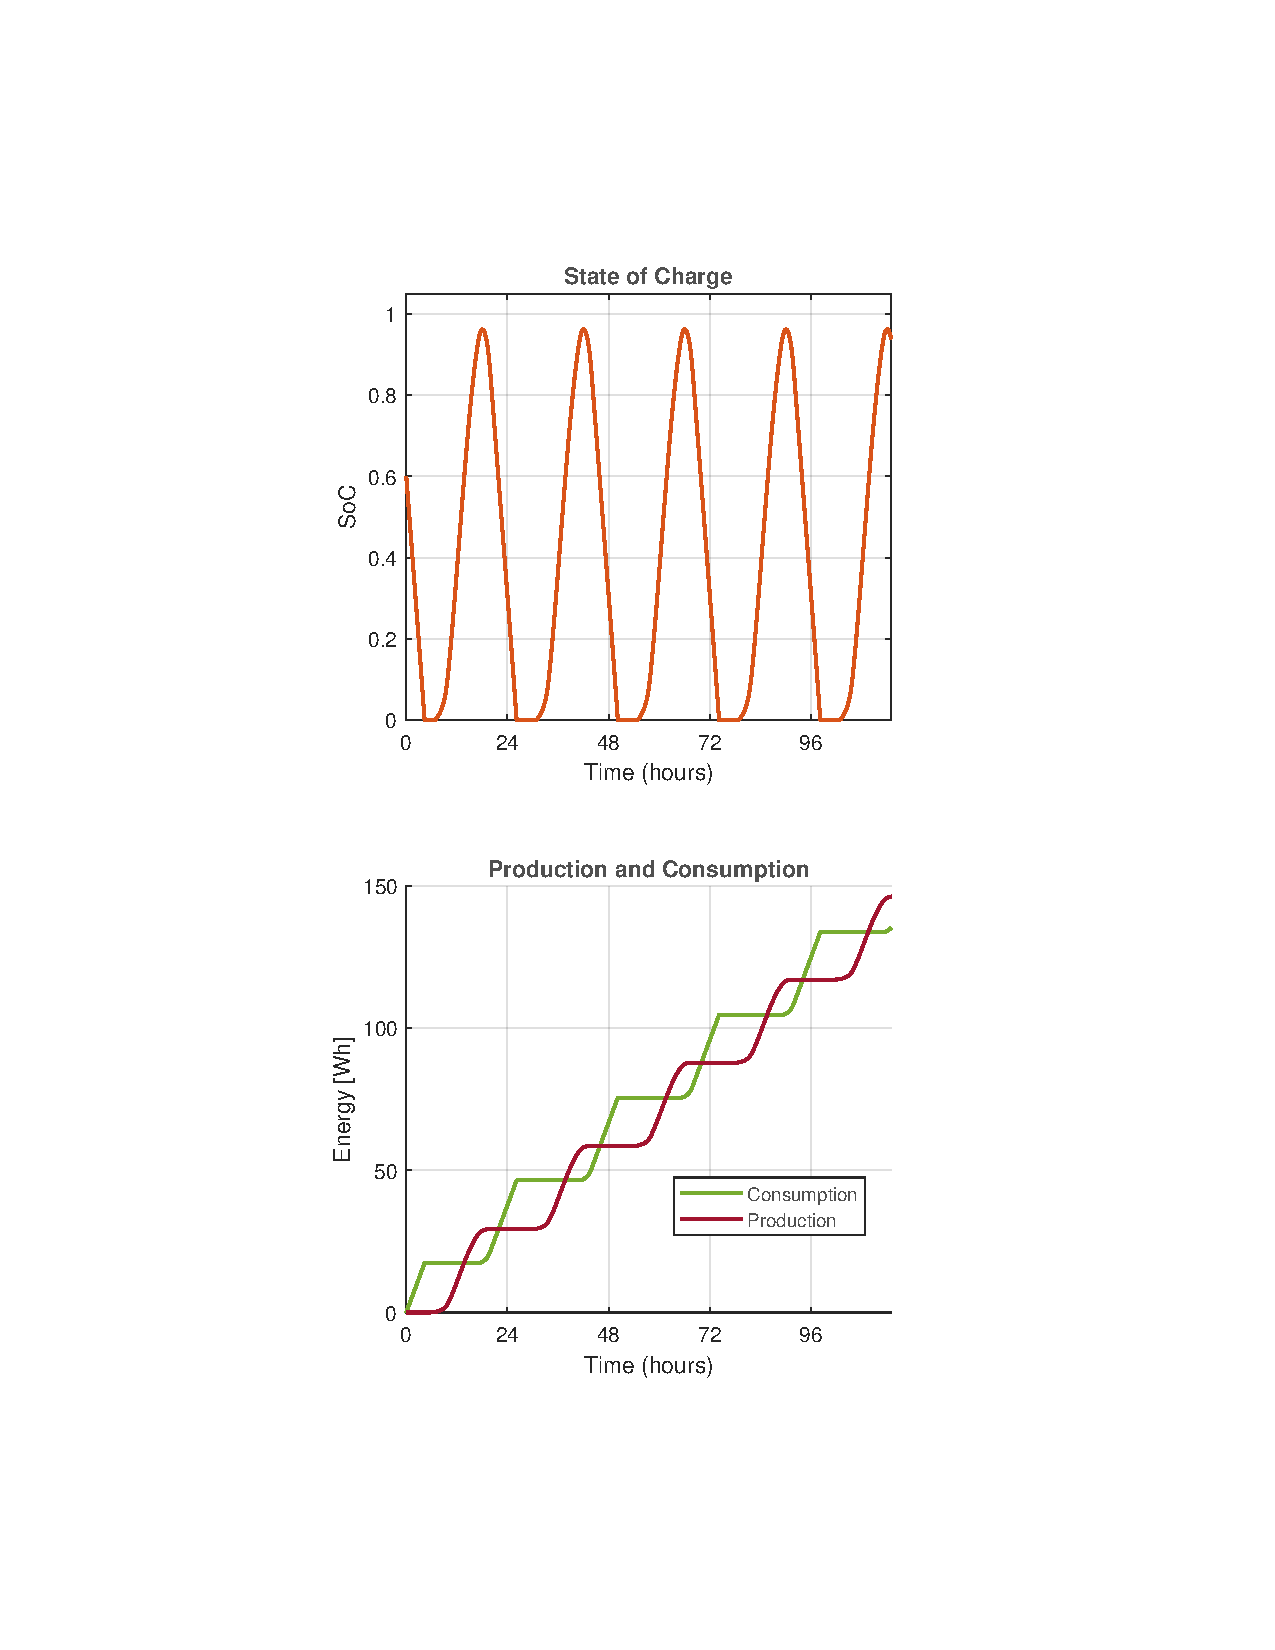
\includegraphics[width=\linewidth]{photos/Summer_SOC&Consumption_with_all_loss_5Days_300System.pdf} %% Gjer denna om til kryss og sirkel
        \captionsetup{font=footnotesize} % Or footnotesize, etc
        \caption{BH 300 System SoC, production and consumption for summer data. Soiling 10\%, general transmission loss 14\% and effectiveness $\eta$ 79\%.}
        \label{result:fig:300_summer_soc}
    \end{figure}
\end{minipage}% <--- IMPORTANT: The '%' symbol prevents unwanted horizontal space
\hspace{0.02\textwidth}% Adjust this to control the horizontal space between figure and table
\begin{minipage}[t]{0.32\textwidth} % Adjust width so (width1 + hspace + width2) is about 1.0\textwidth
    \begin{figure}[H]
        \centering
        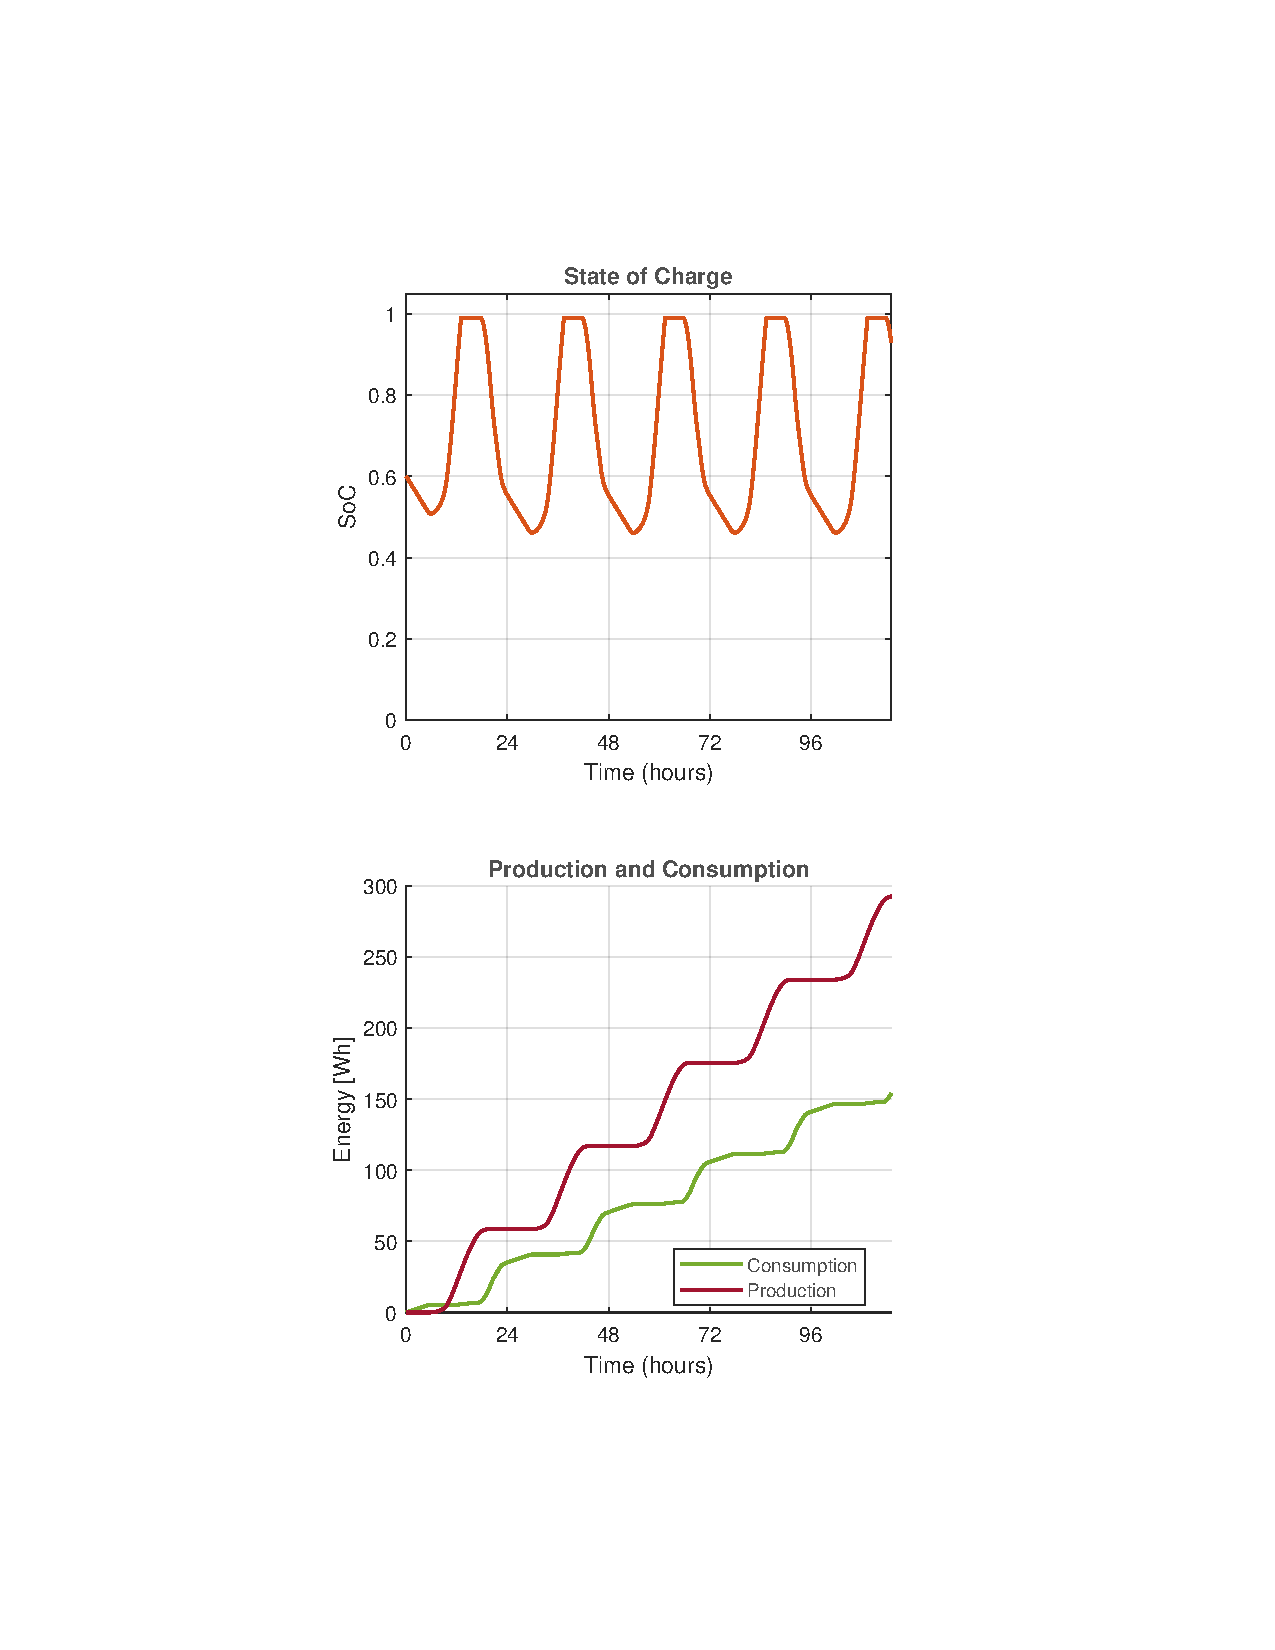
\includegraphics[width=\linewidth]{photos/Summer_SOC&Consumption_with_all_loss_5Days_600System.pdf} %% Gjer denna om til kryss og sirkel
        \captionsetup{font=footnotesize} % Or footnotesize, etc
        \caption{BH 600 System SoC, production and consumption for summer data. Soiling 10\%, general transmission loss 14\% and effectiveness $\eta$ 79\%.}
        \label{result:fig:600_summer_soc}
    \end{figure}
\end{minipage}
\hspace{0.02\textwidth}% Adjust this to control the horizontal space between figure and table
\begin{minipage}[t]{0.32\textwidth} % Adjust width so (width1 + hspace + width2) is about 1.0\textwidth
    \begin{figure}[H]
        \centering
        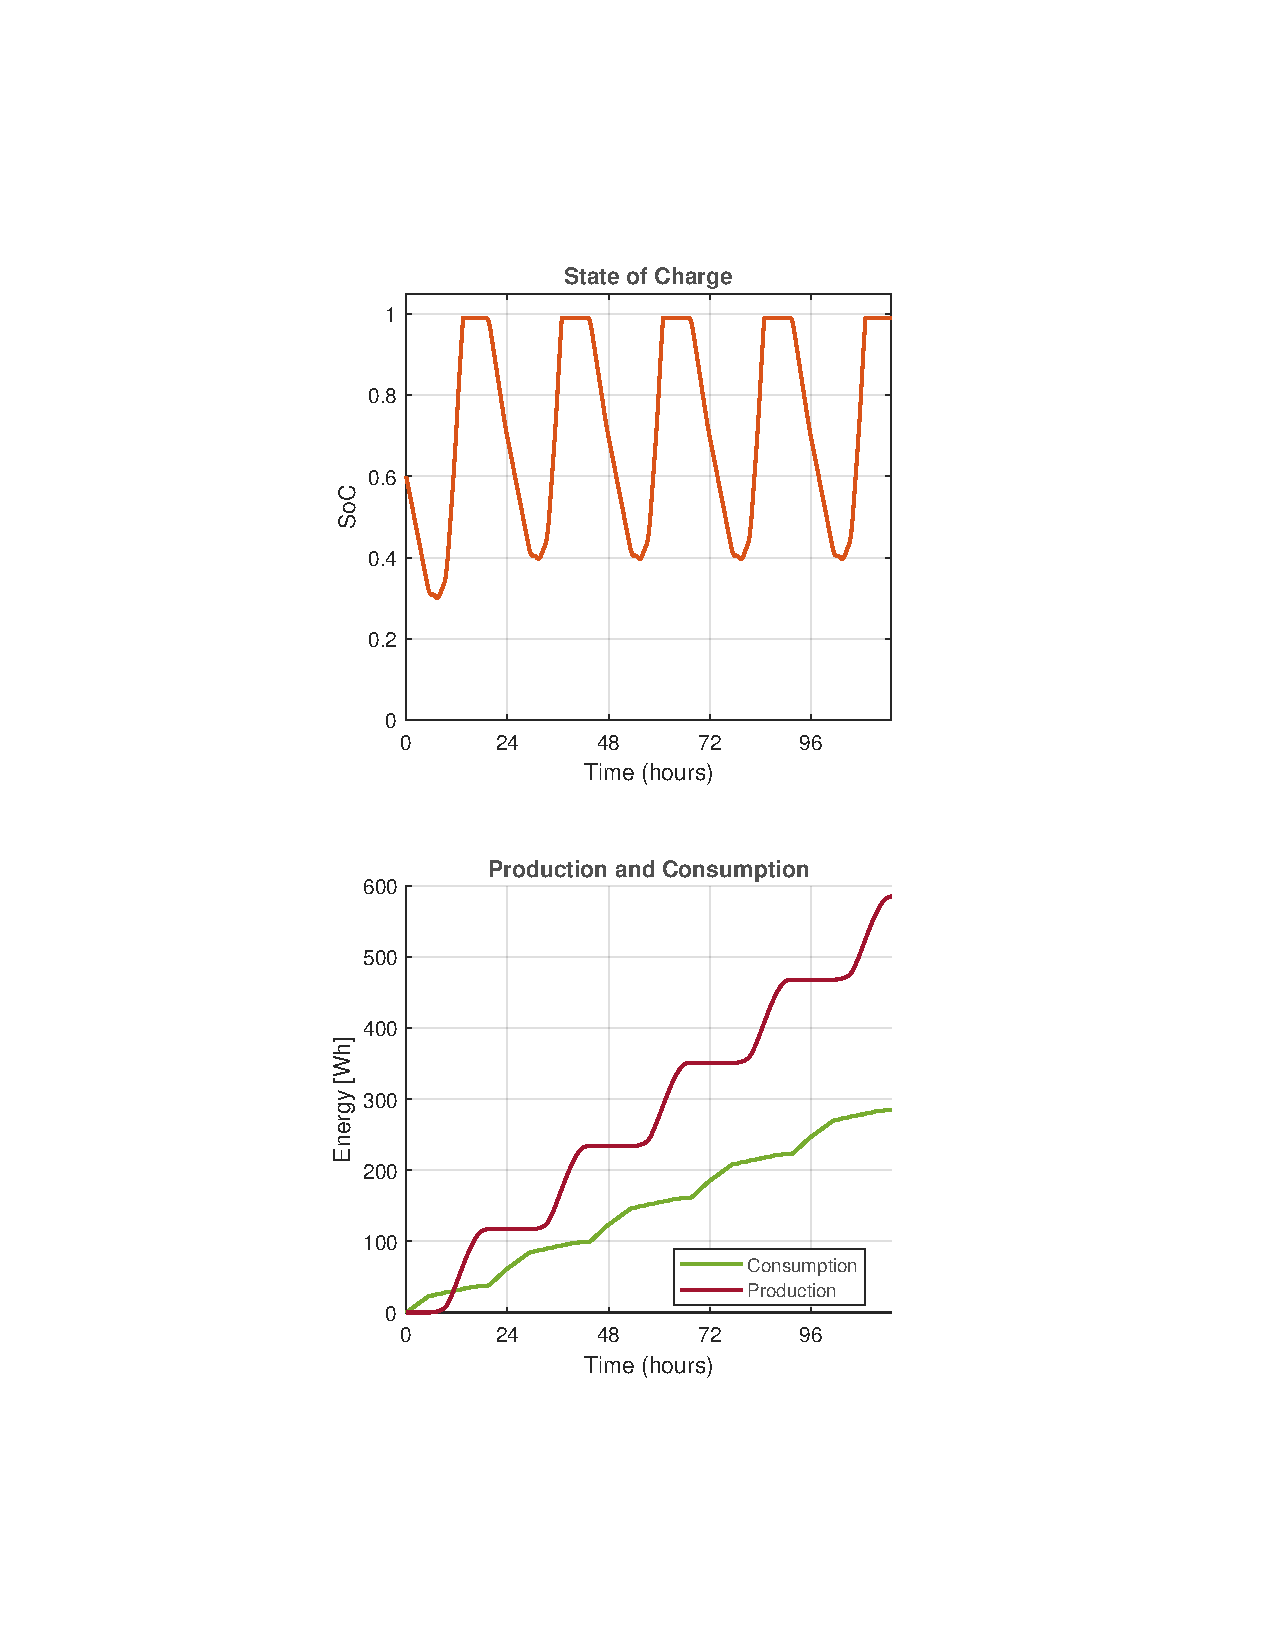
\includegraphics[width=\linewidth]{photos/Summer_SOC&Consumption_with_all_loss_5Days_800System.pdf} %% Gjer denna om til kryss og sirkel
        \captionsetup{font=footnotesize} % Or footnotesize, etc.
        \caption{BH 800 System SoC, production and consumption for summer data. Soiling 10\%, general transmission loss 14\% and effectiveness $\eta$ 79\%.}
        \label{result:fig:800_summer_soc}
    \end{figure}
\end{minipage}

Firstly we can see the difference in the consumption from the systems. BH 300 will consume at 140Wh, BH 600 will consume 150Wh, and BH 800 will consume 300Wh. We can also see the difference in the SoC, where the BH 300 will completely empty itself and almost receive a full charge in one day. For difference, the BH 600 and BH 800 will only use about half of their battery capacity. As this is during the summer months, we can assume a grater amplitude in the winter months. 
\newpage
\subsubsection{Winter data}
On figures \ref{result:fig:300_winter_soc}, \ref{result:fig:600_winter_soc} and \ref{result:fig:800_winter_soc} we can see the winter results with the same setup as the summer data. All loss factors are included.
\begin{minipage}[t]{0.32\textwidth} % Adjust width as needed
    \begin{figure}[H]
        \centering
        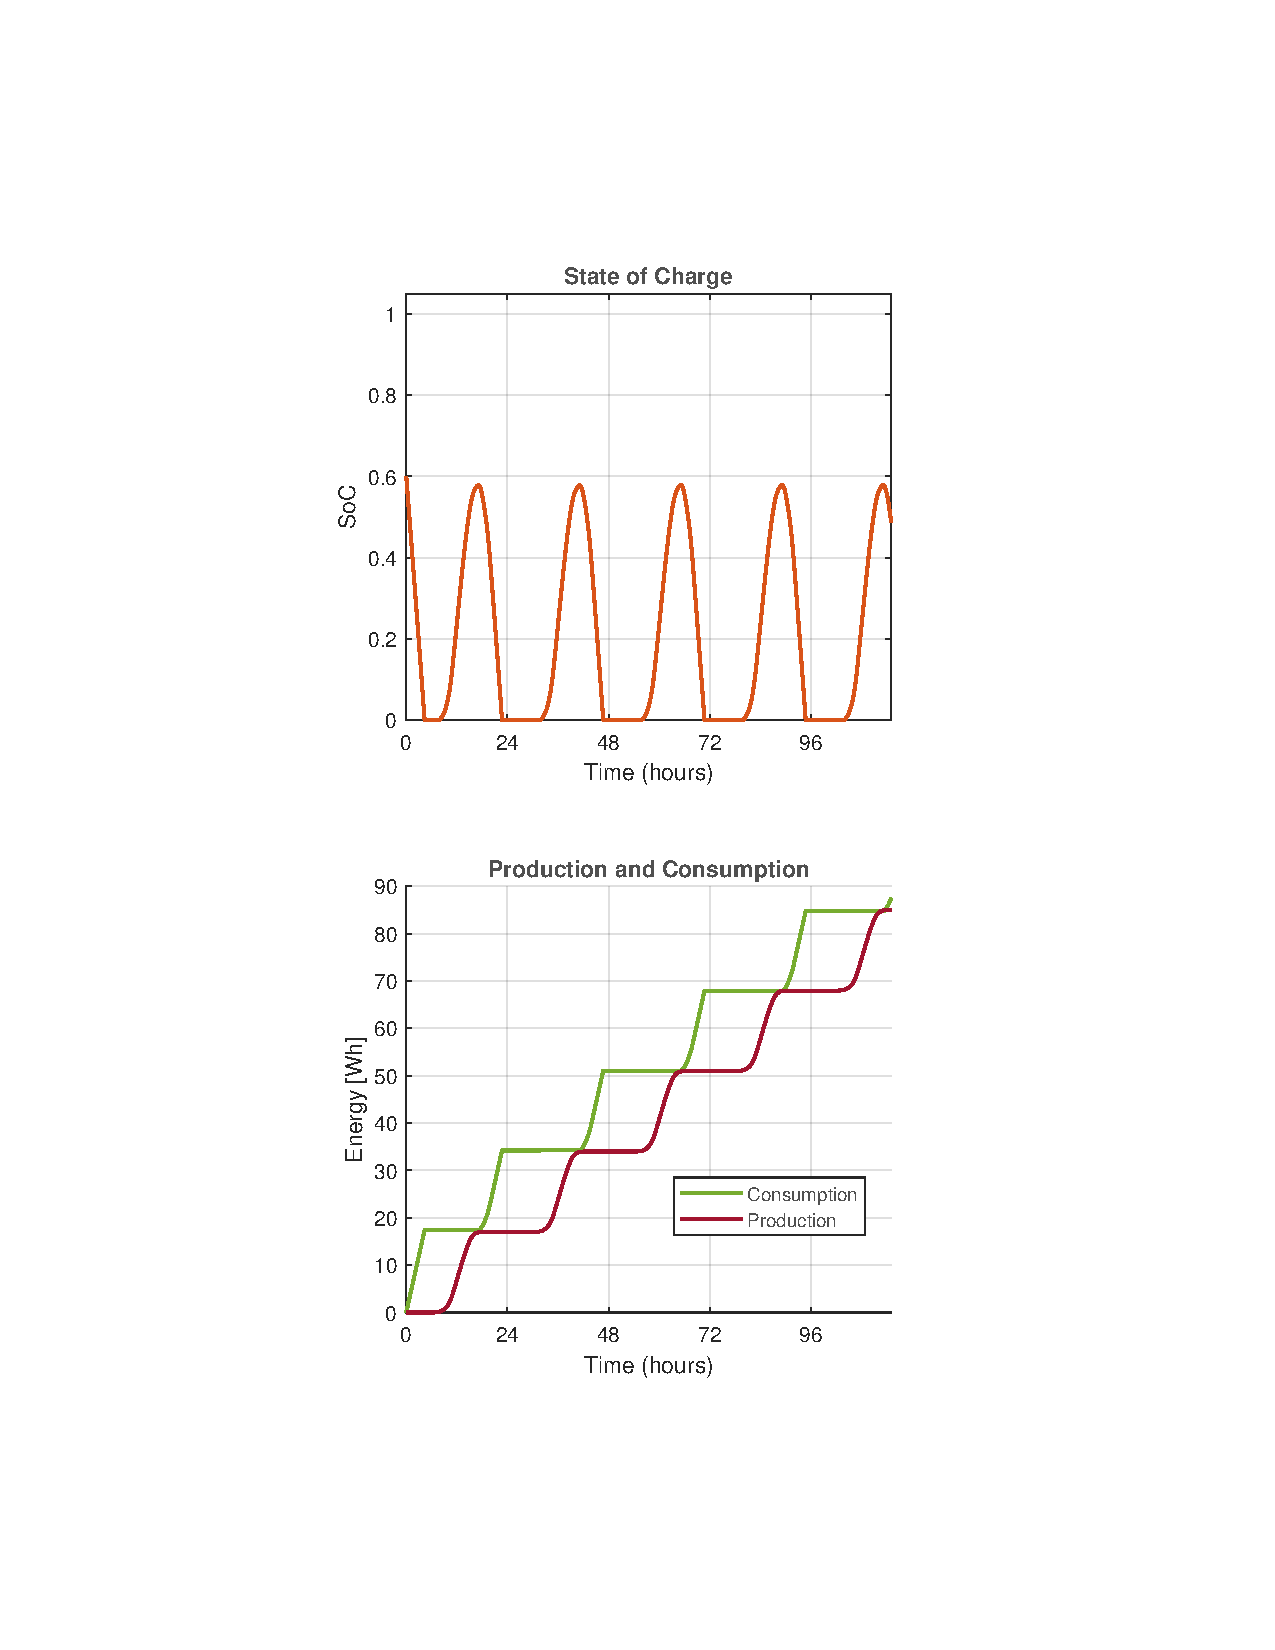
\includegraphics[width=\linewidth]{photos/Winter_SOC&Consumption_with_all_loss_5Days_300System.pdf} %% Gjer denna om til kryss og sirkel
        \captionsetup{font=footnotesize} % Or footnotesize, etc
        \caption{BH 300 System SoC, production and consumption for winter data. Soiling 10\%, general transmission loss 14\% and effectiveness $\eta$ 79\%.}
        \label{result:fig:300_winter_soc}
    \end{figure}
\end{minipage}% <--- IMPORTANT: The '%' symbol prevents unwanted horizontal space
\hspace{0.02\textwidth}% Adjust this to control the horizontal space between figure and table
\begin{minipage}[t]{0.32\textwidth} % Adjust width so (width1 + hspace + width2) is about 1.0\textwidth
    \begin{figure}[H]
        \centering
        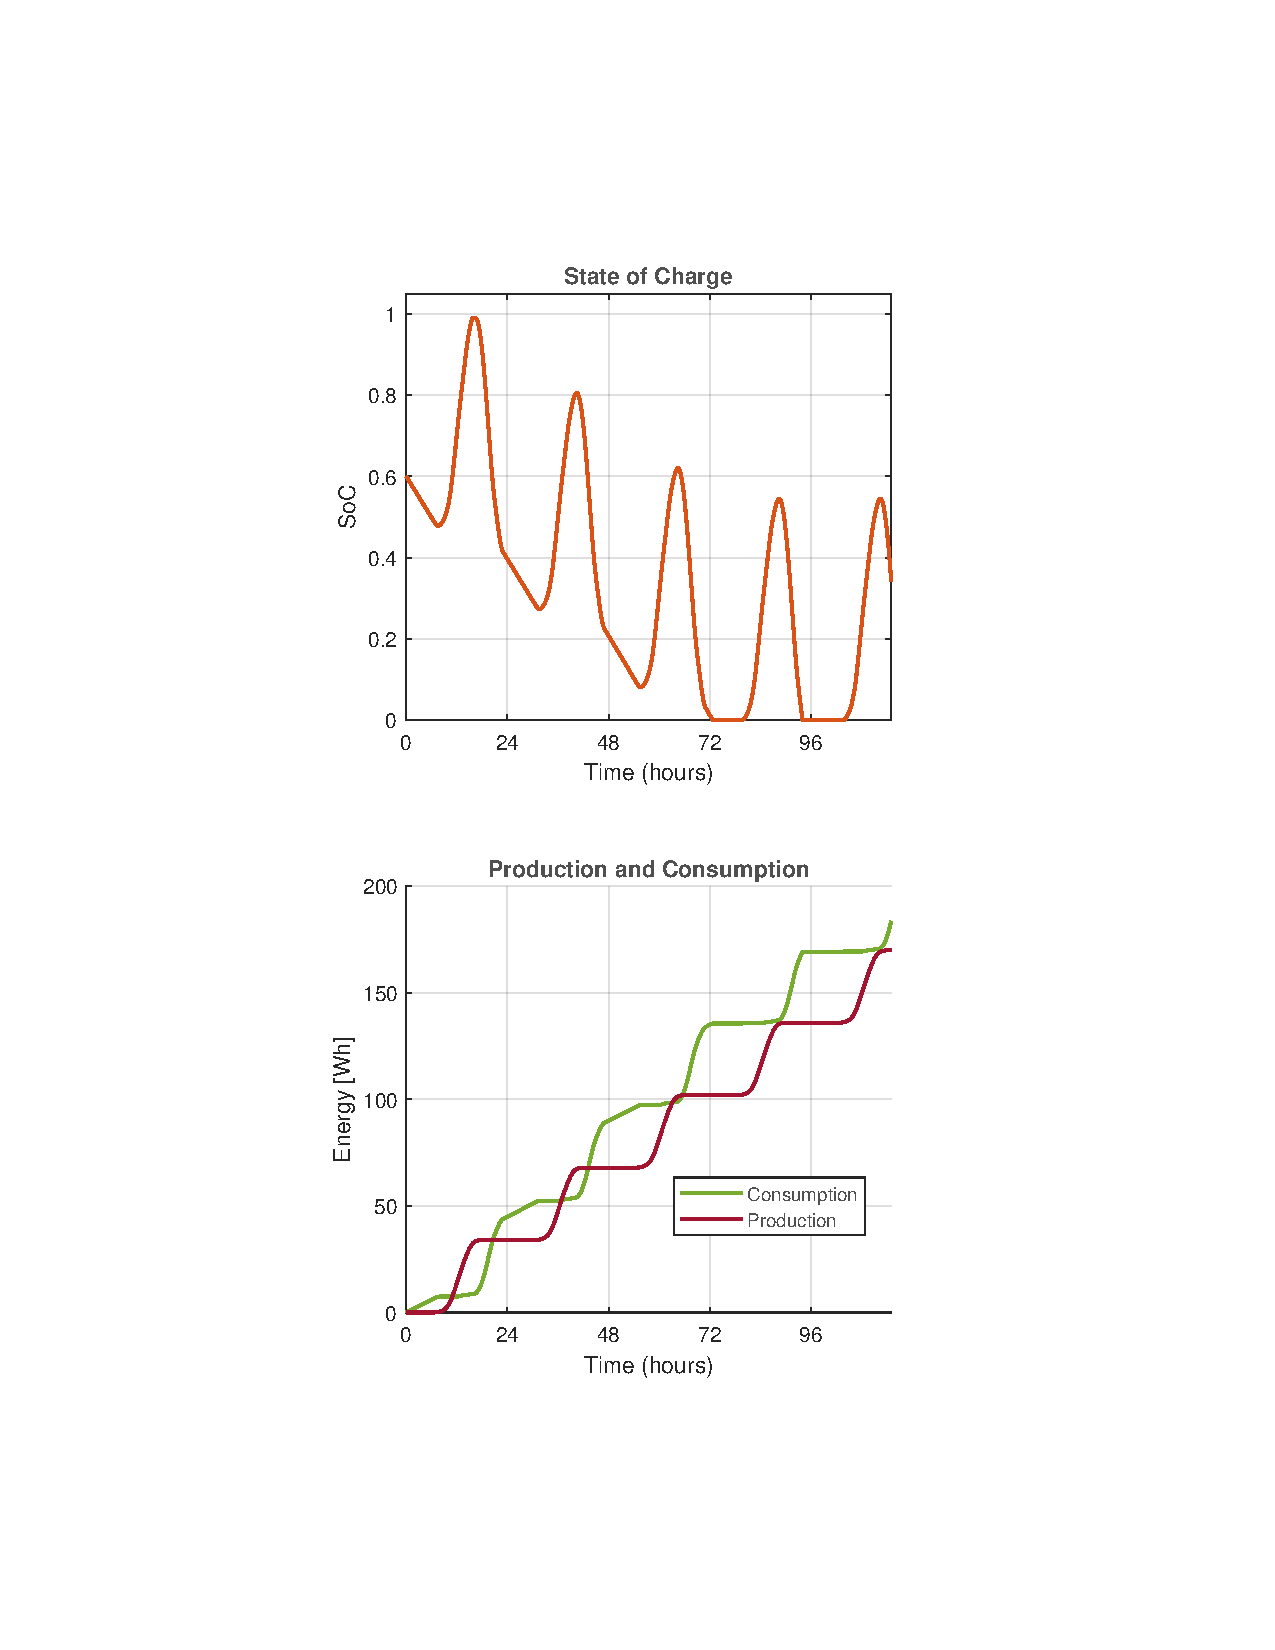
\includegraphics[width=\linewidth]{photos/Winter_SOC&Consumption_with_all_loss_5Days_600System.pdf} %% Gjer denna om til kryss og sirkel
        \captionsetup{font=footnotesize} % Or footnotesize, etc
        \caption{BH 600 System SoC, production and consumption for winter data. Soiling 10\%, general transmission loss 14\% and effectiveness $\eta$ 79\%.}
        \label{result:fig:600_winter_soc}
    \end{figure}
\end{minipage}
\hspace{0.02\textwidth}% Adjust this to control the horizontal space between figure and table
\begin{minipage}[t]{0.32\textwidth} % Adjust width so (width1 + hspace + width2) is about 1.0\textwidth
    \begin{figure}[H]
        \centering
        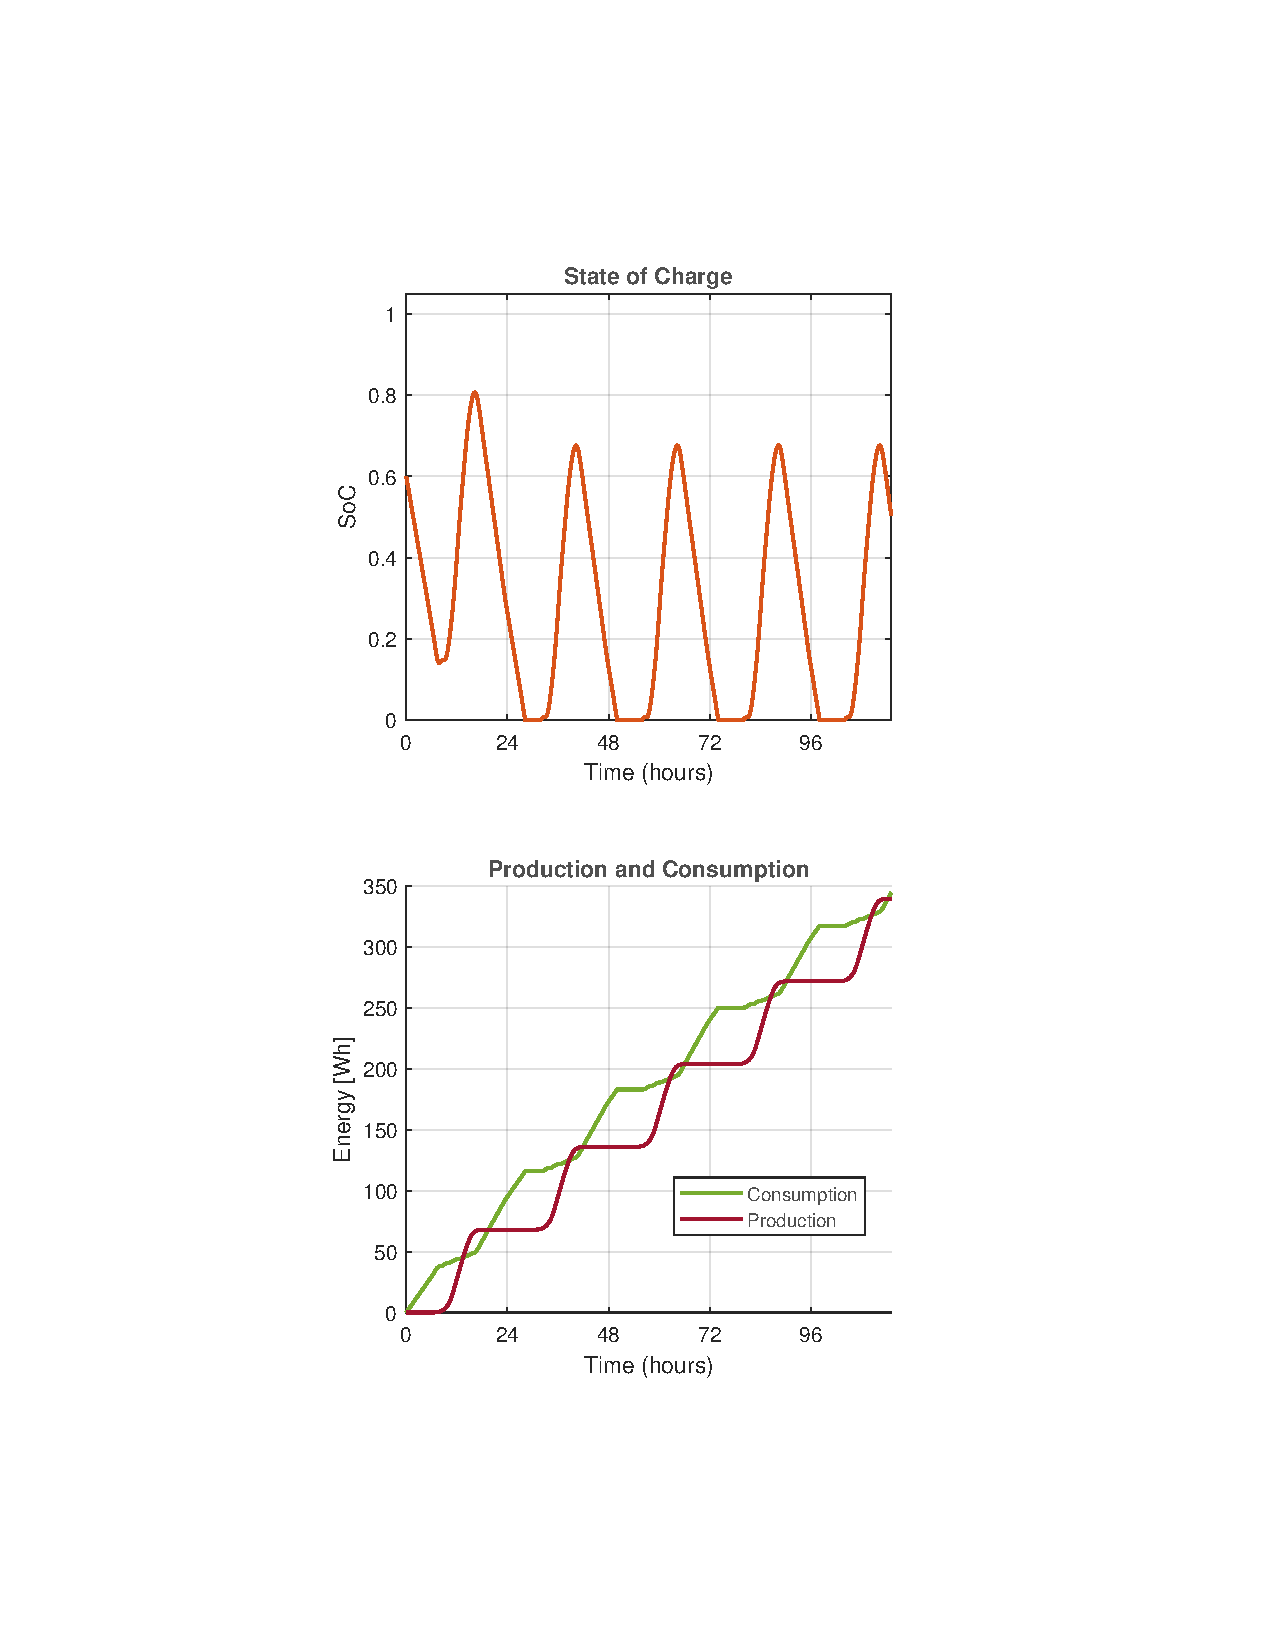
\includegraphics[width=\linewidth]{photos/Winter_SOC&Consumption_with_all_loss_5Days_800System.pdf} %% Gjer denna om til kryss og sirkel
        \captionsetup{font=footnotesize} % Or footnotesize, etc.
        \caption{BH 800 System SoC, production and consumption for winter data. Soiling 10\%, general transmission loss 14\% and effectiveness $\eta$ 79\%.}
        \label{result:fig:800_winter_soc}
    \end{figure}
\end{minipage}

Here we see all three of the systems hit an empty battery in under five days. All systems have full utilization rate based on their consumption. From the question: \textit{Does the battery ever run out, and what does it take to happen?}, the average answer was 2.5 times per year. Using this data, we can assume that the consumption changes according to the production. When cloudy or rainy weather reduces the production, the user reduce their consumption accordingly. 

\newpage
\section{Economical analysis}
On table \ref{tab:energy_summary} we find the annual production and consumption of each of the systems, according to their system specific data from section \ref{sec:systemspesificdata}. Consumption will for some systems match the production, when the system uses all the energy it produces. System BH 300 consumes all of it's production in both winter and summer months, which matches what we see from the simulations. The other systems has some excess production in at least one season. 

\begin{table}[H]
    \centering
    \begin{tabularx}{\linewidth}{|C|S[table-format=5.0]|S[table-format=5.0]|S[table-format=5.0]|S[table-format=5.0]|S[table-format=5.0]|S[table-format=5.0]|}
    \hline
    \textbf{System Name} & \multicolumn{3}{C|}{\textbf{Production (Wh)}} & \multicolumn{3}{C|}{\textbf{Consumption (Wh)}} \\ \cline{2-7}
     & \textbf{Winter} & \textbf{Summer} & \textbf{Annual} & \textbf{Winter} & \textbf{Summer} & \textbf{Annual} \\ \hline
    BH 800 (40Wpp) & 12147 & 21048 & \cellcolor{lightgray}33195 & 8445 & 7759 & \cellcolor{lightgray}16204 \\ \hline
    BH 600 (20Wpp) & 6073 & 10524 & \cellcolor{lightgray}16598 & 6073 & 6466 & \cellcolor{lightgray}12539 \\ \hline
    BH 300 (10Wpp) & 3037 & 5262 & \cellcolor{lightgray}8299 & 3037 & 5262 & \cellcolor{lightgray}8299 \\ \hline
    \end{tabularx}
    \caption{Yearly energy yield for each system based on total production and actual consumption. Sectioned into summer and winter months.}
    \label{tab:energy_summary}
\end{table}
With this data, we can analyze the LCOE and Payback time. Doing an annual calculation for both of these metrics is the most common, and with the data from the table we can do an individual evaluation of all the systems. 

\subsection{LCOE}
In tables \ref{tab:lcoe_qty_prod_5_condensed} and \ref{tab:lcoe_qty_cons_5_condensed} we find the LCOE for the systems with a 5\% discount rate. In tables \ref{tab:lcoe_qty_prod_75_condensed} and \ref{tab:lcoe_qty_cons_75_condensed}, we find for 7.5\%. Lastly the LCOE without discount is shown in table \ref{tab:lcoe_qty_prod_no_discount_condensed}, to compare against similar projects that don't use discount rate. The basis for lifetime is from section \ref{chap:method:sec:LCOE}, but is rounded to whole years. Costs are gathered from table \ref{table:SHS_cost}, where only the quantity price is used. The calculation of LCOE is based on equation \eqref{eq:LCOEfirst}. 

The tables take into account two sets of energy data, both the produced and the consumed. This will compare the potential of the system towards the cost, as well as the actual usage of the system towards the cost. There is also a leap in the lifetime that is shown. Systems are designed for a lifetime of 6-7 years, and at least 2000 cycles. As explained in section \ref{chap:method:sec:LCOE} this is can be under 6 years, which is why 5 years is added. 25 years is 9000 cycles, which was also found in section \ref{chap:method:sec:LCOE} to be the maximum for a battery. 
\small % Apply to the entire set of tables for better fitting

%\noindent % Ensure no paragraph indentation before the minipages
\begin{minipage}[t]{0.45\textwidth}
\centering % Center content within this minipage

% --- Tables for 5% Discount Rate (Left Column) ---

% Table 1: Quantity Price from Production (5% Discount)
\begin{table}[H]
\centering
\begin{tabularx}{\linewidth}{|>{\RaggedRight\hsize=0.25\hsize}X|>{\Centering\hsize=0.25\hsize}X|>{\Centering\hsize=0.25\hsize}X|>{\Centering\hsize=0.25\hsize}X|}
\hline
 \textbf{Lifetime}& \textbf{BH 300} & \textbf{BH 600} & \textbf{BH 800} \\
\hline
\textbf{$L_{5}$} & 28.8 & 18.6 & 12.9 \\ \hline
\textbf{$L_{6}$} & 24.5 & 15.8 & 11.0 \\ \hline
\textbf{$L_{7}$} & 21.5 & 13.9 & 9.6 \\ \hline
\textbf{$L_{8}$} & 19.3 & 12.4 & 8.6 \\ \hline
\textbf{$L_{25}$} & 8.8 & 5.7 & 4.0 \\ \hline
\end{tabularx}
\caption{LCOE for total production with $r=0.05$. Values in EUR/kWh.}
\label{tab:lcoe_qty_prod_5_condensed}
\end{table}

% Table 2: Quantity Price from Consumption (5% Discount)
\begin{table}[H]
\centering
\begin{tabularx}{\linewidth}{|>{\RaggedRight\hsize=0.25\hsize}X|>{\Centering\hsize=0.25\hsize}X|>{\Centering\hsize=0.25\hsize}X|>{\Centering\hsize=0.25\hsize}X|}
\hline
 \textbf{Lifetime}& \textbf{BH 300} & \textbf{BH 600} & \textbf{BH 800} \\
\hline
\textbf{$L_{5}$} & 28.8 & 24.6 & 26.4 \\ \hline
\textbf{$L_{6}$} & 24.5 & 20.9 & 22.5 \\ \hline
\textbf{$L_{7}$} & 21.5 & 18.4 & 19.7 \\ \hline
\textbf{$L_{8}$} & 19.3 & 16.5 & 17.7 \\ \hline
\textbf{$L_{25}$} & 8.8 & 7.5 & 8.1 \\ \hline
\end{tabularx}
\caption{LCOE for actual consumption with $r=0.05$. Values in EUR/kWh.}
\label{tab:lcoe_qty_cons_5_condensed}
\end{table}

\end{minipage}\hfill % Separator between left and right columns
\begin{minipage}[t]{0.45\textwidth}
\centering % Center content within this minipage

% --- Tables for 7.5% Discount Rate (Right Column) ---

% Table 3: Quantity Price from Production (7.5% Discount)
\begin{table}[H]
\centering
\begin{tabularx}{\linewidth}{|>{\RaggedRight\hsize=0.25\hsize}X|>{\Centering\hsize=0.25\hsize}X|>{\Centering\hsize=0.25\hsize}X|>{\Centering\hsize=0.25\hsize}X|}
\hline
 \textbf{Lifetime}& \textbf{BH 300} & \textbf{BH 600} & \textbf{BH 800} \\
\hline
\textbf{$L_{5}$} & 30.8 & 19.9 & 13.8 \\ \hline
\textbf{$L_{6}$} & 26.5 & 17.1 & 11.9 \\ \hline
\textbf{$L_{7}$} & 23.5 & 15.2 & 10.5 \\ \hline
\textbf{$L_{8}$} & 21.3 & 13.7 & 9.5 \\ \hline
\textbf{$L_{25}$} & 11.2 & 7.2 & 5.0 \\ \hline
\end{tabularx}
\caption{LCOE for total production with $r=0.075$. Values in EUR/kWh.}
\label{tab:lcoe_qty_prod_75_condensed}
\end{table}

% Table 4: Quantity Price from Consumption (7.5% Discount)
\begin{table}[H]
\centering
\begin{tabularx}{\linewidth}{|>{\RaggedRight\hsize=0.25\hsize}X|>{\Centering\hsize=0.25\hsize}X|>{\Centering\hsize=0.25\hsize}X|>{\Centering\hsize=0.25\hsize}X|}
\hline
 \textbf{Lifetime}& \textbf{BH 300} & \textbf{BH 600} & \textbf{BH 800} \\
\hline
\textbf{$L_{5}$} & 30.8 & 26.3 & 28.2 \\ \hline
\textbf{$L_{6}$} & 26.5 & 22.7 & 24.3 \\ \hline
\textbf{$L_{7}$} & 23.5 & 20.1 & 21.6 \\ \hline
\textbf{$L_{8}$} & 21.3 & 18.2 & 19.5 \\ \hline
\textbf{$L_{25}$} & 11.2 & 9.5 & 10.2 \\ \hline
\end{tabularx}
\caption{LCOE for actual consumption with $r=0.075$. Values in EUR/kWh.}
\label{tab:lcoe_qty_cons_75_condensed}
\end{table}

\end{minipage}

\vspace{1em} % Add some vertical space before the next table, adjust as needed

% --- Table for No Discount Rate (Centered Below) ---
\begin{table}[H]
\centering
\begin{tabularx}{0.5\textwidth}{|>{\RaggedRight\hsize=0.25\hsize}X|>{\Centering\hsize=0.25\hsize}X|>{\Centering\hsize=0.25\hsize}X|>{\Centering\hsize=0.25\hsize}X|}
\hline
 \textbf{Lifetime}& \textbf{BH 300} & \textbf{BH 600} & \textbf{BH 800} \\
\hline
\textbf{$L_{5}$} & 24.9 & 16.1 & 11.1 \\ \hline
\textbf{$L_{6}$} & 20.8 & 13.4 & 9.3 \\ \hline
\textbf{$L_{7}$} & 17.8 & 11.5 & 8.0 \\ \hline
\textbf{$L_{8}$} & 15.6 & 10.0 & 7.0 \\ \hline
\textbf{$L_{25}$} & 5.0 & 3.2 & 2.2 \\ \hline
\end{tabularx}
\caption{LCOE without discount rate ($r=0$) from production. Values in EUR/kWh.}
\label{tab:lcoe_qty_prod_no_discount_condensed}
\end{table}

With a lifetime 8 or less years, the LCOE for a SHS is unprofitable at best. BH 800 fares best in the comparison for energy production, having a lower LCOE than BH 300 and BH 600. As the price of the system is not linear with the size of the panel, it benefits from a marginal increase in panel size compared to marginal price increase. When looking at the consumption data, the systems don't differ as much. BH 600 has the lowest LCOE, with BH 800 being in the middle and BH 300 being the highest. 

\subsection{Payback time}
To find the payback time we use quantity cost, energy consumption and electricity price. In addition, we add the fair price that the participants feel is justified for the system. Payback time is show in figure \ref{result:fig:paybacktime}.


\begin{minipage}[t]{0.65\textwidth} % Adjust width as needed
    \begin{figure}[H]
        \centering
        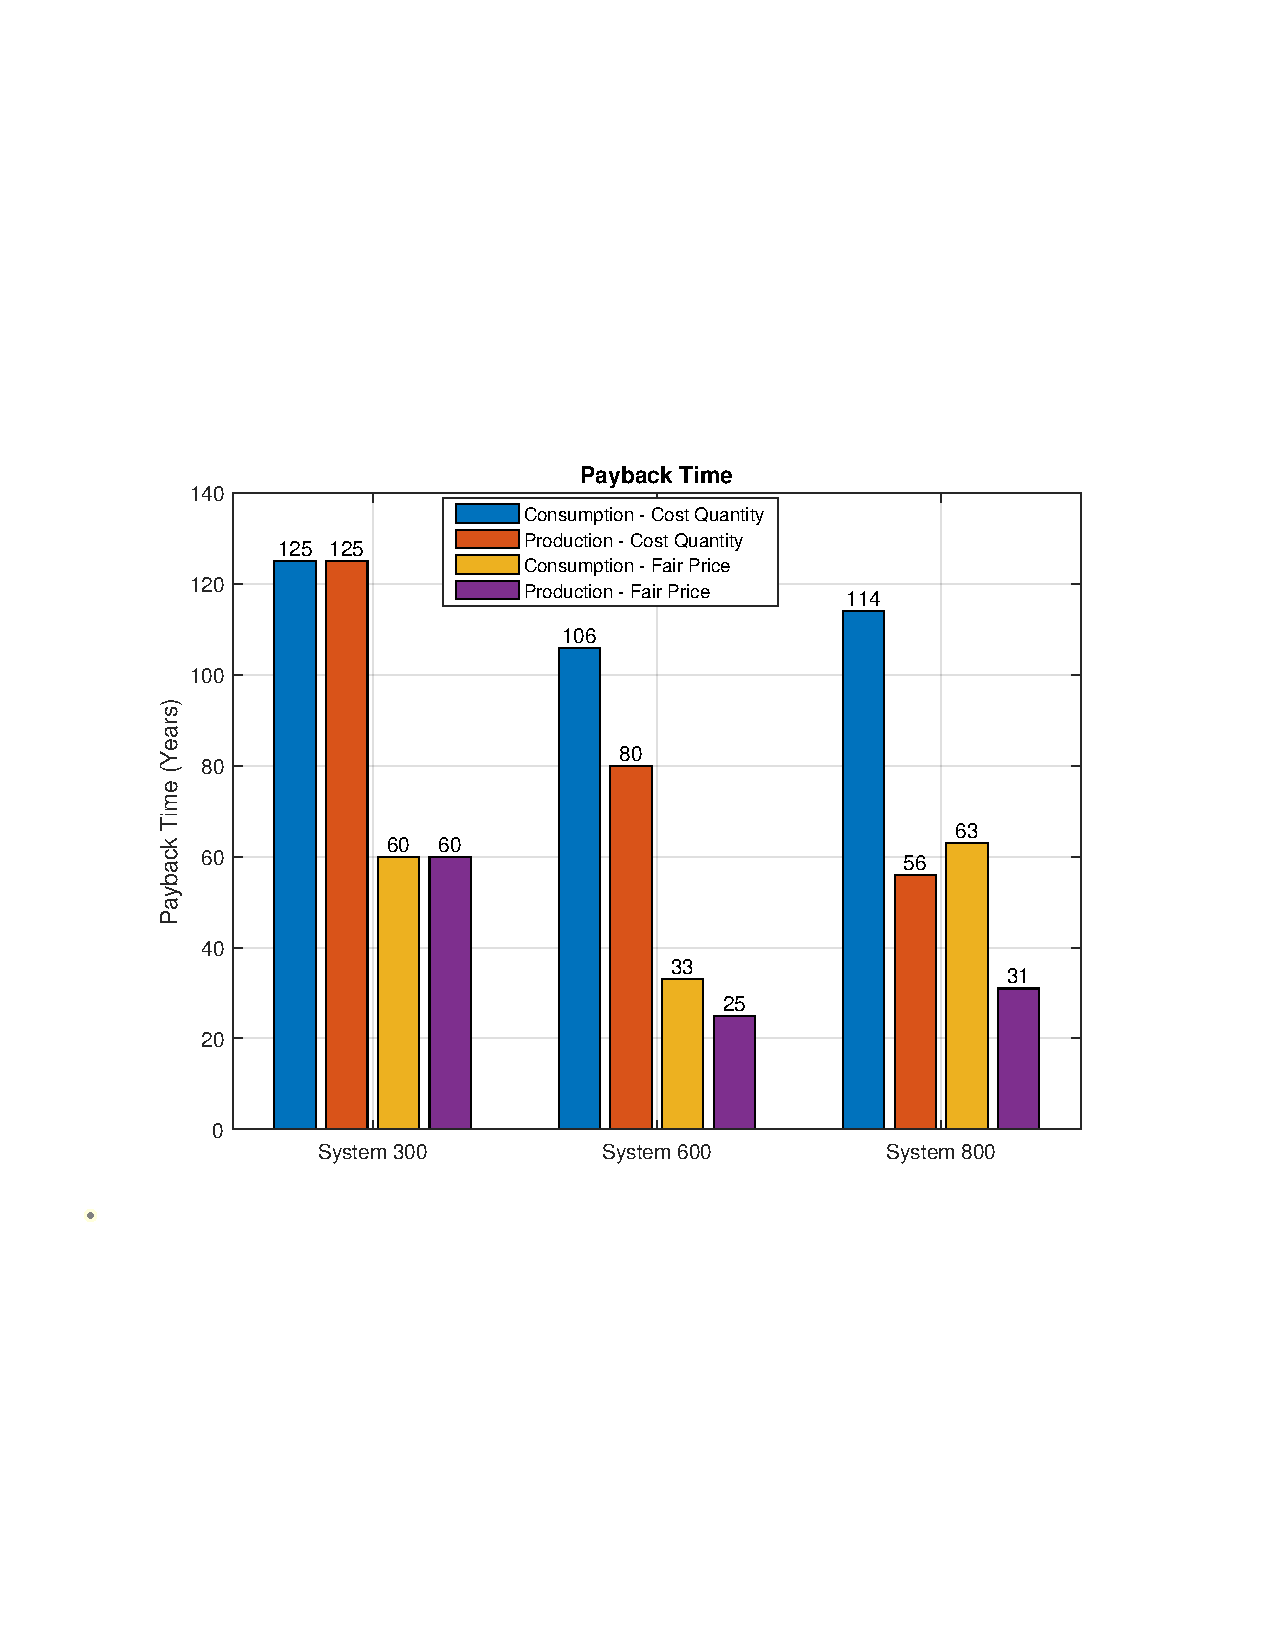
\includegraphics[width=\linewidth]{photos/PaybackTime_comparison_barChart.pdf} %% Gjer denna om til kryss og sirkel
        \captionsetup{font=small}
        \caption{Payback time using actual consumption and total production data from table \ref{tab:energy_summary}, with the electricity price from \ref{method:fig:EU27_elecprice}. Prices are shown in table \ref{tab:fair&quan_price} to the left of the figure.}
        \label{result:fig:paybacktime}
    \end{figure}
\end{minipage}% <--- IMPORTANT: The '%' symbol prevents unwanted horizontal space
%\vspace{0.1\textwidth}
\begin{minipage}[t]{0.35\textwidth}
    \vspace{0.25\textwidth}
    \begin{table}[H]
        \centering
        \small
        \begin{tabularx}{\linewidth}{|>{\RaggedRight\arraybackslash\hsize=0.30\hsize}X|>{\Centering\arraybackslash\hsize=0.30\hsize}X|>{\Centering\arraybackslash\hsize=0.30\hsize}X|}
        \hline
        \multicolumn{3}{|c|}{System prices} \\
        \hline
        System & Quantity price & Fair Price \\
        \hline
        BH 300 & 124 & 60\\ \hline
        BH 600 & 160 & 50  \\ \hline
        BH 800 & 222 & 123 \\ \hline
        \end{tabularx}
        \captionsetup{font=small}
        \caption{Quantity price is gathered from table \ref{table:SHS_cost}. Fair price was a question asked to participants in the interviews, see appendix \ref{apx:ftquestions}. Sample size for fair price is $n<3$, so the data is inaccurate.}
        \label{tab:fair&quan_price} 
    \end{table}
\end{minipage}

Economical payback time ranges from 125 years to 25 years, where 25 years is using the fair price from participants answers. With lifetime of 6-7 years, the economical benefits of the system will not cover the costs during a normal lifetime. Although the system might last longer, the benefits will likely never surpass the cost of the system. This is true regardless of which system we compare. 

\section{Social analysis}

\subsection{Energy sources}
To analyze how SHS has affected households, we wanted to take a look at their current energy sources. Household energy sources can be found on figure \ref{res:soc:householdenergysources}. Although Albania has full grid coverage, we looked at how many of the participants that actually were connected to the grid. Figure \ref{res:soc:gridconnection} shows the results of connection, off-grid and illegal connection.
\begin{figure}[H]
    \centering
    \begin{subfigure}[b]{0.48\textwidth}
        \centering
        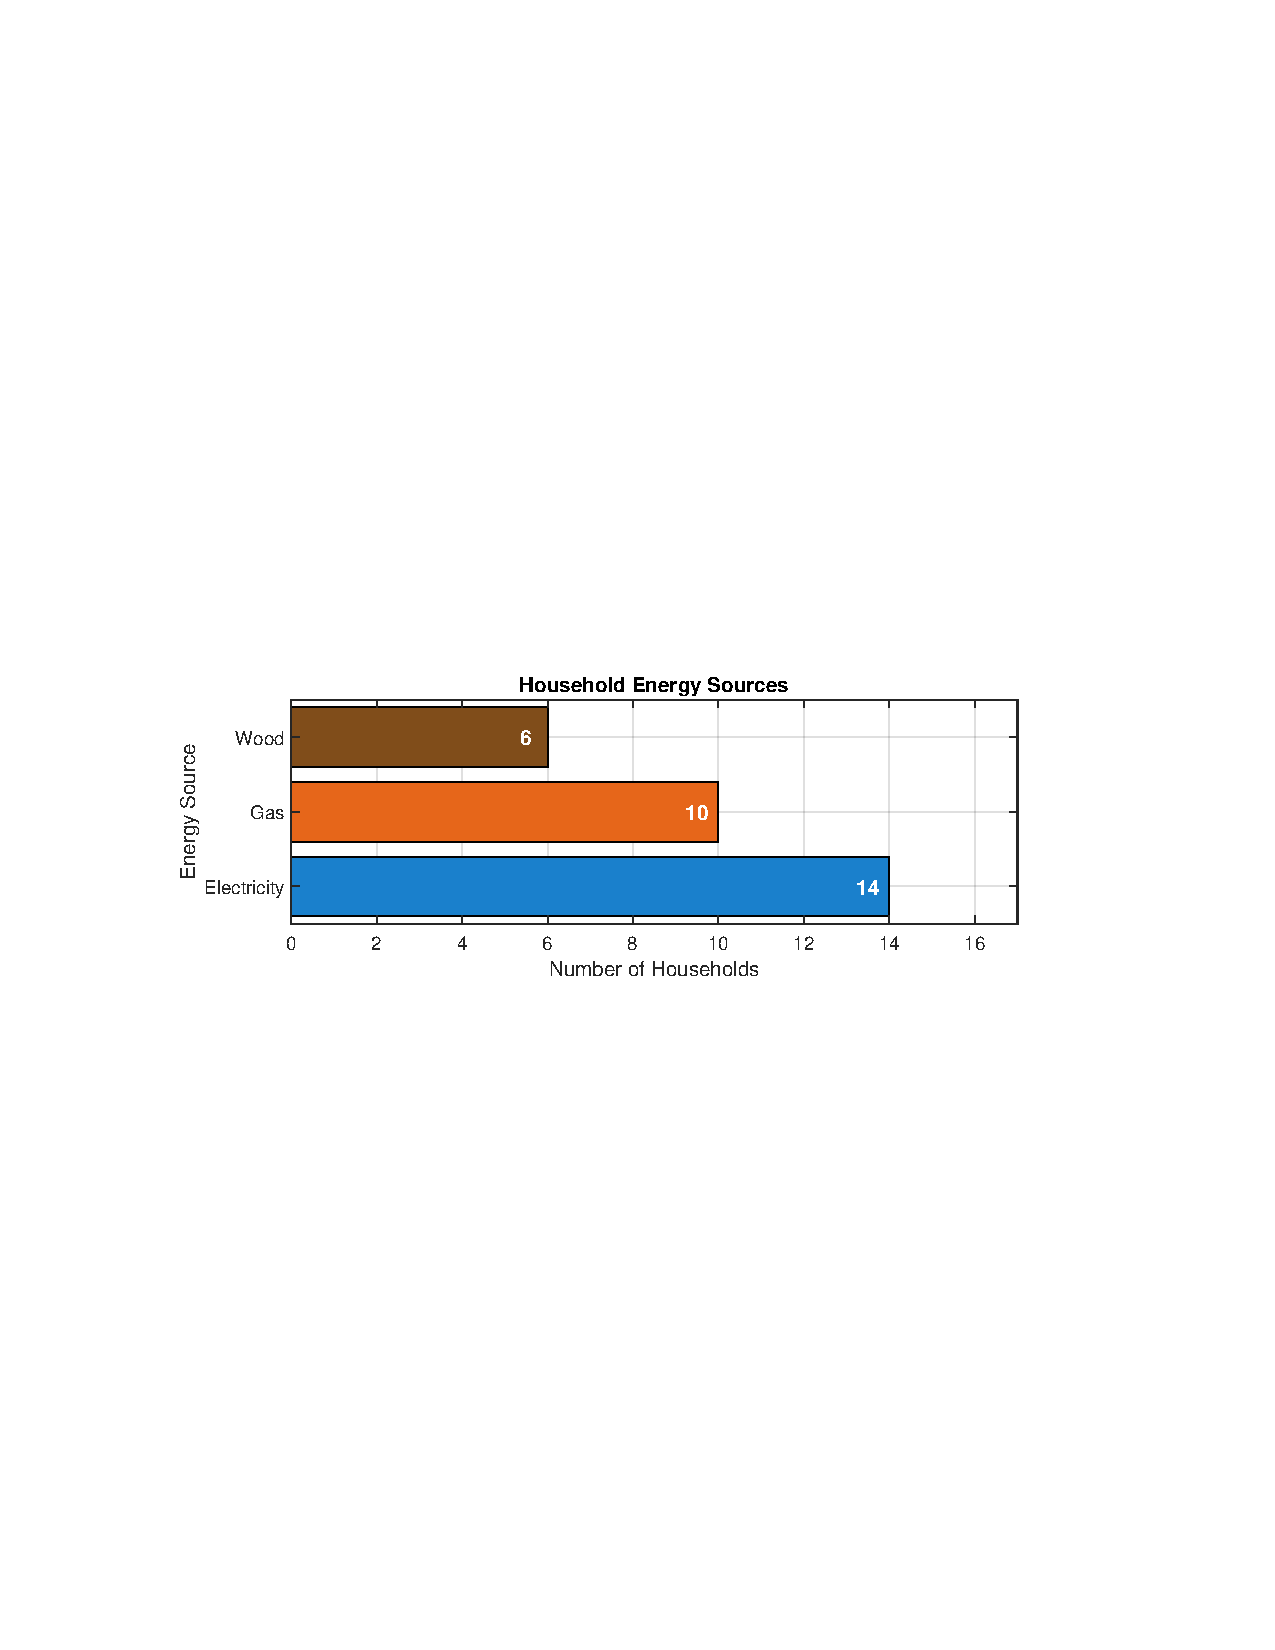
\includegraphics[width=\textwidth]{photos/HouseholdEnergySources.pdf}
        \caption{Numbers are based on 15 interviews of 17 households. Energy sources had various uses, which are not defined here.}
        \label{res:soc:householdenergysources}
    \end{subfigure}
    \hfill
    \begin{subfigure}[b]{0.48\textwidth}
        \centering
        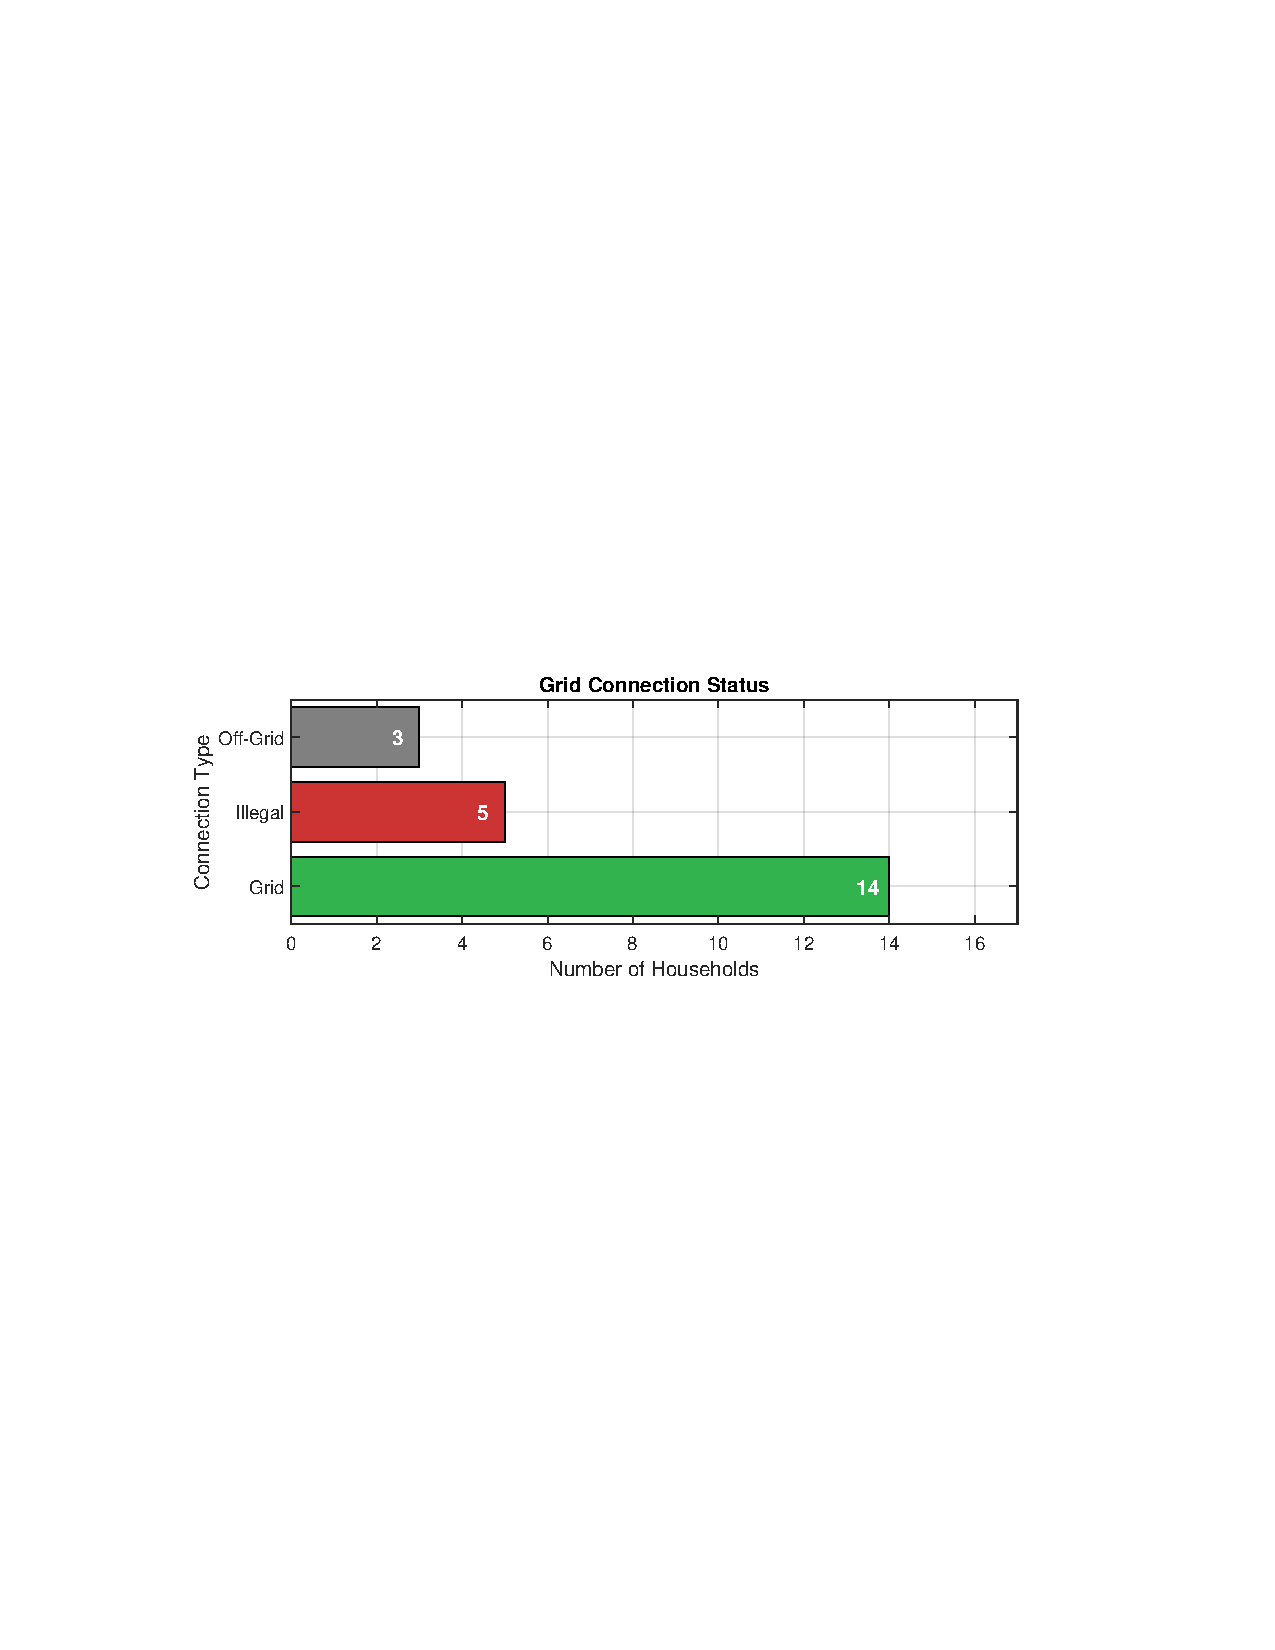
\includegraphics[width=\textwidth]{photos/GridConnection.pdf}
        \caption{Numbers are based on 15 interviews of 17 households. All illegally connected participants where classified as connected to the grid.}
        \label{res:soc:gridconnection}
    \end{subfigure}
\end{figure}
From the graph we see that there were several households that were connected illegally, and some of them were not connected at all. All households that were illegally connected had failed to pay their electricity bill. Either with late payments, or generally incapable of paying for electricity beyond their necessities. Most households had one other energy source than electricity from the grid. Participants viewed the SHS as a separate energy source of electricity. Gas was often used for heating of water and for cooking. Wood was used for general heating or cooking. Most used electricity for washing clothes, TV, sometimes cooking, and sometimes heating water for showers. Among the ones off-grid, two of them were families that had grid connection in the household but were using it for lighting in a shed that had no connection. Two of the illegally connected households had recently connected themselves to the grid illegally, and was previously without electricity. 

\subsection{Power outages and candles}
During the interviews, participants often mentioned regular power outages. Even though we didn't have this as a specific question, we commonly asked this question. The result can be seen in figure \ref{res:soc:poweroutages}. The same thing happened with the SHS replacing candles. Participants often mentioned it as a positive benefit of the systems, and the results can be shown in figure \ref{res:soc:removedcandles}. 

\begin{figure}[H]
    \centering
    \begin{subfigure}[t]{0.48\textwidth}
        \centering
        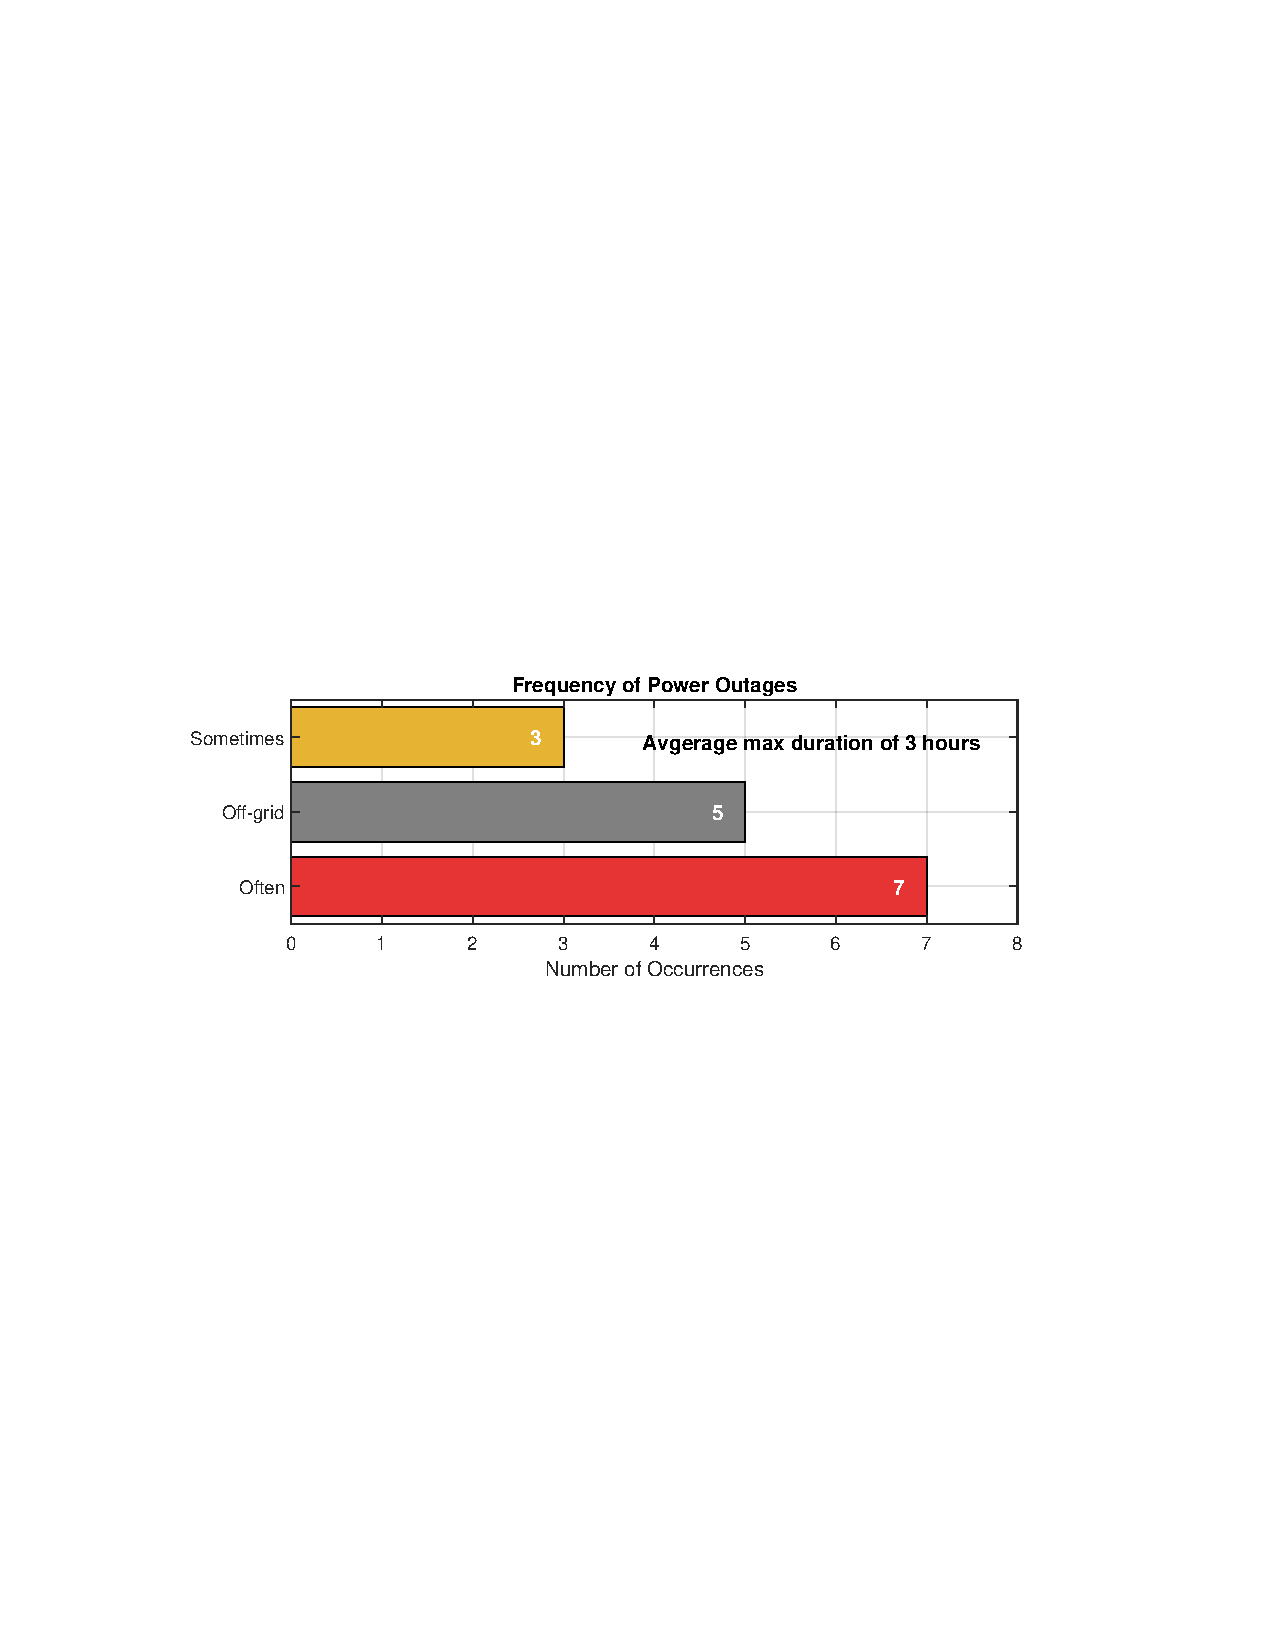
\includegraphics[width=\textwidth]{photos/PowerOutagesFrequency.pdf}
        \caption{"Often" and "Sometimes" are the most accurate data we got from interviews. Some participants referred to often as up to 2-3 times a day. Off-grid are households that had or recently had no grid connection and could not answer for grid stability.}
        \label{res:soc:poweroutages}
    \end{subfigure}
    \hfill
    \begin{subfigure}[t]{0.48\textwidth}
        \centering
        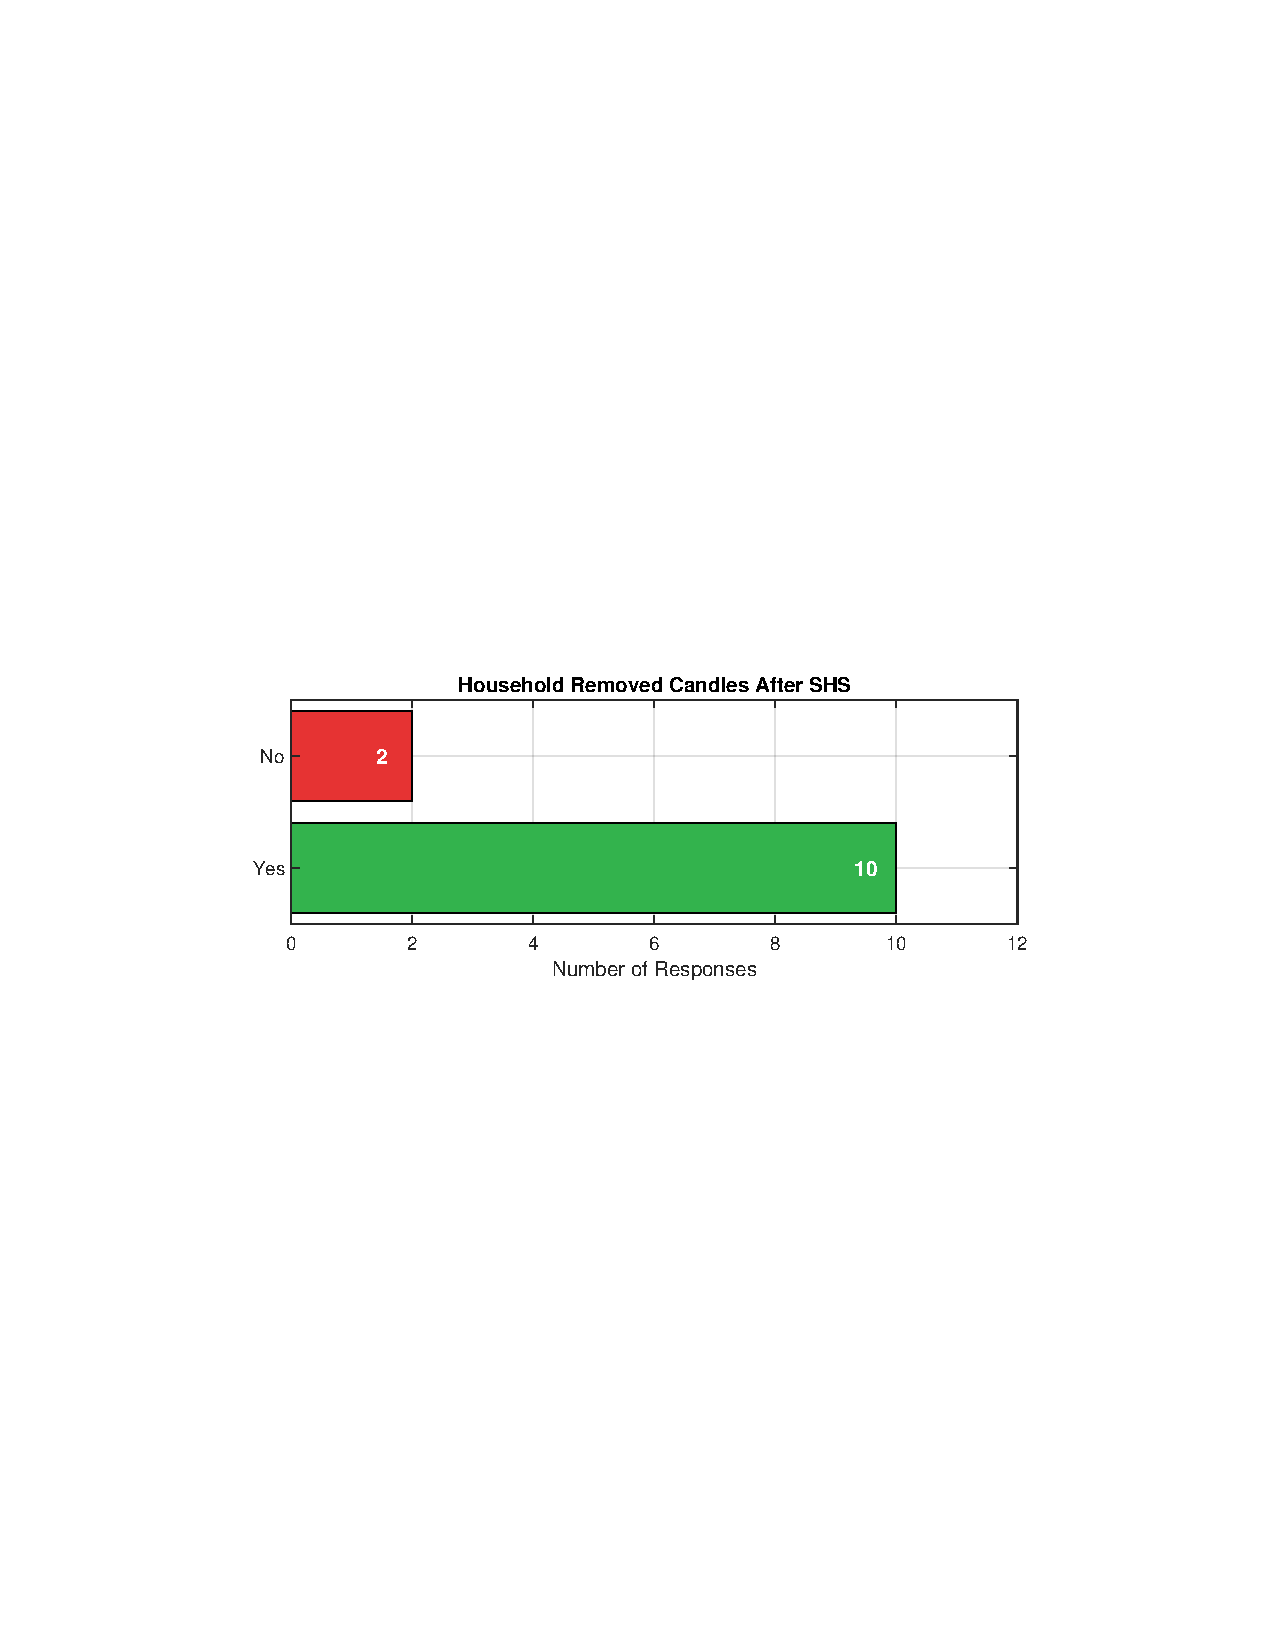
\includegraphics[width=\textwidth]{photos/RemovedCandles.pdf}
        \caption{Based on answers and conversations in interviews. The households that had not gotten candles removed had other systems for emergency lighting, such as battery driven electric lights.}
        \label{res:soc:removedcandles}
    \end{subfigure}
\end{figure}
There seemed to be a high interest for both having an emergency system for power outages, and specifically for being able to removed the need for candles during a power outage. Frequent power outages can create a hard time when having no backup system, and some parts had longer without power than others. Particularly rural areas could have longer power outages than urban areas. One of the main reasons that participants preferred to remove candles, was the fire hazards of having lights inside the house. Participants were acutely aware of the hazards that candles might bring and the consequences of a fire.


\subsection{Household economics}
Participants showed no reluctance to share their incomes and expenditures, giving us the results on figure \ref{res:fig:HouseholdElectricityEconomy}. Some households included more people than others, but this is not shown in the figure. The households are compared regardless of their size, which is why the numbers differ as much. In addition, the numbers for payment reduction are not based on system due to the sample size already being low. 
\begin{figure}[H]
    \centering
    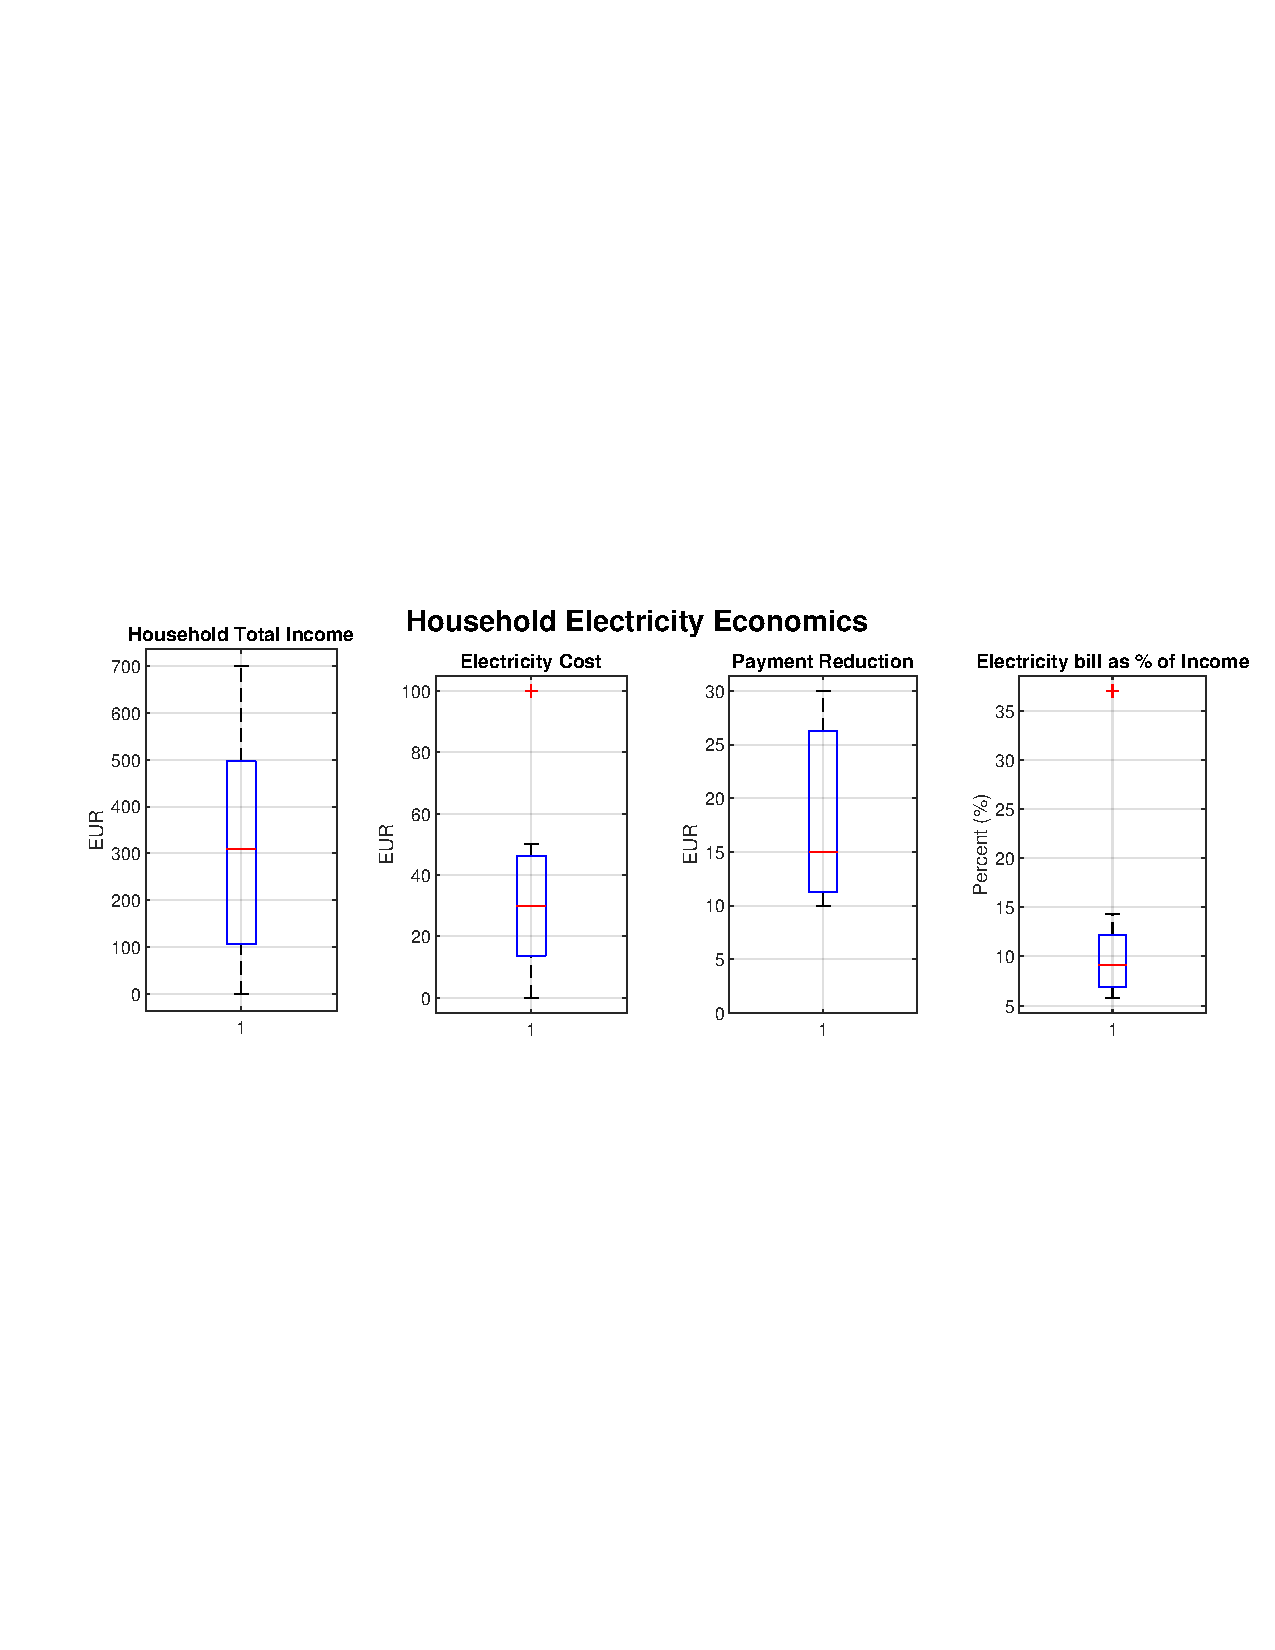
\includegraphics[width=\linewidth]{photos/HouseholdElectricityEconomy.pdf}
    \caption{Box plots of household electricity economy. Numbers are on a monthly basis. Sample sizes are $n=12$, $n=9$, $n=3$ and $n=8$ receptively. Inconsistencies in income and costs sample sizes are due to off-grid and illegal connections, as well as lack of general answers.}
    \label{res:fig:HouseholdElectricityEconomy}
\end{figure}
Total household incomes generally were below 400 EUR a month, which we were told was a normal paycheck for a working person during the field trip. Although not a question asked in the field trip, some people reported how much they had seen a reduction in the electricity bill after installing the SHS. Monthly electricity costs were also taken from a normal month, as the participants often reported being overcharged in the winter months. Some months would charge 5-10 times more than a normal month, based on estimation of consumption and not on actual measurements. This resulted in a complain, which forced the electricity company to measure the correct power consumption and reducing the bill.

Participants showed careful awareness of how much energy they used, taking care not to consume unnecessary energy. The power bill was an average of 8\% of their household income, meaning there was a lot to save on reducing the energy expenditures.

Demographic composition of households in the study differs a lot. Some were elderly people living alone with a pension, and some were families with small children. Figure \ref{res:fig:HouseholdComposition} shows the general composition of a household, and the variation of it. 
\begin{figure}[H]
    \centering
    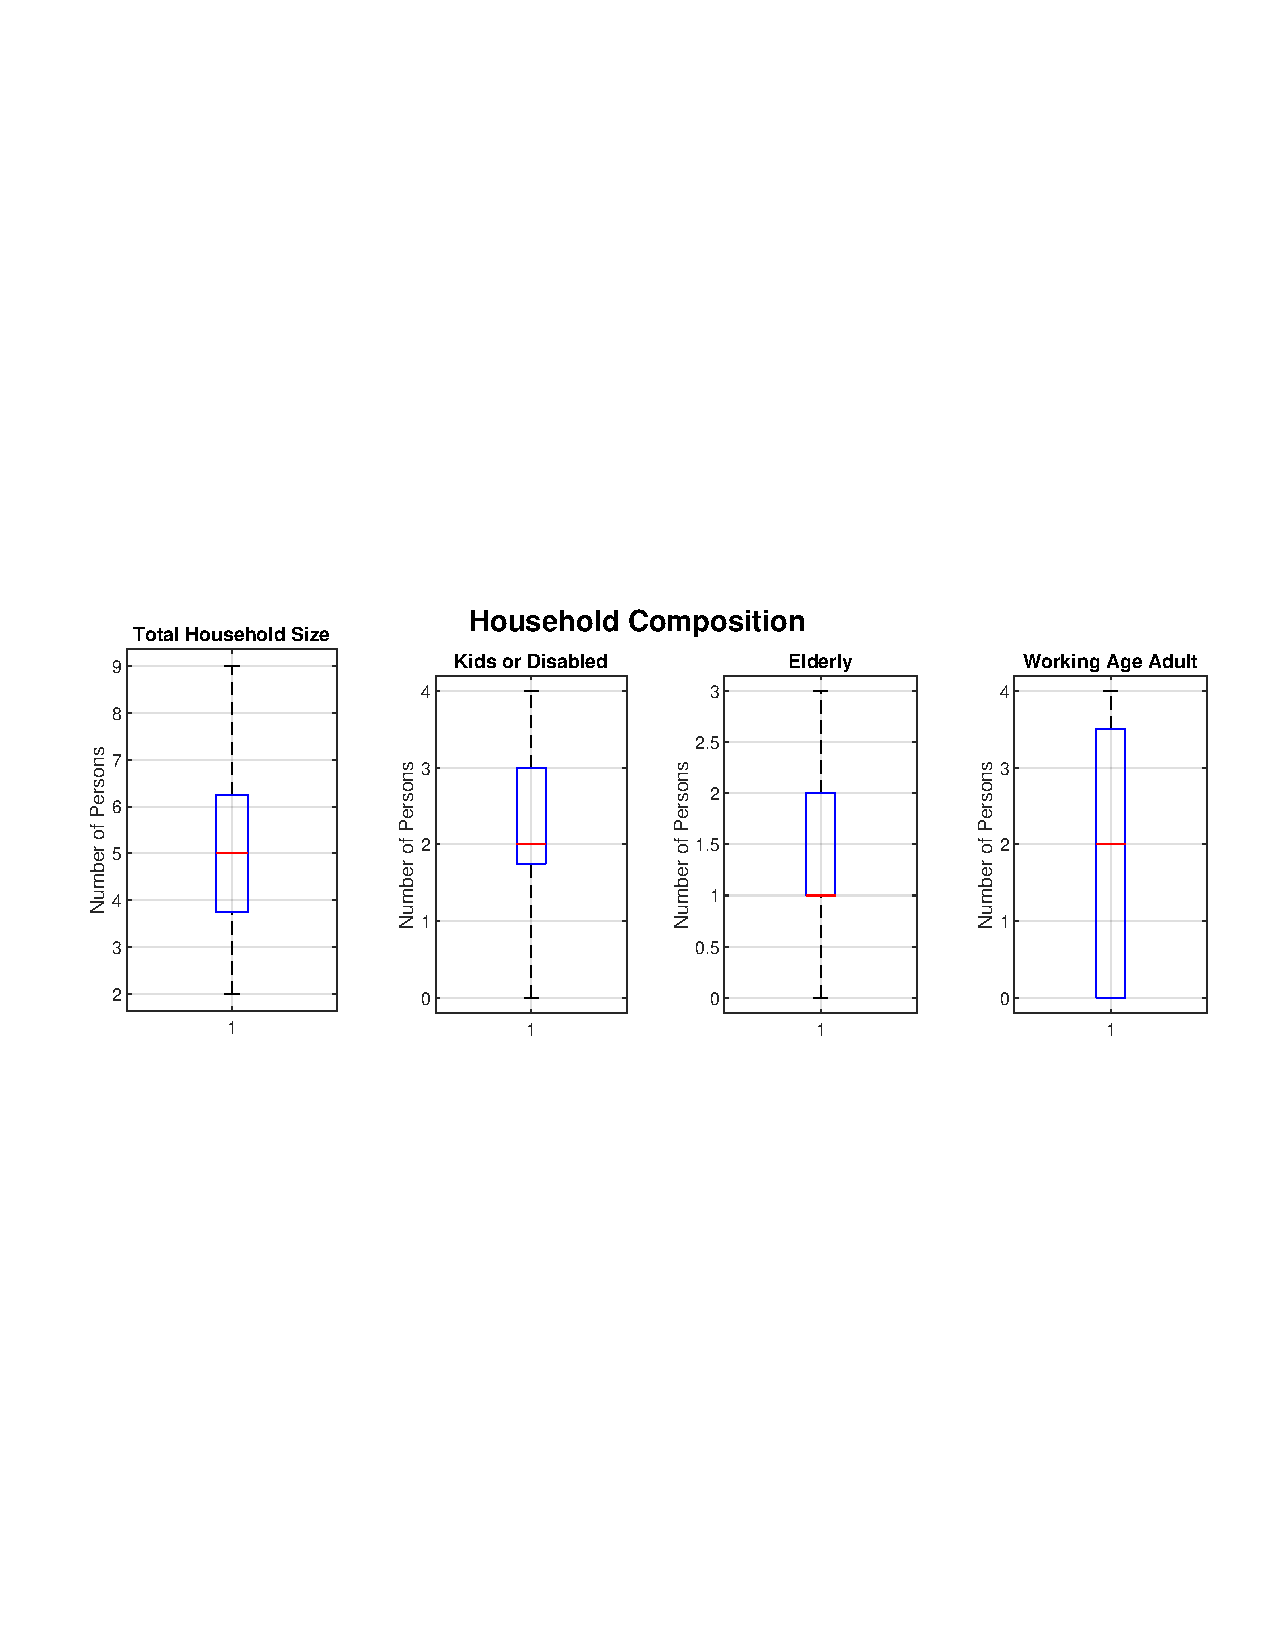
\includegraphics[width=\linewidth]{photos/HouseholdComposition.pdf}
    \caption{Box plots of household composition in terms of kids, elderly and working age adults. Sample sizes are $n=13$ for all plots.}
    \label{res:fig:HouseholdComposition}
\end{figure}
There were several families that included disabled people, as this had been a priority for the project. Households with disabled people reported using the lights throughout the night as a safety in terms of needed care. Small children families often included two adults, where one was working and the other one taking care of the kids. In general there was usually not more than one income per household, besides government support. Most elderly and disabled people received pension from the state as their primary source of income. 

\subsection{Solar power views}
One of the goals of the study was to increase awareness around renewable energy. All of the participants where fond of solar power as an energy source. Most referred to the freedom it had provided them, and how simple it was to use solar power. Contrary to the norm of connecting PV systems to the grid in residential houses, they valued that the system was off-grid. They found the system reliable, and generally understood the concepts of how the solar panel harvested energy for the system. Most people only desired to have more solar power in their household, claiming that they needed a bigger panel. 
%!TEX root = ../thesis.tex

\chapter{Discussion}
\label{ch:discussion}
This chapter aims to represent the data in context with the field trip. Discussing the results given i the previous chapter, this chapter refers to results as it is read fully. Uncertainty of data is cited, and future changes to the study. 
\section{Power simulations}
Tilt angle and azimuth was based on observations. Though fairly accurately described and taken pictures of, the angle is still estimated and individually grouped. No angle measuring instrument was used, and only a simple mobile compass was used to determine the azimuth. As the results show, the tilt angle and azimuth proved to give a significant reduced effectiveness of the panels. Still, not every panel could be placed in an optimal setting. Mounting the system firmly and safely was a greater priority for the installers that helped than the angle and azimuth was. Some of the households did not have the possibility of placing the panel optimally. Shading of the panels were not accounted for, but were generally not common among the participants.

Cleaning was a factor that the receivers was not informed about. In general they got the training they needed for the system, but maintaining the panels by washing was unknown by the local aid organization. All participants got this information during the interviews, and the organization informed other recipients of washing.

Seasonal differences in production and consumption is a simplification of the process that causes inaccuracy. As we did not have data besides what the participants consumed in winter and summer time, using two rigid dataset for consumption on a dynamic production dataset would also cause inaccuracy. Creating two distinct simulations also reduced the inconsistency of weather, as the dataset for irradiance was for 2023. Future studies could use integrated logging technologies to analyze the power data more precisely. SoH for batteries was not measured, as we had to prioritize tasks in our short time. We disregarded SoH estimation as the age would make the deterioration negligible. 

A general loss factor of 14\% could have been unjustified, and to analyze this actual measurements could have been done. As the system is using voltage conversion mechanisms for charging and discharging, the system could be more or less efficient than specified. The simulation should have used the median efficiency loss from azimuth and tilt angle, as only some panels were badly placed. The median reduction was 14\% and could have better represented the normal placement of panels. A soiling loss factor of 10\% could have been more specified based on each panel, but time budget of interviews did not give us the opportunity to inspect the panels closely.

Summer and winter data mostly showed how utilized the systems were. When simulating the combined data against a BH 800 system on figure \ref{result:fig:Winter_40wpp_all_losses}, the system showed complete usage of the produced power. Since the bottleneck is the winter time, this is a optimally sized system for it's use. It should be noted that the general simulations on the BH 800 were made with combing all systems consumption data, which included the data BH 600 and BH 300 systems. Since the sample size was low for each system, this way of combining the datasets could give a more accurate representation of consumption. On the system specific simulations, datasets were not as general as the combined. Simulations on figures \ref{result:fig:300_winter_soc}, \ref{result:fig:600_winter_soc} and \ref{result:fig:800_winter_soc} showed how each system was fully utilized in the winter. As the participants did not state that the battery would empty each day, there is a mismatch between the data. Most likely the consumption data is overestimated. Causes for the mismatch could be inaccurate descriptions in interviews, or inaccurate assumptions done during the structuring of the interview data.  


% Du kom hertil
\section{Economic}
Although section \ref{ch:back:sec:solar} refers to an LCOE of 0.044 USD per KWh, this does not directly apply to a SHS. The system includes lights, battery and is customized to a user friendly size. These functionalities are not included in a utility-scale PV system. Lower LCOE in utility-scale PV systems point towards a trend of declining costs of solar technology, which will benefit SHS in the future. As table \ref{tab:lcoe_qty_cons_5_condensed} with 5\% discount and consumption data shows, the LCOE is still around 20 EUR/kWh for the stated lifetime. Cost of electricity from the grid is 0.12 EUR/kWh, giving SHS 100 higher cost per unit of energy. This is partially from the low cost of electricity in Albania, being half of what the EU-27 average is. Rising electricity price could increase the profitability against the LCOE and payback time, but there was no real basis to predict this on a 6-7 years lifespan.  If one were to do a more fair analysis of the cost, the benefits of the utility should be considered and removed from the investment cost. The systems includes lighting sources, which would otherwise have had to be bought. For off-grid households or buildings, this can be a costly process that makes a SHS be the most affordable solution. Although the systems are marketed to a 6-7 years life cycle, it is likely that they will last longer. SHS are typically estimated to live for longer, being based on lifetime of battery. As section \ref{chap:method:sec:LCOE} explain, the lifetime of a battery can be up to 9000 cycles or about 24-25 years. This would reduce the LCOE to about 7.5 EUR/kWh when using consumption data and 5\% discount rate. 

Users would still give a high price for the system even though the pure economical payback time would be higher than a worthwhile investment. From the payback time in figure \ref{result:fig:paybacktime}, they would still have minimum of 25 years for a economical payback in terms of energy bill reduction. This shows that there are benefits beside the economical that the participants value. 

Overcharging was reported by almost all participants. \citep{likmeta2007} reports this as a problem as far back as 2007. The problem seems to be a know issue, and likely due to missing measurements of electricity consumption. When overcharging is that normal, Albanians may feel unease by being connected to a grid without control of their costs. Suddenly being charged five times higher than normal for power could break a fragile household economy. \citep{Hejsek2011} reports that some people where using power lavishly without seeing a change in the power bill, as the bill was estimated anyway. Even though we were there to interview about the SHS, participants expressed their frustration of the power system in response. Participants expressed a desire to be self-sufficient as solution against the overcharging from the electricity companies. Most then referred to a bigger SHS as the step towards this, although none had the means to invest in this.

\section{Social}
Participants reported that the system gave them freedom to use their own electricity, not reliant on the grid. This could have been because of the common power outages that often lasted a while, giving them a sense of control that they lacked without the system. Several reported feeling an increased safety with the system, giving them an emergency solution in a power outage. Illegally connected households particularly reported feeling safer with the system, knowing they had a backup system if they were to be disconnected from the grid. As gas and wood was a common energy source for cooking and heating water, electricity was mostly used for lighting, TV and washing clothes. The SHS would then be able to cover the need of lighting and phone charging, making the situation less critical than it would be without it.

One interviewed household was off-grid, where there was seven people in the household. They used only the SHS as light in addition to rechargeable electric lights where the lamps could not reach. Rechargeable lights were being charged by using the USB-A port on the SHS. Additionally, they charged a power bank to serve as extended battery capacity for the SHS. The household had grid infrastructure, meaning they choose not to connect to the grid. The two off-grid sheds had grid connection inside the household, but had not extended this into the shed. Participants with sheds explained that they would otherwise not have had electricity in the building, as the cost of extending the power was too costly. 

Power outages were common among the participants. Being frequent and lasting for a while, participants reported this being a source of worry. \citep{giz_kfw_2013}, a german organization working in Albania - took the measure of installing a EUR 20,000 system to elude the issue of power outages in the capital. Some rural areas were exposed to longer power outages than urban. Some reporting that there could be a day before they would get power again. Specially households with disabled and elderly valued that the system was independent of the grid. Having lights available in power outages made care easier. Participants reported using the light as a safety during the night, but had not used this previously in fear of high electricity costs. The social house reported that this allowed them to have meals in a power outage, where they previously had to cancel. Using rechargeable lights as their backup, this was not enough light to safely arrange meals. The SHS also served as an important safety for both the patients and the caretakers, as there was no emergency generator for the building.

Candles were the most common alternative to lighting during power outages. The use of candles is as mention in section \ref{ch:metod:powerout} connected to fire hazards. Participants were aware of the risk, and often cited removing the use of candles as one of the best use cases of the system. As removing candles was not an original question we had before the field trip, the participants were actually the ones that consistently brought this up. \citep{obengSolarPhotovoltaicElectrification2008} in Ghana cites PV systems as reducing the indoor smoke from kerosene lamps, and replaces the need for candles. Although the literature is referring to off-grid areas, frequent power outages create the need for alternative lighting sources like candles and kerosene lamps. \citep{Sinoruka2023} tells the story of a village in rural Albania that previously did not have street lamps, using torches for lights at night. Now they have gotten a PV system for their streetlamps, giving them light throughout the night.

Households reported a higher electricity payment reduction in figure \ref{res:fig:HouseholdElectricityEconomy} than the system would generate in terms of power. With the lowest reported saving of EUR 10, this is still above the optimally generated power price from any system. With three data samples, it is too uncertain to claim cost saving. Participants did seem to expect an energy saving from the system though, as we did not ask the participants of energy savings from the system. In fear of it being a leading question, we instead asked about consumption and energy costs. Participants were particularly aware of their energy costs, and took care to save energy where they could. 


\section{Organizational}
Local aid organization The Door Albania had selected the receivers of the SHS. From their work they had a network of receivers of aid, which they used select the participants of the project. In addition, they had dialogue with the municipality of Shköder to find more participants. The organization had a detailed list of the participants of the project, and served as a contact for the system. Participants knew that if there was an issue with the system, or if they needed training - the organization would help them. Participants often received additional help from the organization besides the SHS, and had regular communication. 

This way of structuring the aid seemed to be successful. \citep{chaureyAssessmentEvaluationPV2010} cites that the attitude of the user determines the success of the program, and the significance of local involvement in programs. Having this project driven by an established local aid organization could make participants feel more responsibility for the systems. During interviews, participants exclaimed their gratefulness for the systems and often thanked the organization. 

\section{Shortcomings}
The general shortcoming of this thesis is the number of variables gathered for the social evaluation. There is no value in gathering more data for the economical analysis, as this can be concluded with the data we have gotten. The data on SHS outside of off-grid areas is low, due to few projects being done in this area. Narrowing down on the social effects that the systems give would be the way forward. The study could have more data points within an even more narrow category. Some interviews were done in a social housing complex, where the municipality had put up modular units for poor families. This place had over 20 families with systems of which we only got to interview three in our time there. Narrowing down the sample group to only these would give more precise data. Nevertheless, the data we got should accurately represent the entire selection. As there were 187 systems given with 14 of them being reserves, we interviewed for over 1/10 of the systems. 

This study does not include data from other developing middle-income countries. Comparing the results of this study with other projects in developing countries with high grid coverage would be the next step for research in this field. Particular points of interest would be organizational, social, cultural and grid infrastructure. 

%!TEX root = ../thesis.tex

\chapter{Conclusions}
\label{ch:conclusion}

The findings of this paper suggest that the benefits of SHS in developing middle-income countries with high grid coverage are mostly social, as opposed to economical. With payback time of over 50 years and LCOE of 19.7-26.5 EUR/kWh, the economical benefits of a SHS are negligible compared to the cost. SHS are fully utilized, consuming all of the electricity that they produce in winter time and generating a surplus in the summer time. Users show high interest in the systems, taking good care of the system and treating it as valuable. People particularly valued their systems as a backup in case of power outages, which were frequent in Albania. Some were illegally connected due to not being able to pay the electricity bill, and risked being disconnected at any time. Even with full grid coverage, there are still off-grid uses for a SHS - including sheds and households disconnected from the grid. Common alternative sources of energy such as gas and wood were used for cooking, hot water and heat - making the SHS fill the remaining need for lighting and charging electronics during power outages. Using a local organization for managing a SHS project was successful, giving participants a contact for maintenance and training. 

A potential area of further research is to further investigate the social benefits of having a solar powered backup system for households in countries with low grid stability. 

%-----------------------------------------------------------------
% Now begin the Appendices, including them as separate files

% \listoffigures
% \listoftables

\appendix
%!TEX root = ../thesis.tex

\chapter{Supplementary theory}
\label{ch:theory}

\section{Solar Home System}
Solar home systems exist in various different sizes to address different needs. Common for them all are that they are stand-alone systems, designed to be implemented into a single household. Not being attached to the grid, their main purpose is to generate and store enough electricity during the daylight. Hopefully storing enough energy in the batteries to power lights or other appliances until the next light comes again. This cycle is demonstrated in figure \ref{fig:SHS_drawing}.

\begin{figure}[h]
    \centering
    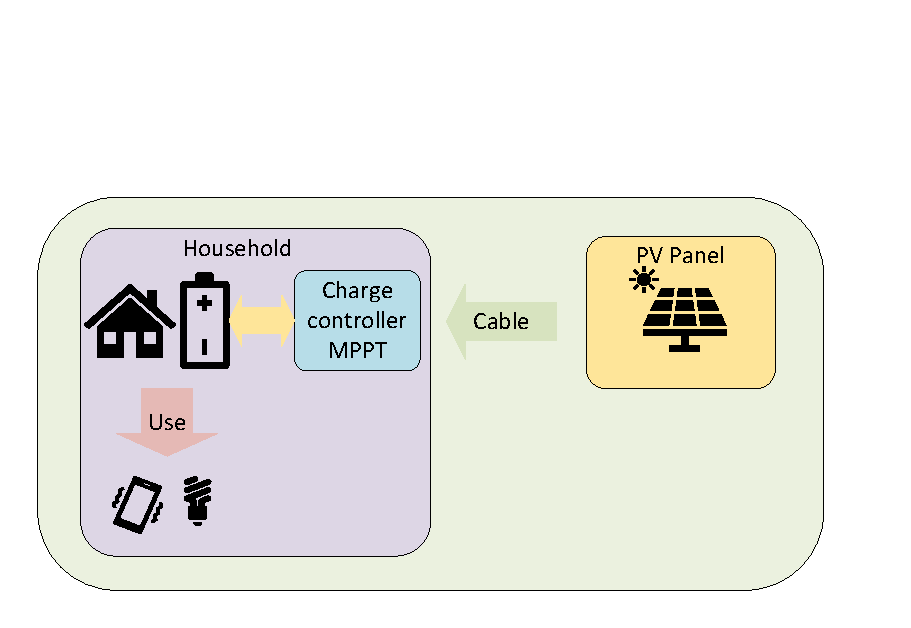
\includegraphics[width=\linewidth]{photos/SHS_drawing.pdf}
    \caption{Solar Home System connection}
    \label{fig:SHS_drawing}
\end{figure}

The PV panel will provide a voltage to the charge controller, which will charge battery. The battery will then supply low power appliances like phones and lights. 

To perform optimal charging, a \acrfull{mppt} controller is used. The controller finds the optimal voltage to current ratio for charging based on the voltage from the PV panel. This ensures optimal charging even when the PV panel does not have optimal conditions, such as shading, low sun or dirt on the panel.

\subsection{Power generation}

\subsubsection{Photovoltaic}
For photovoltaic cells to capture energy from light sources, they need to absorb photons into their silicon wafer. When a photon is absorbed in silicon, its energy is transferred to an electron. This process is what makes it possible to transform light into usable electric charge. How many photons that enter this wafer is what decides how much energy the PV module will capture. Factors like irradiance, angle and temperature change how many photons get absorbed \citep{wirthPhotovoltaicModulesTechnology2016}.

\subsubsection{Irradiance}
The number of photons that hit an area\footnote{Called the quantum flux}, will decide the amount of irradiance. Irradiance will rise during a day, ending up with being strongest when the angle of the sun is perpendicular to the surface it shines against. Since the angle the sun will have on the earth changes during the year, the actual irradiance will also change correspondingly. Affecting parts further from equator more than those closer, seasonal variations will increase or reduce daily irradiance. Light will scatter more in a low hanging winter sun than when given a long lasting summer sun. Weather variations will also change the way light scatters. Cloudy weather will give a reduced amount of irradiance, while clear low humidity weather will give more irradiance. 

To estimate irradiance, we can use formulas or simulations. These being created on the angle of the sun and weather variations, we can find an accurate representation of the actual conditions. 

\subsubsection{Solar panel}
Solar panels will have a wattage peak effect, limiting how much energy they can absorb in the solar cells. Larger panels will absorb more sunlight, creating more electricity. To account for the direction of the sun, having an angle on the solar panel will give an increased irradiance.

Solar panels have varying amount of loss, but one way of analyzing the performance ratio of the module is equation \eqref{eq:performanceratio}.

\begin{align}
    PR_{mod} & = \frac{E_{DC}}{H_{POA}A_{MOD}\eta_{STC}}
    \label{eq:performanceratio}
\end{align}
Where:
\begin{itemize}
    \item $PR_{MOD}$ is annual module performance ratio
    \item $E_{DC}$ is annual som of delivered energy assuming MPPT $[MJ]$
    \item $H_{POA}$ is annual irradiation into plane of the module $[MJ/m^2]$
    \item $A_{MOD}$ is total module area $[m^2]$
    \item $\eta_{STC}$ is module efficiency under standard test conditions (STC).
\end{itemize}

To find this, we need to know the performance module efficiency. This is measured during standard conditions of 1000 $W/m^2$ and \SI{25}{\celsius}. See equation \eqref{eq:panelefficiency}

\begin{align}
    \eta_{mod} &= \frac{P_{mod}}{E_{STC}A_{mod}}
    \label{eq:panelefficiency}
\end{align}
Where:
\begin{itemize}
    \item $\eta_{mod}$ is the module efficiency
    \item $P_{MOD}$ is maximum power point
    \item $E_{STC}$ is irradiance at standard test conditions
    \item $A_{MOD}$ is total module area $[m^2]$
\end{itemize}

\subsubsection{Soiling}
Soiling on the panel will cover the modules, hindering photon absorption and reducing module efficiency. Soiling can come from several pollutants such as ash, stone dust, sand, coal powder or cement. Panels get more contaminated based on how much upward-facing surface it has. Equation \eqref{eq:dustreduction} shows the relationship between the tilt angle and the upward-facing surface based on \citep{yakubuHolisticReviewEffects2025}.

\begin{align}
    St & = A \cdot \cos{\alpha}
    \label{eq:dustreduction}
\end{align}
Where:
\begin{itemize}
    \item $St$ is the upward-facing surface
    \item $A$ is the module area 
    \item $\alpha$ is the tilt angle
\end{itemize}
\citep{yakubuHolisticReviewEffects2025} found soiling to reduce the effect from 10\% in mild regions, up to 40\% in arid regions. Manual cleaning showed to restore up to 98\% of the module efficiency. 

\subsubsection{Tilt angle and Azimuth}
When using fixed tilt\footnote{The alternative to fixed tilt is solar tracking, where the panel will adjust itself in coordination with the sun.}, the panel should face the south when in the northern hemisphere. \citep{SolarEnergyEngineering2024} shows that for maximum annual production, the optimal tilt angle can be found using equation \eqref{eq:tiltangle}

\begin{align}
    \alpha & = 0.764L \ + \ 2.14^\circ, for \ L \leq \ 65^\circ
    \label{eq:tiltangle}
\end{align}
Where:
\begin{itemize}
    \item $L$ is the latitude
    \item $\alpha$ is the tilt angle
\end{itemize}

\citep{SolarEnergyEngineering2024} also proposes adjusting for afternoon sun, when the demand is higher. This would mean adjusting the angle higher to capture a low afternoon sun. For a SHS, this can make sense when wanting it fully charged for the night. 

Another factor is the azimuth\footnote{Azimuth is the horizontal angle of a cardinal direction, often south or north. In this case, we use the PVGIS definition of \SI{0}{\degree} azimuth to be south.} of the panel. The most common angle in the northern hemisphere is to use \SI{0}{\degree}, although you can apply the same principle of adjusting for afternoon sun here as well. Fixing the azimuth more towards the setting sun on the east would give more irradiance from a setting sun. This will unfortunately greatly affect production during peak-hours.
\subsection{Battery}

\subsubsection{State of Health}
A battery's \acrfull{soh} will give an indication of how effective a battery is based on how much charge it can hold compared to a nominal charge. The SoH will be reduced by during the lifetime of the battery. Time, high or low temperature, high or low voltage and high current rate will degrade the SoH\citep{liuDataScienceBasedFullLifespan2022}. To find the SoH of a battery, we can use equation \eqref{eq:soh}. This equation will give us two ways to measure the SoH, either using the charge or using the internal resistance. 

\begin{align}
    SoH_{C} &= \frac{C_a}{C_n} \cdot 100\%  \\
    SoH_R &= \frac{R_a - R_r}{R_r} \cdot 100\% 
    \label{eq:soh}
\end{align}
Where:
\begin{itemize}
    \item $C_a$ is actual charge
    \item $C_n$ is nominal charge
    \item $R_a$ is actual internal resistance
    \item $R_r$ is rated internal resistance
\end{itemize}

To find the actual internal resistance, we can apply a known load to the battery and measure before and after the load is applied. This will give us the voltage split over the two resistances, and using ohms law we can find the internal resistance of the battery. 

\subsubsection{Lifetime}
The type of battery and the conditions it is exposed to determines the lifetime\footnote{The lifetime of a battery is when it reaches 80\% of the initial capacity it had} of the battery. On off-grid PV systems, \citep{wieczorekInfluenceCurrentOffgrid2023} found \acrfull{lfp} batteries to be the most lasting when given incomplete charges. In the worst cases having a lead-acid battery last for 30 cycles before reaching it's end of life. 
\subsection{Consumption}

\subsubsection{LED}
\acrfull{led} is a light technology that consumes less energy per lumen than incandescent light bulbs. \citep{usdepartmentofenergyLifeCycleAssessmentEnergy2012} claiming that LED is about one quarter of the energy consumption of incandescent lights per functional unit\footnote{Functional unit is defined as 20 million lumen hours}. The evaluation was done as a life cycle assessment, meaning they looked at the entire process and not just compared power rating and lumen. In terms of lumen per energy unit, \citep{podeLightEmittingDiodes2011} claim LED saves 80\% energy compared to incandescent lighting. 

\subsubsection{Charge port}
\acrfull{usba} is a general interface that is normal for power transfer on phones and other small devices. The standard voltage transfer is 5V, and reaches up to 900mA \citep{jimmylinGettingBottomUSB2021}.

\section{Economic metrics}
\subsection{Levelized cost of energy}
\acrfull{lcoe} is used as a benchmark to determine the cost-effectiveness of different energy generation technologies\citep{brankerReviewSolarPhotovoltaic2011}. The metric uses the lifetime of the equipment, it's cost and the generated energy to estimate a price per unit of energy. The formula of LCOE is show in equation \eqref{eq:LCOEfirst}, which is an expansion of the \acrfull{npv} calculation. When using NPV we also need to introduce a discount rate for the investment and income.

\begin{align}
    LCOE & = \frac{NPV(Costs)}{NPV(EnergyIncome)} \notag \\
    \notag \\
    LCOE &= \frac{\Sigma_{t=0}^T  C_t/(1+r)^t}{\Sigma_{t=0}^T  E_t/(1+r)^t}
    \label{eq:LCOEfirst}
\end{align}
Where:
\begin{itemize}
    \item $C_t$ is net cost of system for t
    \item $E_t$ is energy produced for t in monetary value
    \item  $r$ is discount rate
    \item $T$ is lifetime of the system
\end{itemize}

When $t=0$ we will have our initial cost included into the net cost of the system. $C_0$ will include both the investment cost and any running costs related to the system. To analyze how worthwhile this investment is, the discount rate needs to be compared to a similar investment and it's expected rate. The calculation of $E_t$ will also be twofold, both the energy yield and the actual energy price. A higher price will give a higher LCOE for the given $t$. Based on the lifetime of the system, we will have a higher LCOE as long as the running costs are low. 

\subsection{Discount rate}
Typically the discount rate is calculated from a purely economical perspective, but for renewable projects \citep{sarahleeUltimateSocialDiscount2025} suggest using \acrfull{sdr}. These rates include the long term benefits such as the effect the renewable energy has on the environment for future generations. \citep{sarahleeUltimateSocialDiscount2025} refers to Ramsey Formula to calculate the SDR, here given in equation \eqref{eq:ramseyformula}.

\begin{align}
    r & = \delta + \eta g
    \label{eq:ramseyformula}
\end{align}
Where:
\begin{itemize}
    \item $r$ is the discount rate
    \item $\delta$ is the pure time preference
    \item  $\eta$ is the elasticity of marginal utility of consumption
    \item  $g$ is the growth rate of per capita consumption
\end{itemize}


\subsection{Life cycle cost}
Similar to LCOE, \acrfull{lcc} will analyze the cost of the system for it's lifetime. The difference is that it will not look at the yield of energy, and only focus of the cost of the product\citep{tonioloLifeCycleThinking2020}. \acrshort{lcc} can be used for a simple analysis of the product in terms of initial purchase, or it could take into account the cost of design, production, transport and end life\citep{tonioloLifeCycleThinking2020}. This means we have to decide what is right for this project to apply the method of \acrshort{lcc}. The conventional method to apply \acrshort{lcc} is to assess all the costs during the life cycle of the product\citep{tonioloLifeCycleThinking2020}. Not being structured by an \acrfull{iso} procedure, the method for calculating the \acrshort{lcc} is subject to interpretation and does not have a specific equation. 


\subsection{Payback time}
Payback time is how long it will take accumulated annual revenue to be equal to the initial investment. This is a simple way to calculate how long it will take for a project to be profitable without including any internal rate of return\citep{dahlquistPrinciplesFinance2022}. This is show in equation \eqref{eq:payback}.

\begin{align}
    Payback\ Period = \frac{IC}{R_n}
    \label{eq:payback}
\end{align}
Where:
\begin{itemize}
    \item $IC$ is initial cost at first year
    \item $R_n$ is annual revenue stream for any year
\end{itemize}

The payback period does not take into account any maintenance costs or end of life costs of the investment. Although to fix this, we can incorporate the costs using only marginal revenue as revenue. As there is no expected costs with the SHS, we will assume that revenue will be equal to marginal revenue.  



\chapter{Field Trip Questions}
\label{apx:ftquestions}
{\footnotesize
\textbf{Interview questions:}
\begin{enumerate}
    \item How many do you live with, and what age are they?
    \item Which energy resources do you use (like electricity, gas, oil or others)?
    \item What do you and household use electricity for?
    \item On the SHS, how long do you keep the lights on daily, what power setting, and when do you use them?
    \item On the SHS, how many hours do you charge your phone daily, and when do you do it?
    \item Does the battery ever run out, and what does it take to happen?
    \item Do you use the system for anything else than lighting and phone charging?
    \item What is your electricity price?
    \item What is your income situation?
    \item How did you choose where to put the system, and where is it?
    \item Has there been any issues with the system, and is it time consuming to maintain - if so how many hours?
    \item Is the system simple enough to use, or would you want more training?
    \item How has it affected life in the household?
    \item What are the best use cases you have experienced?
    \item What do you think a fair price for this product would be if you were to buy it now?
    \item Who would you recommend it to, if anyone?
    \item What are your thoughts on solar power as an energy source?
\end{enumerate}
\textbf{Added mid field trip:}
\begin{enumerate}
    \item How frequent and how long are power outages?
    \item Have you replaced candles after receiving the system?
\end{enumerate}
\textbf{Specifically noted observations:}
\begin{enumerate}
    \item System placements, tilt angle and azimuth
    \item Type of system
\end{enumerate}}
\chapter{Matlab}
\label{apx:matlab}
All figures, citations, and matlab code is included in the repository. No raw identifiable data is included there, as the privacy of the participants is protected. 
\href{https://github.com/Jodlar98/Master-Thesis}{Github Thesis Repository}

The Simulink model used to simulate the state of charge on the battery. The model used for battery is taken from Simscape's \href{https://se.mathworks.com/help/simscape-battery/ref/batterycccv.html}.{Battery CC-CV}
\begin{figure}[H]
    \centering
    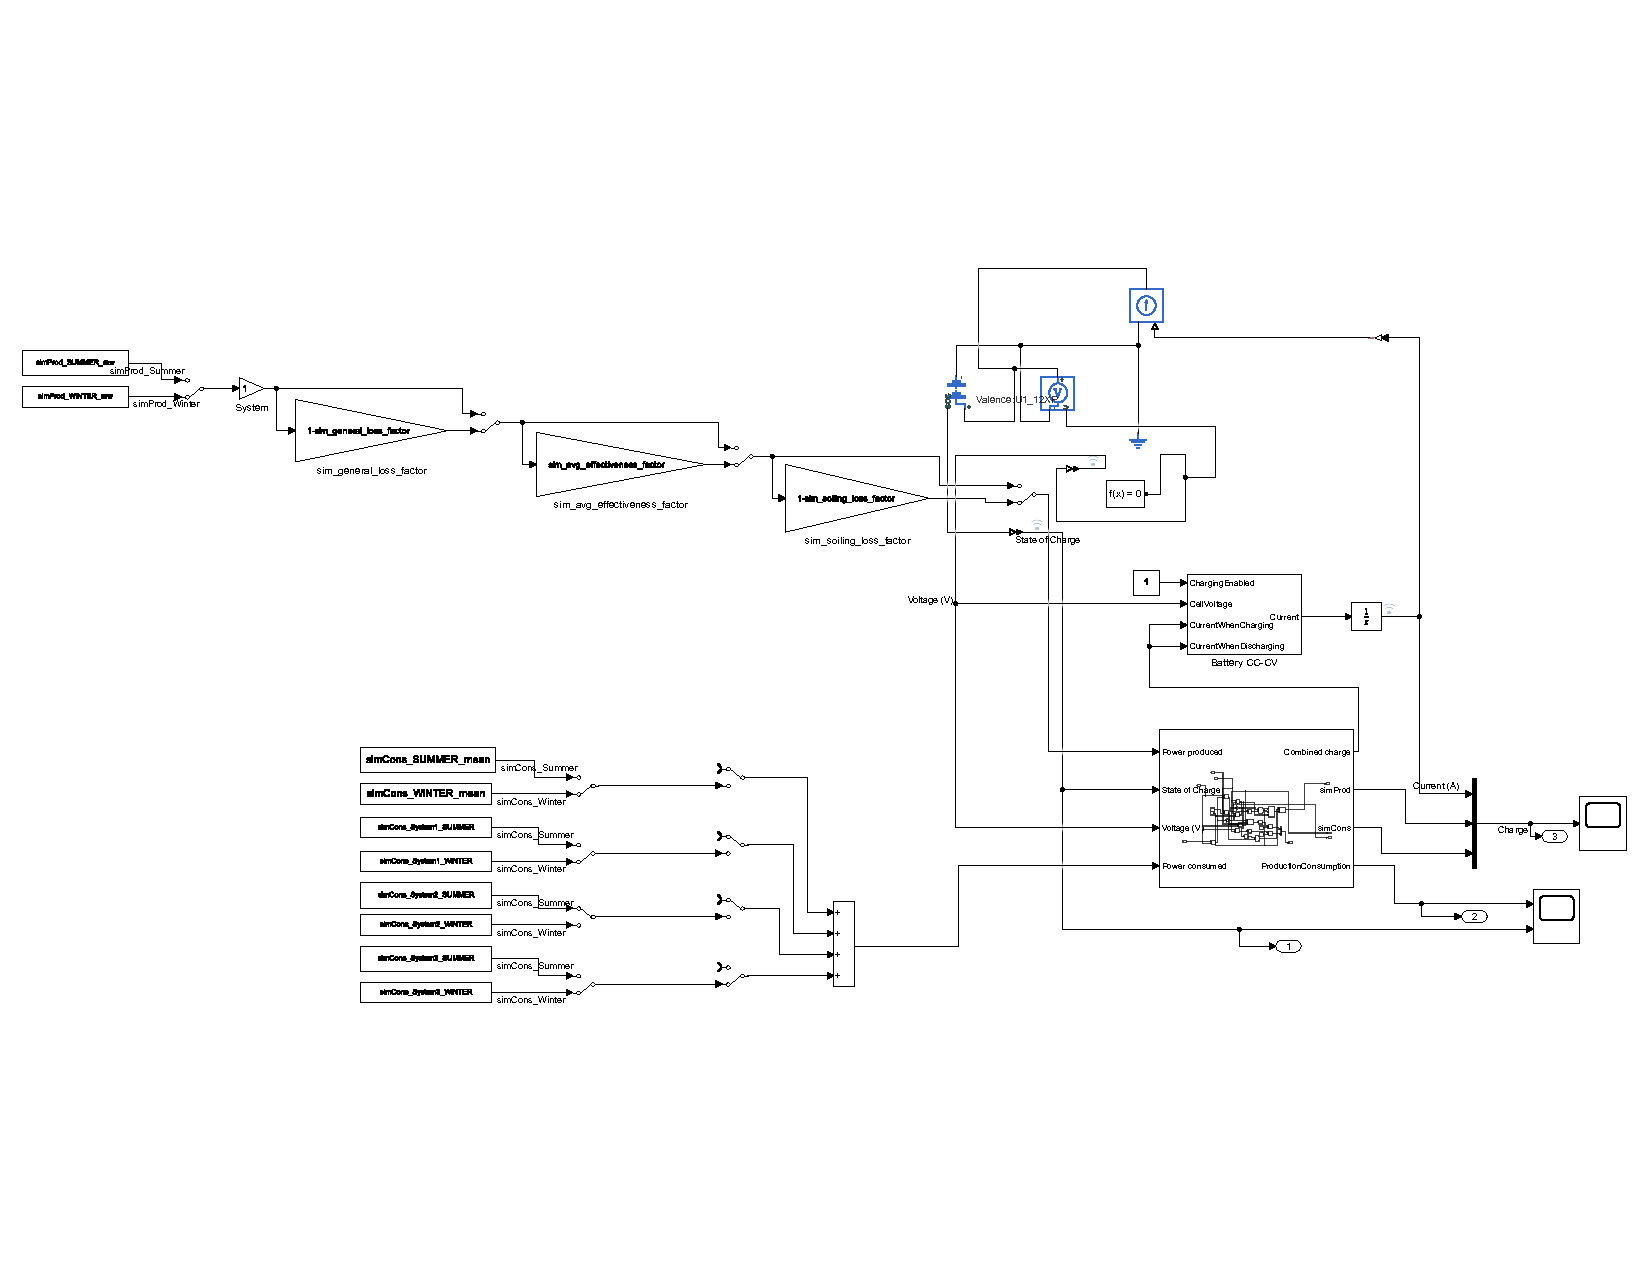
\includegraphics[width=\linewidth]{photos/Simulink.pdf}
\end{figure}


%-----------------------------------------------------------------
% \backmatter

\label{Bibliography}
% \lhead{\emph{Bibliography}}  % Change the left side page header to "Bibliography"



\printbibliography  % Print the bibliography
\uisbackcover
\end{document}